\documentclass[compress, ucs, xelatex, 11pt, xcolor=svgnames, aspectratio=169,
	hyperref={
		bookmarks=true,
		unicode=true,
		colorlinks=true,
		pdftitle={Linux, command line and MetaCentrum},
		plainpages=false,
		pdfauthor={Vojtech Zeisek},
		pdfsubject={Course about use of Linux command line, writing shell scripts and using MetaCentrum of CESNET},
		pdfcreator={XeLaTeX},
		pdfkeywords={Linux, GNU, BASH, shell, command line, MetaCentrum},
		linkcolor=DarkRed, % Navigation menu links on pages and in navigation menus
		anchorcolor=DarkBlue, % Not in use?
		citecolor=Indigo, % Not in use?
		filecolor=NavyBlue, % Not in use?
		menucolor=DarkMagenta, % Not in use?
		urlcolor=DarkBlue, % Links with \href and \url
		pdftex},
	url={hyphens, lowtilde} % Allow line breaks within URLs
	]{beamer}

% Theme settings
\usetheme[secheader]{Boadilla}
\usecolortheme{spruce}
\setbeamertemplate{headline} {
	\begin{beamercolorbox}{section in head/foot}
		\insertsectionnavigationhorizontal{\paperwidth}{\hskip0pt plus1fill}{\hskip0pt plus1fill}
	\end{beamercolorbox}
	\begin{beamercolorbox}[ht=2ex, dp=1.125ex]{subsection in head/foot}
		\insertsubsectionnavigationhorizontal{\paperwidth}{}{\hfill\hfill}
	\end{beamercolorbox}
	}
\useinnertheme{circles}

% Fonts Linux Libertine
\usepackage{libertine}

% Other packages
\usepackage{multicol}
\usepackage{array}

% In-line higlighting
\usepackage{soul}

% Add background for \texttt{}
\renewcommand{\texttt}[1]{\colorbox{Beige}{{\ttfamily #1}}}

% Change text color of highlighted text back to red
\renewcommand{\alert}[1]{\textcolor{red}{#1}}

% TeX logos
\usepackage{dtk-logos}

% Syntax higlight
\usepackage{minted}
\usemintedstyle{vim} % Styles are listed by pygmentize -L styles; languages are listed by pygmentize -L lexers
\newminted{bash}{linenos, fontsize=\footnotesize, bgcolor=Beige, fontfamily=tt, gobble=4, numbersep=-3pt}
% Change line number style
\renewcommand{\theFancyVerbLine}{
	\sffamily
	\textcolor{BlueViolet}{
		\tiny
		\oldstylenums{
			\arabic{FancyVerbLine}
			}
		}
	}

% Fixing space before and after block of code higlight
\BeforeBeginEnvironment{bashcode}{\vspace{-0.75em}}
\AfterEndEnvironment{bashcode}{\par\vspace{-0.5em}}

% Fixing space before and after multicols region
\BeforeBeginEnvironment{multicols}{\vspace{-0.5em}}
\AfterEndEnvironment{multicols}{\par\vspace{-0.5em}}

% Fixing space before and after itemize region
\BeforeBeginEnvironment{itemize}{\vspace{-0.25em}}
\AfterEndEnvironment{itemize}{\vspace{-0.25em}}

% Default language
\usepackage[main=american]{babel}

% Quotes
\usepackage[autostyle=true, english=american]{csquotes}

% Title page
\author{Vojtěch Zeisek}
\institute[\url{https://trapa.cz/}]{Department of Botany, Faculty of Science, Charles University, Prague\\Institute of Botany, Czech Academy of Sciences, Průhonice\\\url{https://trapa.cz/}, \href{mailto:zeisek@natur.cuni.cz}{zeisek@natur.cuni.cz}}
\title{Linux, command line \& MetaCentrum}
\subtitle{Use of Linux command line not only for CESNET's MetaCentrum}
\titlegraphic{\includegraphics[width=1cm]{tux.png}}
\date{January 17 to 20, 2022}

\begin{document}

\begin{frame}
	\titlepage
\end{frame}

\begin{frame}[allowframebreaks]{Outline}
	\tableofcontents
\end{frame}

\section{Introduction}

\begin{frame}{Introduction}{First steps in the world of Linux and open-source software}
	\tableofcontents[currentsection, sectionstyle=show/hide, hideothersubsections]
\end{frame}

\begin{frame}{The course information}
	\begin{itemize}
		\item The course page: \url{https://trapa.cz/en/course-linux-command-line-2022}
		\begin{itemize}
			\item Česky: \url{https://trapa.cz/cs/kurz-prikazove-radky-linuxu-2022}
		\end{itemize}
		\item Subject in SIS: \url{https://is.cuni.cz/studium/eng/predmety/index.php?do=predmet&kod=MB120C23}
		\begin{itemize}
			\item Česky: \url{https://is.cuni.cz/studium/predmety/index.php?do=predmet&kod=MB120C23}
			\item For students having subscribed the subject, requirements are on next slide
		\end{itemize}
		\item Working version of the presentation is available at \url{https://github.com/V-Z/course-linux-command-line-bash-scripting-metacentrum} --- feel free to contribute, request new parts or report bugs
	\end{itemize}
\end{frame}

\begin{frame}{Requirements to exam (\enquote{zápočet})}
	\begin{enumerate}
		\item Be present whole course.
		\item Be active --- ask and answer questions.
		\item Write short script solving any task the student is (going to be) solving. E.g. prepare script to process student's data on MetaCentrum. Or short script to do anything the student needs to do. This will be very individual. According to topics and interests of every student. Students can of course discuss with anyone, use Internet, manuals, etc. The aim is to learn how to solve real problem the student has/is going to have.
		\item Write at least one page (can be split into multiple articles) on Wikipedia about any topic discussed during the course. Again, this is very open, students can write about any topic they like. I~prefer native language of the student (typically to make larger non-English Wikipedia).
	\end{enumerate}
\end{frame}

\begin{frame}{Materials to help you\ldots}
	\label{materials}
	\begin{itemize}
		\item Download the presentation from \url{https://soubory.trapa.cz/linuxcourse/linux_bash_metacentrum_course.pdf}
		\item Download the scripts and toy data from \url{https://soubory.trapa.cz/linuxcourse/scripts_data.zip}
		\begin{itemize}
			\item \alert{Note:} Open the scripts in some \alert{good} text editor (slide~\ref{editors}) --- showing syntax highlight, line numbers, etc. (\alert{NO} Windows notepad); the files are in UTF-8 encoding and with UNIX end of lines (so that too silly programs like Windows notepad won't be able to open them correctly)
			\item \alert{Never ever} open any script file in software like MS~Word --- they destroy quotation marks and other things by \enquote{typographical enhancements} making the script unusable
		\end{itemize}
	\end{itemize}
\end{frame}

\subsection{Learning machine}

\begin{frame}{Virtual machine for learning}
	\label{VBox}
	\begin{multicols}{2}
		\begin{itemize}
			\item If you do not have Linux installed, download and install VirtualBox from \url{https://www.virtualbox.org/}
			\item Download openSUSE Leap 15.3 Linux distribution for this course from \url{https://botany.natur.cuni.cz/zeisek/openSUSE_Leap_courses.ova} ($\sim$4.6~GB)
			\item Launch VirtualBox and go to menu \textbf{File | Import appliance\ldots} to import it. When done, launch it (\textbf{Start})
			\item See also \url{https://trapa.cz/en/node/128}
		\end{itemize}
		\includegraphics[height=6.5cm]{virtualbox.png}
	\end{multicols}
\end{frame}

\begin{frame}{Enjoy learning virtual machine for the course}
	\begin{center}
		\includegraphics[height=6.5cm]{opensuse_leap_course.png}
	\end{center}
\end{frame}

\begin{frame}{VirtualBox shared folder I}{VirtualBox can be configured to share folder with host operating system}
	\begin{center}
		\includegraphics[height=6cm]{virtualbox_shared_folder_1.png}
	\end{center}
\end{frame}

\begin{frame}[fragile]{VirtualBox shared folder II}{Go to menu \enquote{Devices | Shared Folders} and set pair of folders}
	\begin{bashcode}
    sudo mount -t vboxsf -o uid=$UID,gid=$(id -g) shared /mnt
	\end{bashcode}
	\vfil
	\begin{center}
		\includegraphics[height=5.5cm]{virtualbox_shared_folder_2.png}
	\end{center}
	\vfill
\end{frame}

\subsection{What it is a~\enquote{UNIX}}

\begin{frame}[allowframebreaks]{What it is UNIX, Linux and GNU}
	\begin{itemize}
		\item \href{https://en.wikipedia.org/wiki/Unix}{UNIX}
		\begin{itemize}
			\item Originally developed in Bell labs of AT\&T in 1969, written in C, since then  huge radiation, hybridization, HGT,~\ldots
			\item Trademark --- only systems passing certain conditions (paid certification) can be called \enquote{UNIX} --- Solaris, HP-UX, AIX, etc. (commercial systems for big servers)
			\item Main principles: simple, multitasking, hierarchical, network, for more users (takes cares about permissions etc.), configuration written in plain text files, important relationships among applications (generally one application = one task --- they are chained), work primarily with text, has kernel and API (interface to communicate with the rest of the system)
			\item \href{https://en.wikipedia.org/wiki/Unix-like}{UNIX-like} (UN*X, *nix)
			\begin{itemize}
				\item Systems compatible with UNIX (Linux, BSD and its variants, macOS,~\ldots)
				\item Mainly open-source (UNIX is commonly commercial --- source code is not publicaly available, but its specification is)
				\item Nowadays prevailing over \enquote{old} UNIX systems, used in many devices from tiny embedded toys to huge data centers
				\item Try to provide same quality as paid systems, but (mostly) for free
			\end{itemize}
			\item Many courts about copyrights, parts of code, patents (USA allow software patents, EU not) --- GNU, Linux, BSD, etc. try to ensure to have only code not covered by any patents to avoid possible courts
		\end{itemize}
		\item \href{https://www.gnu.org/}{GNU}
		\begin{itemize}
			\item \enquote{GNU's Not Unix!} --- but it is compatible, respects its principles
			\item System written from scratch, following ideas of UNIX
			\item Since 1984 Richard Stallman (founder of \href{https://www.fsf.org/}{Free Software Foundation}) tried to make new kernel (Hurd --- not finished yet\ldots)
			\item Generally set of basic system tools --- working with many kernels (Linux, BSD*, macOS,~\ldots), also present in many commercial paid UNIX systems
			\item Source code is free and open --- anyone can study it (Security!), report bugs, contribute, modify, share it,~\ldots
			\item GNU General Public License (GPL) --- free spirit of open-source --- license, idea, how to share software
			\item Inspired open public software development --- crucial for our usage of Linux \& al.
		\end{itemize}
		\item \href{https://en.wikipedia.org/wiki/Linux}{Linux}
		\begin{itemize}
			\item First version of kernel (core of the system) written by Linus Torvalds in Helsinki in 1991
			\item Kernel was in principle inspired by various UNIX systems and using GNU tools for standard work
			\item Quickly became popular --- anyone can take it and use for any needs, adopt (modify it), etc.
			\item Used in small embedded (commonly network) devices, mobile devices (book readers, Android,~\ldots), personal computers, servers (from home level to biggest data centers),~\ldots
			\item Nowadays powering most of the Internet
			\item Anyone can contribute --- not only code, also documentation, design, translations,~\ldots
			\item Most of people working with UNIX are using Linux (or macOS)
		\end{itemize}
		\item GNU and Linux are two important (but not sole) pieces of building set forming modern operating system
		\item \enquote{Linux} nowadays usually mean Linux kernel + GNU basic tools  (thus correctly \enquote{GNU/Linux}) + thousands of various another applications (= \enquote{Linux distribution})
	\end{itemize}
\end{frame}

\begin{frame}{Extremely simplified UNIX phylogeny}
	\begin{center}
		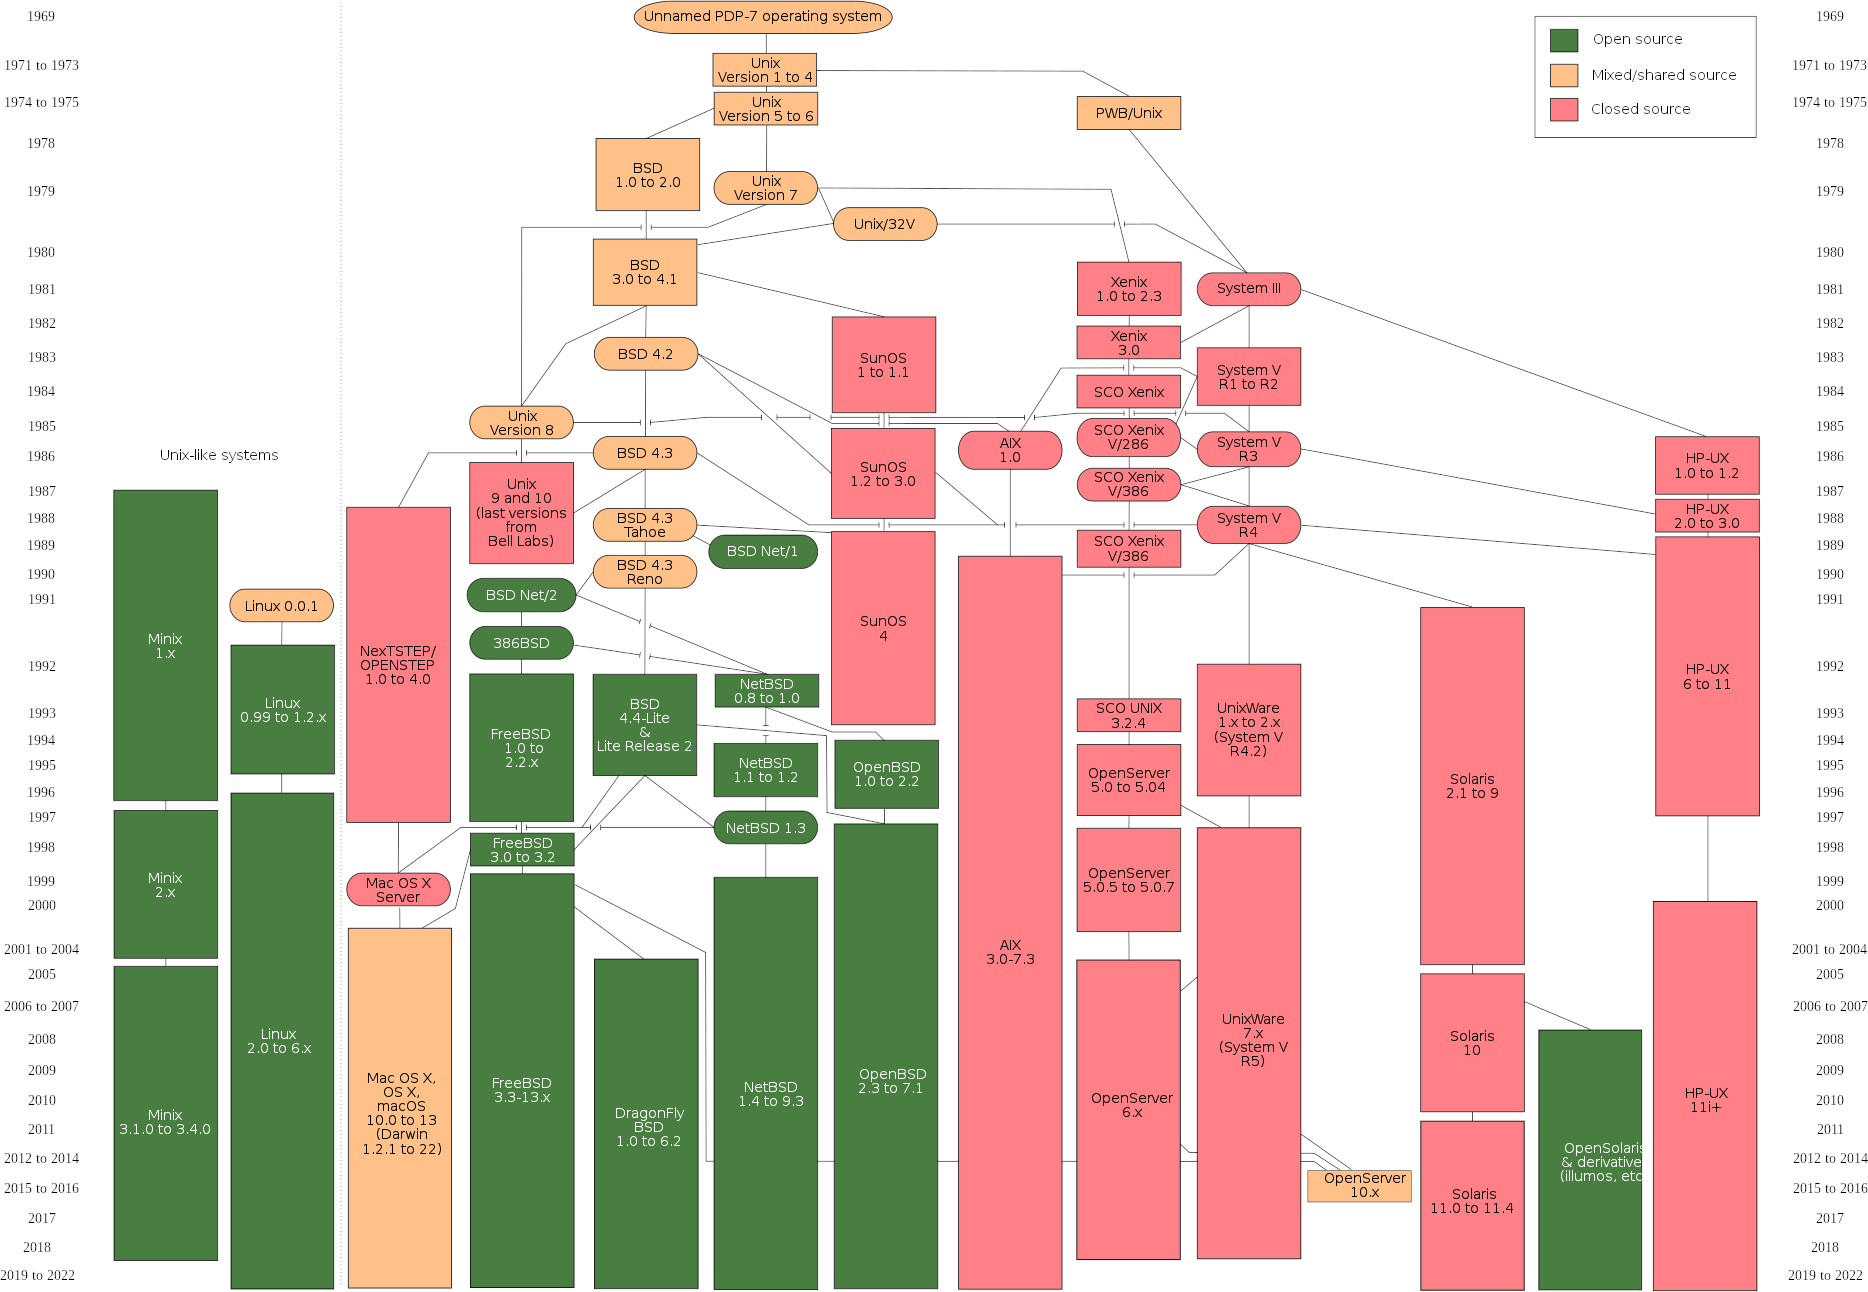
\includegraphics[height=6.5cm]{unix_history-simple.png}
	\end{center}
\end{frame}

\begin{frame}{Most common UNIX-based systems (except Linux)}
	\begin{itemize}
		\item \href{https://en.wikipedia.org/wiki/macOS}{macOS} (previously Mac OS~X) --- system kernel is based on older BSD and uses plenty of GNU tools (although mostly older outdated versions)
		\item \href{https://en.wikipedia.org/wiki/Berkeley_Software_Distribution}{BSD} --- one of the oldest operating systems, still developed in \href{https://distrowatch.com/search.php?ostype=BSD}{many independent variants}
		\begin{itemize}
			\item Still very popular especially on servers, for special purposes, etc.
			\item License allows closing of the code --- used by Apple macOS kernel, PlayStation firmware,~\ldots
			\item Installation and management is for beginners usually harder than Linux, everything must be done manually, not so common as Linux anymore
			\item E.g. \href{https://www.freebsd.org/}{FreeBSD}, \href{https://www.dragonflybsd.org/}{DragonFly BSD}, \href{https://www.openbsd.org/}{OpenBSD}, \href{https://www.truenas.com/}{TrueNAS} (for storage servers),~\ldots
		\end{itemize}
		\item \href{https://en.wikipedia.org/wiki/Solaris_(operating_system)}{Solaris} --- commercial, not very common
		\begin{itemize}
			\item Mainly special servers, paid
			\item \href{https://distrowatch.com/search.php?ostype=Solaris}{Several community-based variants} freely available
		\end{itemize}
		\item Command line usage is nearly same across UN*X systems --- all follow same standards, use more or less same set of tools
	\end{itemize}
\end{frame}

\subsection{Licenses and money}

\begin{frame}{Cathedral vs. market place}{What is principal difference between free open-source and commercial software}
	\begin{itemize}
		\item Commercial software is like a~cathedral
		\begin{itemize}
			\item Pay big money and get it in the state which the architect like
			\item User can not modify it (or it is terribly expensive)
			\item Might be you don't need everything --- but still paying whole set
		\end{itemize}
		\item Free open-source software (FOSS) is like a~market place
		\begin{itemize}
			\item Find there many producers of same tools --- pick up those you like --- freedom of choice
			\item Take exactly the tools you need --- any combination is possible
			\item Much cheaper to shop there
		\end{itemize}
		\item Both have pros and cons --- depends what you wish\ldots
		\item Consider e.g. difference between usage of full-featured and expensive Geneious (theoretically everything you need to process genetic data) vs. searching for hundreds of tools and pipelines on the Internet (GitHub, R packages, fora,~\ldots)
		\item According to \href{https://en.wikipedia.org/wiki/The_Cathedral_and_the_Bazaar}{book by Eric S.~Raymond}
	\end{itemize}
\end{frame}

\begin{frame}[allowframebreaks]{Free and open-source software --- (F)OSS}
	\begin{itemize}
		\item \textbf{Free like freedom of speech, \alert{not} like free beer!}
		\item Open-source --- source code can be seen by the holder of the license (not necessary by everyone)
		\item Not every OSS (generally less strict conditions) has to be \textbf{F}OSS (you can do with it (almost) whatever you like) --- source code might be available under some circumstance (only to look), but modification and/or reuse of the code prohibited (and then it is not \textbf{free})
		\item \href{https://www.gnu.org/licenses/gpl-3.0.html}{GNU GPL} (\enquote{\href{https://www.gnu.org/copyleft/}{copyleft}}) --- probably most common OSS license, strict, viral --- derived code has to keep the license --- surprisingly not fully \enquote{free} as it doesn't allow changes of license
		\item \href{https://www.gnu.org/licenses/lgpl-3.0.en.html}{LGPL} --- Lesser GPL --- more permissive
		\item \href{https://en.wikipedia.org/wiki/BSD_licenses}{BSD license} --- permissive --- allow derived code to became closed-source (commonly used by e.g. Apple macOS, Safari browser, small electronics,~\ldots)
		\item \href{https://www.apache.org/licenses/}{Apache} or \href{https://www.mozilla.org/MPL/}{Mozilla} licenses etc. --- specific use in particular software
		\item Creative Commons (CC) --- software licenses are not suitable for multimedia, text, etc. --- CC has many options (including denial of reuse of the product), see \url{https://creativecommons.org/}
		\item And \href{https://en.wikipedia.org/wiki/Comparison_of_free_and_open-source_software_licenses}{many} \href{https://opensource.org/licenses}{more} licenses\ldots
	\end{itemize}
	\begin{block}{Spirit of FOSS}
		\begin{itemize}
			\item Orientation might be tricky, but practical output for users is same --- \textbf{the software can be independently checked for bugs, backdoor, malware, can be improved and under some circumstances, new software can be derived, and usually, it is available for free}
			\item \alert{Aim is to \enquote{liberate} software to keep open sharing of ideas, mutual improve and security control}
			\begin{itemize}
				\item Although the point is clear, there are debates how to reach it\ldots
			\end{itemize}
		\end{itemize}
	\end{block}
	\begin{itemize}
		\item Practical output of using open-source licenses for the user
		\begin{itemize}
			\item Software can be used anywhere
			\item Software can be modified --- including various fixes of older code to work properly, or to different systems
			\item User can learn from the software (from the code), new software can be developed on top of it
			\item Easier to find and trace bugs
			\item Security --- no backdoors
			\item Bugs (problems) in the code can fixed by nearly anyone
			\item Often available for free
			\item Easier distribution of the software (can be copied into various repositories, like those of Linux distributions, \href{https://docs.conda.io/}{Conda} or \href{https://brew.sh/}{Homebrew})
		\end{itemize}
	\end{itemize}
\end{frame}

\begin{frame}{How to make money with free open-source software?}
	\begin{itemize}
		\item Traditional model --- user rents right (\enquote{buys a~license}) to use the software (and sometimes for support --- usually for extra money)
		\item Common mistake --- software is not \enquote{bought} --- only license is rented (\enquote{permission to use it} with many limitations)
		\item Software as service
		\begin{itemize}
			\item (F)OSS is available for free --- user can use it as it is or buy a~support --- help of any type
			\item No vendor lock-in --- user has the code, so he can modify the software himself, change provider of the services,~\ldots
			\item Cheap for user as well as company --- company specialized for one task, let's say server database, doesn't have to take care about the rest of the system --- someone else does; user pays only what he needs
			\item Our faculty is using \href{https://plone.org/}{Plone} system for web pages --- anyone can use it for free, someone (like we) asked a~company to help, and if we'd decided, we  could keep Plone and maintain it ourselves or find another company to help us with it
		\end{itemize}
	\end{itemize}
\end{frame}

\section{Linux}

\begin{frame}{Linux}{Generally about Linux}
	\tableofcontents[currentsection, sectionstyle=show/hide, hideothersubsections]
\end{frame}

\subsection{Generally about Linux}

\begin{frame}{What it is a~\enquote{Linux}}
	\begin{itemize}
		\item Operating system respecting principles of UNIX
		\item Components
		\begin{itemize}
			\item Linux \textbf{kernel} --- basic part of the system responsible for hardware and very basic low-level running of the system (\enquote{\textbf{Linux \textit{sensu stricto}}})
			\item GNU core utilities --- basic applications
			\item Graphical user environment (GUI) --- many choices
			\item Many other applications --- according to use --- whatever imaginable
		\end{itemize}
		\item Linux \textbf{distribution (\enquote{Linux \textit{sensu lato}})}
		\begin{itemize}
			\item Somehow assemble Linux kernel, basic tools and some applications
			\item Optionally add some patches and extra tools and gadgets
			\item Make your own design! (very important;)
			\item If lazy, remake existing distribution (using e.g. \href{http://openbuildservice.org/}{web service})
			\item Still surprised there are hundreds of them?
			\item It is like Lego --- pieces are more or less same across distributions, but result is very variable
			\item From \enquote{general} for daily use (pick up whatever you like) to very specialized --- special hardware devices, network services, rescue,~\ldots
		\end{itemize}
	\end{itemize}
\end{frame}

\begin{frame}{Linux kernel and other parts around it}
	\begin{center}
		\includegraphics[height=6cm]{linux_kernel_ubiquity.png}
	\end{center}
	\vfil
	\url{https://en.wikipedia.org/wiki/Linux_distribution}
	\vfill
\end{frame}

\begin{frame}{Extremely simplified adaptive radiation of Linux distributions}
	\begin{center}
		\includegraphics[height=5.5cm]{linux_fylogen_2.png}
	\end{center}
	\vfil
	\url{https://en.wikipedia.org/wiki/List_of_Linux_distributions} and \url{https://distrowatch.com/} ($\sim$850 distributions, $\sim$250 active)
	\vfill
\end{frame}

\subsection{Choose one}

\begin{frame}{Most common Linux distributions}
	\begin{itemize}
		\item \href{https://distrowatch.com/search.php?package=DEB}{Debian (DEB) based}
		\begin{itemize}
			\item \href{https://www.debian.org/}{Debian} --- one of oldest and most common, especially on servers
			\item \href{https://ubuntu.com/}{Ubuntu} (nowadays probably the most popular on PCs and notebooks) and derivatives --- \href{https://kubuntu.org/}{Kubuntu}, \href{https://xubuntu.org/}{Xubuntu}, \href{https://lubuntu.me/}{Lubuntu},~\ldots~(according to GUI used --- most of the system is same)
			\item \href{https://linuxmint.com/}{Mint} --- Based on Ubuntu as well as Debian, user-friendly, popular
			\item \href{https://www.kali.org/}{Kali}, \href{https://knopper.net/knoppix/index-en.html}{KNOPPIX}, \href{https://elementary.io/}{elementaryOS},~\ldots
		\end{itemize}
		\item \href{https://distrowatch.com/search.php?package=RPM}{Red Hat (RPM) based}
		\begin{itemize}
			\item \href{https://www.redhat.com/}{Red Hat} --- probably the most common commercial
			\item \href{https://getfedora.org/}{Fedora} --- \enquote{playground} for Red Hat --- very experimental
			\item \href{https://www.centos.org/}{Centos} --- Clone of Red Hat
			\item \href{https://www.opensuse.org/}{openSUSE} --- SUSE is second largest Linux company, openSUSE is community distribution (free) companion of SUSE Linux Enterprise
			\item \href{https://www.mageia.org/}{Mageia}, \href{https://www.pclinuxos.com/}{PCLinuxOS},~\ldots
		\end{itemize}
		\item \href{https://manjaro.org/}{Manjaro}, \href{https://getsol.us/}{Solus},~\ldots
		\item Android (practically Linux kernel, touch interface \& Java)
		\item For experienced users: Arch, Slackware, Gentoo,~\ldots
	\end{itemize}
\end{frame}

\begin{frame}{Graphical User Interfaces (GUI)}{More like \enquote{Mac-style}, \enquote{Windows-style} or something else? Feature rich or minimalistic?}
	\begin{itemize}
		\item Most of GUIs are available for most of common distributions --- one is picked as default and \enquote{only} color style is different
		\item \href{https://kde.org/}{KDE} --- one of the most common, feature extremely rich, basically \enquote{Windows-like} (can be changed), extremely versatile
		\item \href{https://www.gnome.org/}{GNOME} --- one of the most common, relatively simplistic interface, but still feature rich, \enquote{Mac-like}
		\item \href{https://xfce.org/}{XFCE} --- lightweight version of older GNOME --- for older computers or users not willing to be disturbed by graphical effects, basically \enquote{Mac-like} looking, but panels can be moved to \enquote{Windows style}
		\item \href{https://cinnamon-spices.linuxmint.com/}{Cinnamon} --- remake of GNOME to look more like Windows\ldots
		\item \href{https://code.launchpad.net/unity}{Unity} --- originally developed by Ubuntu (discontinued, now community based), \enquote{Mac-style}
		\item And much more\ldots
		\item Choose what you like --- doesn't matter much which one\ldots
	\end{itemize}
\end{frame}

\begin{frame}{Ubuntu with GNOME} % TODO Update print screen, add more
	\begin{center}
		\includegraphics[height=6.5cm]{ubuntu.png}
	\end{center}
\end{frame}

\begin{frame}{openSUSE with KDE --- Kubuntu is same, but blue\ldots} % TODO Update print screen, add more
	\begin{center}
		\includegraphics[height=6.5cm]{opensuse.png}
	\end{center}
\end{frame}

\begin{frame}{Fedora with GNOME --- GNOME is always almost same} % TODO Update print screen, add more
	\begin{center}
		\includegraphics[height=6.5cm]{fedora.png}
	\end{center}
\end{frame}

\begin{frame}{Linux Mint with Cinnamon} % TODO Update print screen, add more
	\begin{center}
		\includegraphics[height=6.5cm]{mint.png}
	\end{center}
\end{frame}

\begin{frame}{Debian with XFCE --- Xubuntu has more \enquote{modern} design} % TODO Update print screen, add more
	\begin{center}
		\includegraphics[height=6.5cm]{debian.png}
	\end{center}
\end{frame}

\begin{frame}{XFCE in Xubuntu, openSUSE, Fedora and Linux Mint} % TODO Update print screen
	\begin{center}
		\includegraphics[height=6.5cm]{xfce.png}
	\end{center}
\end{frame}

\begin{frame}{Dolphin (KDE file manager) --- default for openSUSE (inset) and after tuning in the same distribution\ldots} % TODO Update print screen
	\begin{center}
		\includegraphics[height=5.75cm]{dolphin.png}
	\end{center}
\end{frame}

% TODO More about GUI usage:
% * Editing DE settings
% * Managing global settings and applications
% * What is stored where

\begin{frame}[allowframebreaks]{How to try Linux?}
	\begin{itemize}
		\item Install it on some computer together with or instead of Windows
		\begin{itemize}
			\item If you can use whole disk, just boot from CD/USB and click \enquote{Next}\ldots
			\item If you don't have whole disk, you need at least one (commonly more) disk partition(s) --- if you don't know how to manage them, ask someone skilled\ldots
			\item Major updates of Windows 10 or Windows reainstalls use to destroy bootloader and it is not possible to start Linux anymore (although it can be usually easily fixed)
		\end{itemize}
		\item Live CD/USB
		\begin{itemize}
			\item The most easy --- burn ISO image of CD from web of almost any Linux distribution or use for example \href{https://unetbootin.github.io/}{UNetbootin} to prepare bootable flash
			\item You only have to know how to boot from CD/USB (usually press \texttt{ESC}, \texttt{DEL}, \texttt{F2}, \texttt{F10}, \texttt{F12},~\ldots{ }when starting computer --- varies according to manufacturer)
		\end{itemize}
		\item Virtualization (slide~\ref{VBox})
		\begin{itemize}
			\item Requires relatively powerful computer (preferable Intel i5 or i7 or AMD Ryzen and over 8~GB of RAM)
			\item Install virtual machine (probably the most easy is \href{https://www.virtualbox.org/}{VirtualBox}) --- allows install and run another operating system inside host as an ordinary application --- very easy and comfortable
		\end{itemize}
		\item Linux subsystem in MS Windows Store (Windows 10 and 11)
		\begin{itemize}
			\item To install follow \url{https://docs.microsoft.com/windows/wsl/about}
			\item Version 1 only for command-line applications (it has some problems with paths, text files,~\ldots), version 2 should allow GUI (experimental)
			\item Version 2 works well for most of tasks
		\end{itemize}
		\item Cygwin
		\begin{itemize}
			\item Download and install from \url{https://www.cygwin.com/}
			\item It is not native Linux, it is collection of GNU and open-source utilities compiled to work on Windows
			\item Follows POSIX standards (i.e. it works like normal UNIX command line, with all features)
			\item Every application must be specially compiled to be able to work under Cygwin (it is sometimes complicated)
			\item Collection is large, include also GUI and DE, but not everything is easy working
			\item Installation of custom software might be very hard\ldots
		\end{itemize}
	\end{itemize}
\end{frame}

\subsection{Differences}

\begin{frame}{The Linux diversity\ldots}
	\begin{itemize}
		\item Try several distributions and just choose one you like\ldots
		\item If selecting among the most common, it doesn't matter much which one you pick up
		\item Which design do you like?
		\item Which distribution is your friend or colleague using? To have someone to ask for help\ldots
		\item You can change GUI (or its design) without change of distribution, it use to be highly configurable
		\item Applications are still same --- no difference in Firefox across distributions --- keep your settings when changing distribution
		\item Everyone using Android is using Linux --- install some terminal emulator there :-)
		\item Special use --- \href{https://www.truenas.com/}{TrueNAS} for home as well as business file servers, \href{https://partedmagic.com/}{Parted Magic} and/or \href{https://www.system-rescue.org/}{SystemRescue} to repair broken system (disk failure) and save data,~\ldots
	\end{itemize}
\end{frame}

\begin{frame}{Differences among (common) Linux distributions}
	\begin{itemize}
		\item Design and colors ;-)
		\item Default GUI (others can be installed)
		\item Applications available right after installation
		\item Default settings (not much)
		\item Package management --- especially in command line
		\item Development model --- conservative or experimental, fast or slow
		\item Management of system services (how to start/stop certain services like database or web server) --- not important for daily usage for most of users
		\item Sometimes in location of some system files (can be customized) --- also not important in daily usage of most of users
		\item Kernel is almost same, applications are same and used in same way\ldots
		\item Command line is almost same across Linux, and almost same as in other UNIX systems (macOS,~\ldots)
	\end{itemize}
\end{frame}

\section{UN*X}

\begin{frame}{UN*X}{Theory and principles of UNIX-based operating systems}
	\tableofcontents[currentsection, sectionstyle=show/hide, hideothersubsections]
\end{frame}

\subsection{Disks and file systems}

\begin{frame}{Short overview of hard disk layout}
	\begin{itemize}
		\item Physical disk (piece of hardware) has at least 1~partition --- division seen in Windows as \enquote{disks} (\texttt{C}, \texttt{D},~\ldots) and mounted directory in UNIX
		\item MBR --- older description of disk division, up to 4~primary partitions (OS typically requires at leas one to run), one can be extended and contain more partitions, disks up to 2~TB
		\item GPT --- newer, no relevant limits, requires UEFI (replacement of BIOS --- responsible of start of nowadays computers)
		\item If unsure what to do, high probability to break it\ldots
		\item Blank new partition has to be formatted to desired file system according to use and target operating system
		\item Linux distributions have easy graphical tools to manage disk partitions (e.g. \href{https://gparted.org/}{GParted})
		\item \alert{Always have backup before such management!}
	\end{itemize}
\end{frame}

\begin{frame}{Comparison of file systems (limits and compatibility)}
	\label{fs}
	\begin{center}
		\begin{footnotesize}
			\begin{tabular}{ccccccc}
				\textbf{FS name} & \begin{tabular}[x]{@{}c@{}}\textbf{Name}\\\textbf{length}\end{tabular} & \textbf{Signs in name} & \textbf{Path length} & \textbf{File size} & \begin{tabular}[x]{@{}c@{}}\textbf{Partition}\\\textbf{size}\end{tabular} & \textbf{Supported systems}\\
				FAT32 & 255 & Unicode & No limit defined & 4 GiB & 2 TiB & Any\\
				exFAT & 255 & ? & No limit defined & 16 EiB & 64 ZiB & Any\\
				NTFS & 255 & Variable & Variable & 16 TiB & 16 EiB & Windows (UN*X)\\
				HFS+ & 255 & Unicode & Unlimited & 8 EiB & 8 EiB & macOS\\
				ext4 & 255 & Any, not / & No limit defined & 16 TiB & 1 EiB & Linux (UN*X)\\
				XFS & 255 & Any & No limit defined & 9 EiB & 9 EiB & Linux (UN*X)\\
				Btrfs & 255 & Any & No limit defined & 16 EiB & 16 EiB & Linux (only?)\\
				ZFS & 255 & Unicode & No limit defined & 16 EiB & 256 ZiB & UN*X
			\end{tabular}
		\end{footnotesize}
	\end{center}
	\begin{itemize}
		\item FAT32 (including extensions) is old-fashioned and not reliable FS, but still common in various flash disks and memory cards
		\item NTFS (basic Windows FS) and FAT do not support UNIX permissions, so they can't be used as system partition in Linux; see also \href{https://en.wikipedia.org/wiki/Comparison_of_file_systems}{full comparison}
		\item Btrfs, ext4, XFS and ZFS are not accessible from Windows at all (Linux mainly uses ext4)
		\item Btrfs, XFS and ZFS are the most advanced FS in common use
	\end{itemize}
\end{frame}

\begin{frame}[allowframebreaks]{Creation and control of FS}
	\begin{center}
		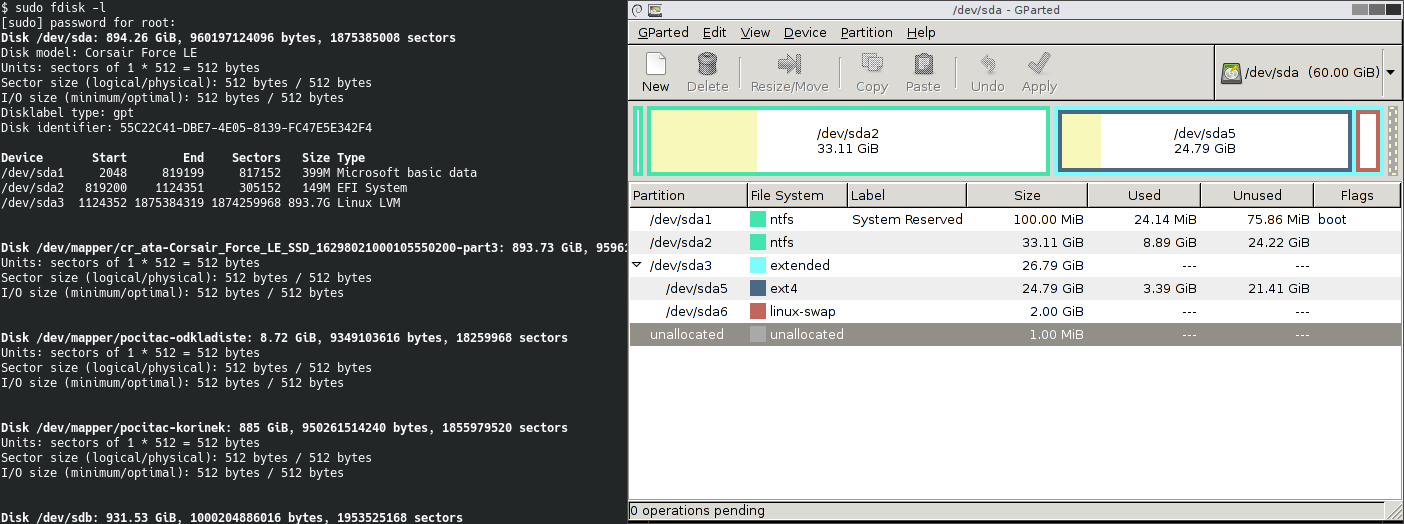
\includegraphics[width=\textwidth]{disks.png}
	\end{center}
	\begin{itemize}
		\item Work in command line or use graphical tool like \href{https://gparted.org/}{GParted}\ldots
		\item All commands require root privileges (slide~\ref{root})
		\item \texttt{fdisk -l} lists disks and partitions
		\item To manage disk partitioning use \texttt{fdisk /dev/sdX} or \texttt{gdisk /dev/sdX}
		\item When hard drive is partitioned, partitions must be formatted in next step
		\item Commands \texttt{mkfs.*} create various FS, common syntax is \texttt{mkfs.XXX -parameters /dev/sdXY}, where sdXY is particular disk partition
		\item Parameters can set label and various settings of behavior of the disk partition, check \texttt{man mkfs.XXX}
		\item To check FS for errors use \texttt{fsck.XXX /dev/sdXY} (according to respective FS)
		\begin{itemize}
			\item The filesystem must be unmounted when checking it
			\item XFS uses \texttt{xfs\_repair /dev/sdXY}
			\item Btrfs uses \texttt{btrfs check /dev/sdXY}, if it is unmountable, \texttt{btrfs-zero-log /dev/XY} use to help, last instance is \texttt{btrfs check -{-}repair /dev/sdXY} (dangerous operation)
			\item If Btrfs is mountable, but there are various FS errors and/or performance issues, \texttt{btrfs scrub start -Bdf /mount/point}, \texttt{btrfs filesystem defragment -r -v /mount/point} and \texttt{btrfs balance start -v /mount/point} --- manual running can take long time and strongly slow down the computer
		\end{itemize}
		\item \texttt{tune2fs -parameters /dev/sdXY} can set various parameters to influence behavior of disk (labels and more) partition
		\item \texttt{hdparm -parameters /dev/sdX} can set advanced hardware parameters of hard drive
		\item The most convenient is using graphical tools available in all distributions\ldots
		\begin{itemize}
			\item In \href{https://en.opensuse.org/Portal:YaST}{openSUSE there is YaST} administrative module --- from command line launch \texttt{yast -{-}qt partitioner} for graphical or \texttt{yast disk} for text-based version
			\item All distributions have graphical tools like \href{https://gparted.org/}{GParted} where it is possible to comfortable manage disks
		\end{itemize}
		\item \texttt{df -h} shows available/occupied space on disks/partitions, but because of special features of Btrfs it doesn't show every time correct values for this FS --- it is better to use \texttt{btrfs filesystem df /mount/point} (\texttt{/mount/point} use to be the most commonly \texttt{/})
		\item On UNIX FS, defragmentation and another maintenance tasks use to be done in background when computer is idling --- unless there is at least $\sim$20\% of free space on the device, this is not any problem and there are no performance issues
		\item \alert{Users must be sure what they are doing, otherwise system can be damaged}
	\end{itemize}
\end{frame}

\begin{frame}[fragile]{Another manipulations and information}
	\begin{itemize}
		\item \texttt{dd} is powerful, but potentially dangerous tool used to backup or write disks or partitions (commonly to create bootable USB media)
		\item If writing disk image to the disk (\texttt{sdX}), disk's partition table is discarded and the disk is covered by whatever is in the ISO image
	\end{itemize}
	\begin{bashcode}
    dmesg # Recent entries in main system log - filter with grep, tail, ...
    dmesg | grep sd | tail # Get information about recently plugged media
    # dd produces physical copy of whole device - including empty space
    dd if=/dev/sdX of=image.iso # Backups disk sdXY to imago.iso
    dd if=image.iso of=/dev/sdX # Used to write e.g. image of Linux live
                                # media to USB flash disk (Check sdX!)
    lnav # Comfortably browse recent logs, quit by "q"
	\end{bashcode}
	\begin{itemize}
		\item If there are encrypted partitions, they are in \texttt{/dev/mapper/\ldots}
		\item If LVM (slide~\ref{LVMRAID}) is used, see \texttt{lvscan} and \texttt{pvscan} to find correct location in \texttt{/dev/}
		\item Disks are also accessible through \texttt{/dev/disk/by-<TAB><TAB>}
	\end{itemize}
\end{frame}

\begin{frame}[fragile]{Mounting and unmounting disks and removable media}
	\begin{itemize}
		\item Mounting and unmounting of devices require root privileges
		\item In modern desktop Linux distributions, mounting is done automatically and media are visible mostly in \texttt{/media} or \texttt{/run/media}
		\item In Linux, physical disks are named from \texttt{sda} to \texttt{sdz}, each disk has partitions (at least one) numbered from \texttt{1}, (\texttt{sda1}, \texttt{sda2}, \texttt{sdb1},~\ldots), all are in \texttt{/dev} (\texttt{/dev/sdc3})
	\end{itemize}
	\begin{bashcode}
    eject # Open CD/DVD drive
    mount # Which FS (disk partitions) are mounted
    findmnt # See mounted devices in tree-like structure
    mkdir /mnt/point # Empty directory must exist prior mounting into it
    # mount usually recognize FS of mounted device, if not, add '-t FS_type'
    mount /dev/sdXY /mount/directory # Mount disk sdXY to /mount/directory
    mount -t iso9660 -o loop file.iso /mnt/iso # Mount CD/DVD ISO file
    umount /dev/sdXY # Unmount disk sdXY, alternatively use below command
    umount /mount/directory # Unmount disk from /mount/directory
	\end{bashcode}
\end{frame}

\begin{frame}{Put together more disks}{Extend space and get higher data security}
	\label{LVMRAID}
	\begin{itemize}
		\item \href{https://en.wikipedia.org/wiki/RAID}{RAID} --- Redundant Array of Inexpensive/Independent Disks
		\item RAID~0~--- stripping, no redundancy, no security, speed up (two or more disks joined into one, files divided among disks)
		\item RAID~1~--- mirroring --- even number of disks of same size --- resulting capacity is half, very fast, secure
		\item RAID~5~--- at least three disks, one is used for parity control (in RAID~6 two disks are used for parity control), little bit slower, popular in cheaper storage servers (NAS)
		\item Combinations (RAID~10,~\ldots)
		\item \href{https://en.wikipedia.org/wiki/Logical_volume_management}{LVM} --- Logical Volume Management --- built over several partitions/disks --- seen by OS as one continuous space, can be dynamically managed
		\item Functionality of RAID and LVM (and more) is more or less covered by Btrfs and ZFS
	\end{itemize}
\end{frame}

\subsection{Types of users}

\begin{frame}{Root vs. \enquote{normal} user}
	\label{root}
	\begin{itemize}
		\item Root is administrator --- more than God (of the server) --- can do anything
		\item Other users have limited permissions
		\begin{itemize}
			\item System users providing particular service (web server, database, networking service) are as restricted as possible to do the task --- security
			\item \enquote{Human} users don't have access to system files (at least not for modification), homes of users are separated
		\end{itemize}
	\end{itemize}
	\begin{center}
		\includegraphics[height=3.5cm]{sandwich.png}
	\end{center}
	\begin{flushright}
		\url{https://xkcd.com/149/}
	\end{flushright}
\end{frame}

\begin{frame}[fragile]{Becoming root}
	\begin{itemize}
		\item Root privileges are required for any administrative task (install of software package, change of system settings,~\ldots)
		\item Word \enquote{root} is used as name for system administrator user, and also for top of filesystem directory hierarchy (\texttt{/})
	\end{itemize}
	\begin{bashcode}
    # Gain root privileges
    su # Requires root password (stay in current directory)
    su - # Requires root password (go to /root)
    su -c "some command" # Launch one command with root permissions
    su USER # Became USER (USER's password is required)
    sudo -i # For trusted users, became root (asks for user's password)
            # User has to be listed in /etc/sudoers
    sudo somecommand # Launch somecommand with root's privileges - can be
                     # restricted for particular commands; /etc/sudoers can
                     # contain special settings for particular users/groups
    cat /etc/passwd # See all users (including system users)
	\end{bashcode}
\end{frame}

\subsection{Directory structure}

\begin{frame}[allowframebreaks]{Directory structure in Linux}
	\begin{itemize}
		\item It is similar also in another UN*X systems
		\item Directory structure in Linux is similar to macOS (but there it is bit hidden, users usually don't see everything), but very different from Windows logic
		\item Top directory \enquote{\texttt{/}} --- \enquote{root}
		\item Everything else (including disks and network shares) are mounted in subdirectories (\texttt{/\ldots})
		\item \texttt{/bin} --- very basic command line utilities
		\item \texttt{/boot} --- bootloader responsible for start of system
		\item \texttt{/dev} --- devices --- representations of disks, CD, RAM, USB devices,~\ldots
		\item \alert{\texttt{/etc}} --- system configuration in plain text files --- edit them to change system-wide settings (read documentation and comments there)
		\item \alert{\texttt{/home}} --- users' homes
		\item \texttt{/lib}, \texttt{/lib64} --- basic system libraries (32 and 64bits)
		\item \texttt{/lost+found} --- feature of FS, after crash and recovery of FS, restored files are there
		\item \alert{\texttt{/media}} --- attached disks (USB flash,~\ldots) usually appear there (might be in \texttt{/var/run/media} or  \texttt{/var/media}) --- subdirectories are automatically created when device is plugged and disappears when unplugged
		\item \texttt{/mnt} --- usually manually mounted file systems (but they can be mounted elsewhere according to needs)
		\item \texttt{/opt} --- optional, usually locally compiled software
		\item \texttt{/proc} --- dynamic information about system processes
		\item \texttt{/root} --- root's (admin's) home
		\item \texttt{/run} --- temporal ID files (locks) of running processes
		\item \texttt{/sbin} --- basic system utilities
		\item \texttt{/selinux} --- SELinux is security framework
		\item \texttt{/srv} --- FTP and WWW server data (can be in \texttt{/var/srv})
		\item \texttt{/sys} --- basic system
		\item \texttt{/tmp} --- temporary files --- users have private dynamically created spaces there, used automatically by applications according to need
		\item \texttt{/usr} --- binaries (executable applications) and libraries of installed applications
		\item \alert{\texttt{/var}} --- data of most of applications and services, including e.g. database data, system logs,~\ldots
		\item \alert{\texttt{/windows}} --- if on dual boot, Windows disks are commonly mounted here
		\item In newest Linux distributions, most of \texttt{/bin}, \texttt{/etc}, \texttt{/lib}, \texttt{/lib64} and \texttt{/sbin} are mostly in \texttt{/usr} (original locations are just links)
		\item Can be altered, modified
		\item E.g. MetaCentrum has storage servers in various locations accessible from frontends and calculation nodes in \texttt{/storage}
		\item Usually, work only in your home, anywhere else modify files only if you are absolutely sure what you are doing
		\item Normal user doesn't have permission to modify files outside his directory (with exception of plugged removable media, etc.)
		\item Try \texttt{man hier} for details
	\end{itemize}
\end{frame}

\begin{frame}{Configuration in \texttt{/etc} (examples)}
	\begin{itemize}
		\item Configuration of system services (servers,~\ldots) and behavior
		\begin{itemize}
			\item Apache web server, database, FTP server, networking, basic system settings,~\ldots
		\end{itemize}
		\item \texttt{cron*} --- cron automatically repeatedly runs tasks
		\item \texttt{fstab} --- description of FS mounted during startup
		\item \texttt{group} --- list of users and groups
		\item \texttt{passwd} --- basic settings for users (home directory, default shell,~\ldots)
		\item \texttt{resolv.conf} ---  DNS settings (part of basic networking)
		\item \texttt{shadow} --- users passwords in encrypted form
		\item \texttt{skel} --- basic directories and configuration for new users
		\item Much more according to software installed\ldots
	\end{itemize}
\end{frame}

\begin{frame}[fragile]{Example of configuration in \texttt{/etc/ssh/sshd\_config}}
	\begin{bashcode}
    # This is the ssh client system-wide configuration file.  See
    # ssh_config(5) for more information.  This file provides defaults for
    # users, and the values can be changed in per-user configuration files
    # or on the command line.
    # ...
    Host *
    # If you do not trust your remote host (or its administrator), you
    # should not forward X11 connections to your local X11-display for
    # security reasons: Someone stealing the authentification data on the
    # remote side (the "spoofed" X-server by the remote sshd) can read your
    # keystrokes as you type, just like any other X11 client could do.
    # Set this to "no" here for global effect or in your own ~/.ssh/config
    # file if you want to have the remote X11 authentification data to
    # expire after twenty minutes after remote login.
    ForwardX11Trusted yes
    # ...
	\end{bashcode}
\end{frame}

\subsection{Files and directories}

\begin{frame}{Everything is (text) file}
	\begin{itemize}
		\item In UNIX specifications, everything is (text) file
		\begin{itemize}
			\item Technically, directory is \enquote{just} a~file listing its content
			\item Text files are easy to read, parse, manipulate
			\begin{itemize}
				\item Very easily editable (easy to change configuration)
				\item Easy to transfer to another system
				\item Easily comparable among users/versions/systems
			\end{itemize}
			\item UNIX command line tools are the most powerful when processing text files (of any sort, e.g. also genetic data)
		\end{itemize}
		\item When transferring to and from Windows, be aware of EOL and encoding (slide~\ref{eolenc})!
		\item FAT32 (commonly used for USB flash disks) has limits to maximal file size ($\sim4$~GB) and range of characters allowed in file name is limited (slide~\ref{fs}), it doesn't support UNIX permissions (breaks executability of scripts)
		\begin{itemize}
			\item Avoid large single files (or use archives to split large files)
			\item In file names keep only alphanumerical characters, dots and underscores (omit spaces and accented characters)
			\item Use archives to keep needed permissions (e.g. executability of scripts), see further
		\end{itemize}
		\end{itemize}
\end{frame}

\begin{frame}[fragile]{File names}
	\label{filenames}
	\begin{itemize}
		\item \alert{Space serves as separator of parameters}
		\item Linux allows \alert{any} character in file name, except \alert{slash} (\texttt{/}), so including anything on keyboard as well as line break (\alert{!}) --- be conservative\ldots
	\end{itemize}
	\begin{bashcode}
    mkdir My New Directory # Produces THREE directories (mkdir creates dirs;
                           # spaces separate parameters). Solutions:
    mkdir "My New Directory" # (you can use single quotes '...' as well) or
    mkdir My\ New\ Directory # "\" escapes following character
    rmdir My\ New\ Directory # Same problem and solution when removing it
    touch \* # Creates new empty file named just * (yes, asterisk)
    rm * # What would be removed? :-) Solution: rm \* or rm '*'
	\end{bashcode}
	\begin{itemize}
		\item Files and directories starting by \alert{dot} (\texttt{.} --- \texttt{.xxx\ldots}) are hidden by default (typically user settings and application data in user home)
	\end{itemize}
	\begin{bashcode}
    touch .hiddenfile # Let's make empty text file hidden by default
    ls # We will not see it (ls lists only "visible" files/directories)
    ls -a # We will see it ("-a" to see all - also hidden - files/dirs)
	\end{bashcode}
	\alert{Task:} Try everything on this slide, also with different file names and characters.
\end{frame}

\begin{frame}[fragile]{Types of files}
	\begin{bashcode}
    ls -la ~
    -rw-r--r-- 1 vojta users 1685 Feb 25  2019 .bashrc
    drwxr-xr-x 1 vojta users 1040 Jan  8 09:08 bin
    lrwxrwxrwx 1 vojta users   28 Jan 11 18:00 .lyxpipe.in -> /tmp/kile-...
    ...
	\end{bashcode}
	\vfill
	\begin{itemize}
		\item Regular file --- ordinary file, marked by dash (\texttt{-}) on beginning
		\item Directory --- in UNIX special type of file, marked by \texttt{d} on beginning
		\item Symbolic link (symlink, \enquote{soft link}) --- points to another place, marked by \texttt{l}, slide \ref{links}
		\item Hard link --- just another name for existing file, no special symbol, slide \ref{links}
		\item Block and character device --- in \texttt{/dev}, representations of devices (hard disks, terminals,~\ldots), marked by \texttt{b} or \texttt{c} respectively
		\item Named pipe --- pipe can be saved (by \texttt{mkfifo}), looks like a~file, more at slide \ref{pipe}
		\item Socket --- for communication among processes, also bidirectional, available on network
	\end{itemize}
\end{frame}

\begin{frame}[fragile]{Links}
	\label{links}
	\begin{itemize}
		\item \textbf{Symbolic (soft) links (symlinks)} --- like links on the web --- short-cut to another place
		\begin{itemize}
			\item When we delete link, nothing happens, when target, non-working link remains
		\end{itemize}
	\end{itemize}
	\vfill
	\begin{bashcode}
    ln -s target link_name # Link points to target (existing file/directory)
    ls -l bin/cinema5
    lrwxrwxrwx 1 vojta users 42 5. dub 2014 cinema5 -> # "l" marks link
      /home/vojta/bin/cinema5-0.2.1-beta/cinema5*      # "->" points to target
	\end{bashcode}
	\vfill
	\begin{itemize}
		\item \textbf{Hard links} --- only second name for file already presented on the disk (available only for files): \texttt{ln target link\_name}
		\begin{itemize}
			\item If any one of the two files is deleted, the second remains to be fully working
		\end{itemize}
	\end{itemize}
	\vfill
	\begin{bashcode}
    ln .bashrc .bashrcX
    ls -l .bash* # Numbers in first column show links pointing to it
                 # For directories - number of items, for files = 1
    -rw------- 1 vojta users 7298 21. jan 16.43 .bash_history # One link
    -rw-r--r-- 2 vojta users 2707 29. nov 16.21 .bashrc       # Same as below
    -rw-r--r-- 2 vojta users 2707 29. nov 16.21 .bashrcX      # Two links
	\end{bashcode}
\end{frame}

\subsection{Permissions}

\begin{frame}{Owner and group}
	\begin{itemize}
		\item Every file has an owner and group --- for finer setting of rights
		\item Group can have just one member --- the user
		\item System usually shows names of groups and users, but important are IDs (numbers): GID and UID
		\item Commands \texttt{chown} to change owner requires root privileges
		\item Commands \texttt{chgrp} to change group often requires root privileges --- user has to be member of particular group to be able to change ownership to it (if not, \texttt{root} must do it)
		\item Information about users and groups and their IDs are in \texttt{/etc/group} and \texttt{/etc/passwd}
		\item Ownership (and permissions, slide~\ref{permissions}) are important especially on servers with plenty of users (e.g. on MetaCentrum)
		\item It is not possible to add particular permissions for particular user on one file/directory --- there must be special group or ACL must be used (slide~\ref{acl})
	\end{itemize}
\end{frame}

\begin{frame}[fragile]{Change owner and/or group}
	\begin{bashcode}
    ls -l # Shows also owner and group (columns 3 and 4):
    drwxr-xr-x 1 vojta users    80  5. jan 16.12 linuxcourse
    drwxr-xr-x 1 vojta users  1648 31. jan 10.15 presentation
    -rw-r--r-- 1 vojta users  1944  5. jan 15.18 README
    drwxr-xr-x 1 vojta users   822 29. jan 10.12 scripts_data
    -rwxr-xr-x 1 vojta users  1126  5. jan 15.22 web_update.sh
    l # Common alias for 'ls -l' or 'ls -la' (according to distribution)
    ll # Common alias for 'ls -l' or 'ls -la' (according to distribution)
    id # Display UID and GIDs of current user
    # New owner or group can be defined as name or ID
    chown newowner:newgroup files # Change owner and group
    chown -R newowner files # Recursively (with subdirectories) change owner
    chgrp -R newgroup files # Recursively (with subdirectories) change group
    chown --help # Or 'man chown' for more options
    chgrp --help # Or 'man chgrp' for more options
	\end{bashcode}
	\begin{itemize}
		\item Equally important is to have correct permissions (especially on server) --- next slides
	\end{itemize}
\end{frame}

\begin{frame}{File and directory permissions}
	\label{permissions}
	\begin{itemize}
		\item Combination of permissions to read/write/execute for user(owner)/group members/others
	\end{itemize}
	\begin{center}
		\begin{tabular}{llll}
			\textbf{Permission} & \textbf{Number} & \textbf{Directory} & \textbf{File}\\
			r & 4 & Read directory content & Read file content\\
			w & 2 & Write into it (add/remove items) & Write into it, modify, delete it\\
			x & 1 & Enter it & Launch application (script)
		\end{tabular}
	\end{center}
	\begin{itemize}
		\item \texttt{rwxrw-r-{-}} --- 3$\times$3 characters for permissions for owner of the file/directory, group it is belonging to, and other users (\texttt{d} on beginning marks directories, \texttt{l} links, \texttt{+} ACL, slide \ref{acl})
		\item \texttt{764} --- same as above --- numbers for each role are summed --- first one is for owner, second for group and last for others
		\item Executable scripts and binaries \textbf{require} executable permission (\texttt{x}, e.g. \texttt{chmod +x} or \texttt{chmod u+x}) --- not supported on FAT drives (USB sticks, memory cards,~\ldots)
	\end{itemize}
\end{frame}

\begin{frame}[fragile]{Permissions examples}
	\begin{bashcode}
    ls -l # Shows permissions, links, owner, group, size, date, name
    # Only owner can read and write the file; 600:
    -rw-------   1 vojta users   38211 20. jan 09.23 .bash_history
    # Owner can write read and write the file, others read; 644:
    -rw-r--r--   1 vojta users    2707 29. nov 16.21 .bashrc
    # Owner can enter, read and write directory, others can read and enter it;
    # 755:
    drwxr-xr-x  41 vojta users    4096 27. pro 09.55 bin
    # Only owner can read, write and enter the directory, others nothing; 700:
    drwx------  58 vojta users    4096 17. pro 15.45 .config
    # Link, everyone can seemingly do everything; 777:
    lrwxrwxrwx   1 vojta users      37 20. jan 09.33 .lyxpipe.in ->
      /tmp/kde-vojta/kilemj7d3E/.lyxpipe.in # Check permissions of target!
    # Executable (application) - everyone can launch it, but only owner can
    # write into the file (change or delete); 755:
    -rwxr-xr-x   1 vojta users    2187 27. nov 13.10 strap.sh*
	\end{bashcode}
	\vfill
	\begin{itemize}
		\item Permission to \enquote{write} also means permission to \textbf{delete} it
	\end{itemize}
\end{frame}

\begin{frame}[fragile]{Check and modify permissions}
	\begin{bashcode}
    ls -l # Long list - file names and attributes
    ls -a # All, including hidden files (starting with dot)
    ls -F # Add on the end of name "/" for directories and "*" for executable
    ls -h # Human readable size units (use with -l or -s)
    ls --color ## Colored output
    ls -laFh --color # Combine any parameters you like
    chmod u/g/o/a+/-r/w/x FILE # For respective user/group/others/all adds
                               # /removes permission to read/write/execute
    chmod XYZ FILE # Instead of XYZ use number code of permission
    chmod -R # Recursive (including subdirectories)
    chmod +x script.sh # Make script.sh executable for everyone
    chmod o-r mydir # Remove read permission from others on mydir
    chmod 600 FILE1 FILE2 # Make both files R/W only by their owner
    chmod 000 FILE # No one can do anything - owner or root must add
                   # some permissions before any other action...
    chmod 777 * # All permissions for everyone on everything (no recursive)
    chmod --help # Or 'man chmod' for more options
	\end{bashcode}
\end{frame}

\begin{frame}[allowframebreaks]{Extending permissions --- ACL (Access control list)}
	\label{acl}
	\begin{itemize}
		\item By default, it is not possible to give specific permission to the user who is not owner, nor member of group owning the file
		\item In ext4 FS it has to be turned on manually (usually it is by default), it is part of Btrfs, XFS and ZFS --- it is not available on every computer/server
		\item Command \texttt{getfacl} lists those extra permissions, \texttt{setfacl} sets
		\item \alert{When in use, \enquote{basic} tools listing permissions (e.g. \texttt{ls -l}, ACL in use is marked by \texttt{+} after permissions --- next slide) sometimes do not show correct result and permissions may work unexpectedly}
		\item Important especially in network environment with many users
		\item If intensively used, \texttt{ls -l} sometimes doesn't show correct permissions (see next slide), it can be confusing and lead into various issues
		\item If not in use on server (like e.g. on CESNET data storage in Ostrava, \texttt{du4.cesnet.cz}), relatively high number of groups is required to be able to correctly setup sharing permissions
		\item MetaCentrum has storages and clusters connected via NFSv4 protocol (see also slide~\ref{netfs}) --- commands \texttt{getfacl} and \texttt{setfacl} do not work there, use \texttt{nfs4\_getfacl}, \texttt{nfs4\_setfacl} and \texttt{nfs4\_editfacl} instead (usage is very similar), see also \url{https://wiki.metacentrum.cz/wiki/Access_Control_Lists_on_NFSv4}
		\item Permissions (\enquote{classical} as well as ACL) require some time to practice and master it\ldots
	\end{itemize}
\end{frame}

\begin{frame}[fragile]{ACL examples}
	\begin{bashcode}
    getfacl FILE # get ACL for FILE:
    # file: dokumenty
    # owner: zeisek # Correct
    # group: zeisek # Correct
    user::rwx       # Correct
    user:nasik:r-x  # This is not seen from 'ls -l' output below!
    group::r-x      # This group has only one member, this is fine
    mask::r-x
    other::---      # Correct
    ls -l FILE # Compare this and previous output (This might be wrong!):
    drwxr-x---+  2 zeisek zeisek     6 17. zář 20.40 dokumenty/
    setfacl -m u/g:USER/GROUP:r/w/x FILE # Add for USER/GROUP r/w/x right
    # E.g. recursively add read permission to user 'arabidopsis_data' to
    # folder 'dokumenty/arabidopsis' (no extra group is required)
    setfacl -mR u:arabidopsis_data:r dokumenty/arabidopsis
    setfacl -R ... # Recursive (including subdirectories)
    setfacl -b FILE # Remove all ACL from FILE (combine with -R ...)
	\end{bashcode}
\end{frame}

\begin{frame}{Set default permissions for new files}
	\begin{itemize}
		\item \texttt{umask} sets implicit permissions for newly created files for user
		\item Syntax is similar to \texttt{chmod}, but reverse (e.g. \texttt{027} keeps all rights for owner, for group removes writing and nothing left for others)
		\begin{itemize}
			\item \texttt{umask} number \textbf{removes} certain permissions
		\end{itemize}
		\item \texttt{umask 027} (or other number) is typically set in file \texttt{$\sim$/.bashrc}
		\begin{itemize}
			\item \texttt{$\sim$} means user's home directory
			\item \texttt{.bashrc} is user's configuration for BASH (see slide~\ref{bashrc})
		\end{itemize}
		\item Typically used in network environment
		\item Set with care --- new permissions will have plenty of consequences --- different are typically needed for web pages, private files, shared files,~\ldots
		\item \texttt{umask} work recursively for all new files in user home directory --- it is not possible to set new implicit rules for particular directory
	\end{itemize}
\end{frame}

\begin{frame}[fragile]{Other permissions}
	\begin{itemize}
		\item \texttt{sticky bit} --- new directory/file in shared directory (where everyone can write) will be deletable only by owner (typically in \texttt{/tmp})
	\end{itemize}
	\vfill
	\begin{bashcode}
    chmod +t somedirectory
    ls -la /
    drwxrwxrwt 22 root root 800 21. jan 18.20 tmp # "t" marks it
	\end{bashcode}
	\vfill
	\begin{itemize}
		\item \texttt{setgid} --- application can have root permission even it was launched by normal user
	\end{itemize}
	\vfill
	\begin{bashcode}
    chmod u+s someapplication
    ls -al /bin/passwd
    -rwsr-xr-x 1 root shadow 51200 25. zář 08.38 /usr/bin/passwd # Note "s"
	\end{bashcode}
	\vfill
	\begin{itemize}
		\item \texttt{chattr} --- change of advanced attributes on Linux FS
		\item Mostly, there is no need to modify them
	\end{itemize}
	\vfill
	\begin{bashcode}
    chattr -RVf -+=aAcCdDeijsStTu files
    man chattr # See explanation of attributes
    lsattr # List extended attributes
	\end{bashcode}
\end{frame}

\subsection{Text}

\begin{frame}{Text and text --- differences among operating systems}
	\label{eolenc}
	\begin{itemize}
		\item Windows and UNIX have different internal symbol for end of line (\href{https://en.wikipedia.org/wiki/Newline}{new line}) --- EOL
		\begin{itemize}
			\item UNIX (Linux, macOS,~\ldots): LF (\texttt{\textbackslash n})
			\item Windows/DOS: CR+LF (\texttt{\textbackslash r\textbackslash n})
			\item Mac v. < 9: CR (\texttt{\textbackslash r}) (Mac up to 9~wasn't UN*X, since OS~X it is)
		\end{itemize}
		\item Good text editor (slide~\ref{editors}) can open correctly any EOL, but for example execution of script written in Windows will probably fail on Linux if it has wrong EOL
		\item Different systems use different encoding
		\begin{itemize}
			\item UNIX: mainly UTF-8 (Unicode, universal), UTF-16 for Asian languages
			\item Windows: win-cp-125X (variants according to region)
			\item Older UNIX: ISO-8859-X (variants according to region)
			\item Other much less common (historical) types\ldots
			\item Important mainly for accented characters
		\end{itemize}
		\item Text editors can usually open any encoding, but automatic detection commonly fails --- set it manually, see also slide~\ref{eolencoding}
	\end{itemize}
\end{frame}

\section{Command line}

\begin{frame}[allowframebreaks]{Command line}{Practical usage of command line tools}
	\tableofcontents[currentsection, sectionstyle=show/hide, hideothersubsections]
\end{frame}

\begin{frame}{Launching commands and scripts}
	\begin{itemize}
		\item Parameters of commands are separated by space and preceded by one or two dash(es)
		\item Parameter \texttt{-h} or \texttt{-{-}help} usually gives help for particular command
		\item Getting help with \texttt{man} command
		\begin{itemize}
			\item \texttt{man somecommand}
			\item Arrows to move up and down, \texttt{q} to quit
			\item Type \texttt{/} and then type text to search and hit Enter to search --- next hit by \texttt{n}
			\item Command \texttt{info} more advanced --- type \texttt{?} for help
		\end{itemize}
		\item Parameters can be combined, order doesn't matter (same variants: \texttt{ls -la}; \texttt{ls -al}; \texttt{ls -a -l}; \texttt{ls -l -a})
		\item \enquote{Long} parameters (\texttt{-{-}XXX}) must stay separated
		\item Commands (applications) must be in PATH (slide~\ref{PATH}) --- actual directory isn't
		\begin{itemize}
			\item If the script is is current directory (out of PATH), use \texttt{./script.sh} or full path
		\end{itemize}
		\item Custom scripts must have execute permission (\texttt{chmod +x script.sh})
	\end{itemize}
\end{frame}

\begin{frame}{macOS and Homebrew}
	\label{homebrew}
	\begin{itemize}
		\item macOS contains outdated versions of many command line utilities with limited functionality comparing to what we are going to use (what is available in modern Linux distributions)
		\item Several projects provide Linux style way of installation and update of various (not only) command line tools, probably the best is \href{https://brew.sh/}{Homebrew}
		\item Homebrew contains also plenty of scientific packages, there is also specialized similar \href{https://brewsci.github.io/homebrew-bio/}{source for bioinformatics} (and another sciences)
		\item Tools installed via Homebrew are installed into \texttt{/usr/local} not to interact with system packages
		\item Derived project is \href{https://docs.brew.sh/Homebrew-on-Linux}{Linuxbrew} (works also on Windows subsystem for Linux) useful especially for installation of some special (scientific) software unavailable in main Linux repositories (software resources)
	\end{itemize}
\end{frame}

\begin{frame}[fragile]{Working with Homebrew}
	\begin{bashcode}
    xcode-select --install # Install compilation tools
    # Install Homebrew
    /bin/bash -c "$(curl -fsSL https://raw.githubusercontent.com/Homebrew/
      install/HEAD/install.sh)"
    brew help # Basic help
    # Install updated basic UNIX tools
    brew install coreutils gnu-sed gawk grep bash gcc make wget dos2unix
    brew list # List of installed packages (brew formulae)
    brew info FORMULA # Information about particular formula (package)
    brew search KEYWORD # Search for applications
    brew update # Update Homebrew
    brew upgrade # Update all packages installed by Homebrew
    brew uninstall FORMULA # Remove Homebrew package (formula)
    brew cleanup # Cleaning after uninstallation
    # Completely remove Homebrew
    /bin/bash -c "$(curl -fsSL https://raw.githubusercontent.com/Homebrew/
      install/master/uninstall.sh)"
	\end{bashcode}
\end{frame}

\subsection[SH]{BASH and other shells (\enquote{command lines})}

\begin{frame}{The shell}
	\begin{itemize}
		\item Many names, many ways how to get it, still the same thing
		\item Fish --- friendly interactive shell --- the command line interface
		\item Terminal (console)
		\begin{itemize}
			\item Originally machine used for connection to remote server
			\item System uses old fashioned terminal for inner purposes
			\begin{itemize}
				\item From GUI available using \texttt{Ctrl+Alt+F1} to \texttt{F12}
				\item Changing terminals using \texttt{Alt+F1} to \texttt{F12}
				\item Return back to GUI using \texttt{Alt+F7}
				\item Some are used for log outputs etc.
			\end{itemize}
			\item Nowadays used \enquote{indirectly} with special applications (\enquote{emulators})
		\end{itemize}
		\item Terminal emulator
		\begin{itemize}
			\item Application used to get the \enquote{terminal} and work in command line
			\item Every GUI has some --- \href{https://konsole.kde.org/}{Konsole}, \href{https://apps.kde.org/yakuake}{Yakuake}, \href{https://invisible-island.net/xterm/}{XTerm}, \href{https://wiki.gnome.org/Apps/Terminal}{Gnome Terminal}, \href{http://guake.org/}{Guake}, \href{https://docs.xfce.org/apps/terminal/start}{XFCE Terminal}, \href{https://wiki.lxde.org/en/LXTerminal}{LxTerminal},~\ldots
			\item Commonly allow appearance customization --- font, colors, background, style of notifications,~\ldots
			\item Launch as many copies as you need (usually allow tabs for easier work)
		\end{itemize}
	\end{itemize}
\end{frame}

\begin{frame}{The command line can have various look and feel\ldots}{Change colors, font size, etc. for your terminal to like it more and work comfortably}
	\begin{center}
		\includegraphics[height=6cm]{terminals.png}
	\end{center}
\end{frame}

\subsection{Screen}

\begin{frame}{Screen}{Split terminal or keep task running after logging off}
	\begin{itemize}
		\item When you log off or network connection is broken, running tasks for particular terminal usually crashes
		\item Sometimes number of connections to the server is limited
		\item \texttt{screen} is solution --- virtual terminals
		\item Launch \texttt{screen} to start new screen terminal, read some info, confirm by \textbf{Space key} or \textbf{Enter}
		\item To detach from the screen press \texttt{Ctrl+A, D} (quickly press \texttt{Ctrl+A}, release, press \texttt{D}) --- screen is still running in background --- you can even log off
		\item To return back to running screen use \texttt{screen -r} --- if only one screen is running, you get back to it
		\item If more screens are running, use \texttt{screen -r 1234} (the number is seen from \texttt{screen -r})
		\item To cancel running screen press \texttt{Ctrl+D} (or type \texttt{exit} or \texttt{logout})
	\end{itemize}
\end{frame}

\begin{frame}[fragile]{Tmux}
	\begin{itemize}
		\item More advanced (but not so common) alternative to \texttt{screen}
	\end{itemize}
	\vfill
	\begin{bashcode}
    tmux # Start new tmux session
    # Or name the new session (useful if there are more sessions)
    tmux new -s SomeName
    # Detach from the session by Ctrl+B, D
    # List sessions on the server
    tmux ls
    # Attach to existing session by name
    tmux attach-session -t SomeName
    # Attach to existing session by its number
    tmux attach-session -t 0
    # Cancel running session by Ctrl+D or exit
	\end{bashcode}
	\vfill
	\begin{itemize}
		\item Get help by \texttt{Ctrl+B, ?} (\texttt{Q} to quit)
		\item Split window by \texttt{Ctrl+B, \%} and navigate between them by \texttt{Ctrl+B, L/R arrow}
		\item It has plenty of options
	\end{itemize}
\end{frame}

\subsection[SSH]{SSH --- secure shell and screen}

\begin{frame}[fragile]{Login to remote server}{SSH --- secure shell --- encrypted connection}
	\label{ssh}
	\begin{multicols}{2}
		\begin{bashcode}
    ssh remoteUser@remote.server.cz
    # When logging first time, check
    # and confirm fingerprint key
    yes # And press Enter
    # Type remote user's password
    # (nothing is shown when typing)
    # Confirm by Enter
		\end{bashcode}
		\vfill
		\begin{itemize}
			\item Toy server: user names \texttt{courseuser01}--\texttt{courseuser15}
		\end{itemize}
		\vfill
		\begin{bashcode}
    ssh courseuserXY@vyuka.natur.cuni.cz
		\end{bashcode}
		\vfill
		\begin{itemize}
			\item If fingerprint key changes, ssh complains a~lot --- possible \href{https://en.wikipedia.org/wiki/Man-in-the-middle_attack}{man in the middle attack}
			\item From Windows use \href{https://www.putty.org/}{Putty} (see right figure)
		\end{itemize}
		\begin{center}
			\includegraphics[height=6cm]{putty.png}
		\end{center}
	\end{multicols}
\end{frame}

\begin{frame}{SSH and screen practice}
	\begin{block}{Tasks}
		\begin{enumerate}
			\item Login via SSH to \texttt{vyuka.natur.cuni.cz} and launch \texttt{screen}.
			\item Run commands \texttt{pwd}, \texttt{whoami} and \texttt{ls -la}. What do they show?
			\item Detach from screen and logout from the server.
			\item Login again to the server. Is it same or different process? Why?
			\item Reattach to the screen --- same state as before logout from server.
			\item Open new screen and practice tasks with file names (slide~\ref{filenames}).
			\item Detach and re-attach to both sreens.
			\item Close all screen sessions and logout from the server.
		\end{enumerate}
	\begin{center}
		\includegraphics[height=0.75cm]{sshterm.png}
	\end{center}
	\end{block}
\end{frame}

\subsection{BASH}

\begin{frame}{BASH and others}
	\begin{itemize}
		\item Shell (\textbf{sh}) --- feature rich scripting programming language --- general specification, several variants
		\item So called POSIX shell --- Portable Operating System Interface --- transferable among hardware platforms (and UNIX systems)
		\item \textbf{Interpreter of our commands inserted into command line}
		\item \textbf{BASH} --- Bourne again shell
		\begin{itemize}
			\item Probably the most common shell, based on original \texttt{sh}, respecting original specification, adding new features
			\item We will use it
		\end{itemize}
		\item Other variants: \textbf{csh} (syntax influenced by C), \textbf{ksh} (younger, backward compatible with bash), \textbf{zsh} (extended bash), \textbf{ash} (mainly in BSD)
		\item There are some differences in syntax and features
		\item Language suitable for easy scripting and system tasks, not for \enquote{big} programming, neither for graphical applications
	\end{itemize}
\end{frame}

\begin{frame}[allowframebreaks]{Nice BASH features for easier work (selection)}
	\begin{itemize}
		\item Arrows up and down list in the history of commands
		\item List whole history by command \texttt{history}
		\item \texttt{Ctrl+R} --- reverse search in history --- type to search last command(s) containing typed character(s) --- repeat typing \texttt{Ctrl+R} to search deeper in history
		\begin{itemize}
			\item When on correct entry, hit Enter or use L/R arrow keys to edit it
		\end{itemize}
		\item \texttt{Ctrl+J} --- exit search
		\item \texttt{TAB} --- list command and files starting by typed characters
		\item \texttt{Home}/\texttt{End} (or \texttt{Ctrl+A}/\texttt{Ctrl+E}) --- go to beginning/end of the line
		\item \texttt{Ctrl+L} --- clear screen (like \texttt{clear} command)
		\item \texttt{Ctrl+Shift+C}/\texttt{V} --- copy/paste the text from terminal emulator
		\item \texttt{Ctrl+C} --- cancel running task
		\item \texttt{Ctrl+D} --- log out (like commands \texttt{exit} or \texttt{logout})
		\item \texttt{Ctrl+U} --- move text before cursor into clipboard
		\item \texttt{Ctrl+K} --- move text after cursor into clipboard
		\item \texttt{Ctrl+Y} --- paste selection from the above commands
		\item \texttt{Ctrl+left/right arrow} --- skip words
		\item \texttt{Ctrl+S} --- suspend output of long verbose commands (resume with \texttt{Ctrl+Q})
		\item \texttt{Ctrl+T} --- flip current and left character
		\item \texttt{!xx} --- launch last command starting with \texttt{xx} (use with care)
		\item \texttt{Ctrl+X+E} --- start text editor (default, defined in \texttt{$\sim$/.bashrc}) in current directory
		\item Can slightly differ (be limited) among various systems, terminal emulators, etc.
	\end{itemize}
\end{frame}

\begin{frame}{Places to store BASH settings}
	\begin{itemize}
		\item \texttt{/etc/bash.bashrc} --- System wide BASH settings --- can be overridden by user's configuration
		\item \texttt{$\sim$/.bashrc} --- File is loaded each time user creates new session (typically opens new terminal window)
		\item \texttt{$\sim$/.bash\_profile} --- Used specifically (not in every system) when user is using remote connection (e.g. SSH) --- user can have different settings for local and remote work
		\item \texttt{/etc/profile} --- System wide profile file --- can be overridden by user's configuration
		\item \texttt{$\sim$/.profile} --- Settings loaded when user logs-in (mainly for language settings), sometimes used by remote connections
		\item \alert{Note:} BASH scripts are non-interactive shells --- they do not read settings above --- there are no aliases,~\ldots{ }but they inherit some settings (PATH, language,~\ldots) and they can read global variables
	\end{itemize}
\end{frame}

\begin{frame}[fragile]{BASH settings (popular examples)}{Write them into BASH configuration file}
	\label{bashrc}
	\begin{itemize}
		\item In any text editor open \texttt{$\sim$/.bashrc} (and/or \texttt{$\sim$/.bash\_profile}) and edit it
		\item Behavior of BASH can be set to fit user's needs
		\item Terminal emulators allow to set custom fonts and colors,~\ldots
	\end{itemize}
	\vfill
	\begin{bashcode}
    # More colors for outputs
    eval "$(dircolors -b)"
    # Ignore repeated entries in bash history (stored in ~/.bash_history)
    HISTCONTROL='ignoreboth'
    # Maximal length (number of lines) of bash history (~/.bash_history)
    HISTFILESIZE='100000'
    # Following two settings save history from multiple terminals
    # Normally, only history from last time opened terminal is kept
    shopt -s histappend # Append to history, don't overwrite it
    # Save and reload the history after each command finishes
    export PROMPT_COMMAND="history -a; history -c; history -r;
      $PROMPT_COMMAND" # Note its recursive behavior
	\end{bashcode}
\end{frame}

\begin{frame}[fragile]{Aliases and BASH settings I}{Alias is short cut --- instead of very long command write short alias}
	\begin{bashcode}
    # Define new alias
    alias ll="ls -l"
	\end{bashcode}
	\begin{itemize}
		\item Can be stored in \texttt{$\sim$/.bashrc} (or \texttt{$\sim$/.profile} or \texttt{$\sim$/.bash\_profile})
		\item If there are plenty of them, aliases can go to \texttt{$\sim$/.alias} and \texttt{$\sim$/.bashrc} then contain \texttt{test -s $\sim$/.alias \&\& . $\sim$/.alias || true}
	\end{itemize}
	\begin{bashcode}
    # After adding new aliases to ~/.bashrc or ~/.alias or so reload it
    source ~/.bashrc # Reload BASH settings to load newly aliases
    # Popular aliases
    eval "$(dircolors -b)" # Make output of ls colored
    alias ls="ls --color=auto" # Make output of ls colored
    alias l="ls -la" # Long list (add details) with hidden files
    alias grep='grep --color=auto' # Enable color in grep
    alias df='df -h' # Always human readable output of df (disk free)
    # Add aliases pointing to software installed outside PATH, ...
	\end{bashcode}
\end{frame}

\begin{frame}[fragile]{Aliases and BASH settings II}
	\begin{bashcode}
    # Easier history listing
    alias his="history | grep" # Use e.g. 'his ls' to list last 'ls' usage
    # Add ~/.local/bin to PATH (directories with commands and scripts)
    export PATH=$PATH:~/.local/bin
    # Colored GCC warnings and errors when compiling from source code
    export GCC_COLORS='error=01;31:warning=01;35:note=01;36:caret=01;
      32:locus=01:quote=01' # No spaces, single line
    # Some applications read the EDITOR variable to determine your favourite
    # text editor. Select e.g. nano, emacs, vim, ...
    export EDITOR=nano
	\end{bashcode}
	\begin{itemize}
		\item \texttt{$\sim$/.bashrc} can contain anything (technically it's just BASH script), functions, whatever needed
		\item \texttt{$\sim$/.bashrc} commonly contain definitions of variables
		\item Other shells than BASH (KSH, ZSH,~\ldots) have their own configuration files
	\end{itemize}
\end{frame}

\subsection{Directories}

\begin{frame}[fragile]{Directories}
	\begin{bashcode}
    pwd # Print working directory - where we are right now
    cd # Change directory (just "cd" or "cd ~" goes to home directory)
    cd .. # One directory up; cd ../..; cd ../../another/directory/
    cd relative/path/from/current/position # Go to selected directory
    cd /absolute/path/from/root # Absolute path starts by "/"
    cd - # Go to previous directory
    tree # Tree like hierarchy of files and directories
    tree -d # List only directories; see tree --help
    tree -L 2 # Only up to second level; combine: tree -d -L 3
    du -sh # Disk usage by current directory, -s for sum, -h for nice units
    mkdir NewDirectory # Make directory
    rmdir DirectoryToRemove # Remove empty directory
    ls # List directory content
       # Try parameters -l, -a, -1, -F, -h (with -l or -s), --help
    rm -r # Recursive delete - remove also non-empty directories
    mv from to # Move files/directories (also for renaming)
    mv docs to/sub/directory/ # Move 'docs' to 'to/sub/directory/'
	\end{bashcode}
\end{frame}

\begin{frame}[fragile]{Directories and files}
	\begin{bashcode}
    cp from to # Copy, -r (recursive, including subdirectories)
               # -a (keeps all attributes), -v (verbose)
    # Copy 'XXX' (recursively with subdirectories and everything) in the
    # upper directory into 'sub/directory/'
    cp -a ../XXX sub/directory/
    # Copy 'doc.txt' from home directory into current directory
    cp ~/doc.txt . # Dot stands for current directory
    file somefile # Information about questioned file (what it is, ...)
    xdg-open somefile # Open file by graphical application as in GUI
	\end{bashcode}
\begin{itemize}
	\item When using \texttt{cd}, \texttt{cp}, \texttt{mv}, \ldots use \texttt{<TAB><TAB>} key suggesting matching names of files and directories and save repeated and unneeded typing
	\item In command line, \textbf{user is always in some directory} --- \alert{it's crucial to train fluent moving among directories and manipulation with files}
	\begin{itemize}
		\item If lost among directories, run \texttt{pwd} to find out current directory and \texttt{ls} to see what is around
	\end{itemize}
\end{itemize}
\end{frame}

\begin{frame}[allowframebreaks]{Tasks on the remote server}
	\begin{enumerate}
		\item Login via SSH to \texttt{vyuka.natur.cuni.cz}.
		\item Get your path by \texttt{pwd}.
		\item Go to \texttt{/home/scripts\_data} (with \texttt{cd}) and explore its content (\texttt{ls}).
		\item List permissions in \texttt{/home/scripts\_data} (slide~\ref{permissions}). What do they show? What can you do with the content?
		\item How much space does \texttt{/home/scripts\_data} consume?
		\item Go back to home directory (by \texttt{cd}).
		\item Create new directory in your home directory (\texttt{mkdir}).
		\item Copy content of \texttt{/home/scripts\_data} into your newly created directory (\texttt{cp}).
		\item Rename that directory with scripts and data using \texttt{mv} to any custom name. Who is owner of the files in origin location and in new location? Why?
		\item Explore your home directory and its content by command \texttt{ls} and \texttt{tree} and some files by command \texttt{file}. Which hidden files and directories are there? What could it be?
		\item Change permissions of the files so that only you can read, write and execute them (\texttt{chmod}).
		\item Create other directory, see it and then remove (\texttt{rmdir}).
		\item Can you access directories of another users? Why? If yes, what are your permissions there? Explain it.
		\item What are some permissions in \texttt{/}? Why?
		\item Define some alias (by running \texttt{alias} command, not by edit of \texttt{$\sim$/.bashrc}) and use it.
		\item Create directory in your home directory and share it with another user so she/he can write there anything (using e.g. \texttt{touch somefile} or \texttt{mkdir somedirectory}) (work e.g. in pairs). Use everywhere as restricted permissions as possible. Can you figure out solution with or without ACL (slide~\ref{acl})?
		\item Practice moving between \texttt{/home/scripts\_data} and your home directory. Use \texttt{cd} and \texttt{TAB}.
		\item Within \texttt{/home/scripts\_data} list by single command only \texttt{jpg} and \texttt{txt} files.
		\item Create in your home directory new directory \texttt{scripts} and copy there with single command all shell scripts (\texttt{*.sh}) files from \texttt{/home/scripts\_data}
		\item Copy anywhere into your home \texttt{/home/scripts\_data} and by single command remove all \texttt{jpg} and \texttt{sh} files there.
	\end{enumerate}
\end{frame}

\begin{frame}{Midnight Commander}
	\begin{multicols}{2}
		\begin{itemize}
			\item \texttt{mc} to launch MC
			\item Move (\texttt{F6}), copy (\texttt{F5}), delete (\texttt{F8}), files/directories
			\item Connect to SSH/(S)FTP,~\ldots
			\item Can be used with mouse
			\item Edit (\texttt{F4}) or view (\texttt{F3}) text files
			\item \texttt{F2} for quick menu
			\item \texttt{F9} for top menu
			\item And much more\ldots
			\item Impossible to live without it :-)
			\item \alert{Task:} Which of the previous tasks can you solve with it? Try it.
		\end{itemize}
		\includegraphics[height=6.5cm]{mc.png}
	\end{multicols}
\end{frame}

\subsection{Archives}

\begin{frame}{Compressing and decompressing archives}
	\begin{center}
		\begin{tabular}{m{2.25cm}m{6.3cm}m{5.3cm}}
			\textbf{Archive} & \textbf{Compressing command} & \textbf{Decompressing command}\\
			*.tar & tar cvf archive.tar file1 file2 file3 & tar xvf archive.tar\\
			*.tar.gz \alert{/} *.tgz & tar czvf archive.tar.gz\alert{/}.tgz file1 file2 & tar xzvf archive.tar.gz\alert{/}.tgz\\
			*.tar.bz \alert{/} *.tbz \alert{/} *.tar.bz2 & tar cjvf archive.tar.bz\alert{/}.tbz\alert{/}.tar.bz2 file1 file2 file3 file4 & tar xjvf archive.tar.bz\alert{/}.tbz\alert{/}.tar.bz2\\
			*.tar.xz & tar cvJf archive.tar.xz file1 file2 file3 & tar xvJf archive.tar.xz\\
			*.tar.lzma & tar cvf - file1 file2 file3 file4 | lzma > archive.tar.lzma & lzcat archive.tar.lzma | tar xvf -\\
			*.gz & gzip file & gunzip archive.gz\\
			*.bz2 & bzip2 file & bunzip2 archive.bz2\\
			*.xz & xz -zv file & xz -d archive.xz\\
			*.lzma & lzma file & unlzma archive.lzma\\
			*.zip & zip -r archive.zip file1 file2 & unzip archive.zip
		\end{tabular}
	\end{center}
\end{frame}

\begin{frame}{Compressing and decompressing archives}
	\begin{itemize}
		\item \texttt{gzip}, \texttt{bzip2}, \texttt{xz} and \texttt{lzma} are able to \textbf{pack only one file} --- use them together with \texttt{tar} to pack multiple files (when used \textbf{without} \texttt{tar} they \alert{move} file into archive)
		\item In Linux, \texttt{gzip} (and less \texttt{bzip2}) are the most commonly used
		\item Rar and arj are not used at Linux/UNIX at all
		\item Zip is probably the most portable between Linux/UNIX and Windows
		\item \texttt{lzma} and \texttt{xz} have excellent compression, but can be very slow, use similar algorithm, often confused
	\end{itemize}
		\hfill
	\begin{center}
		\includegraphics[height=1.75cm]{tar.png}
	\end{center}
	\begin{flushright}
		\url{https://xkcd.com/1168/}
	\end{flushright}
\end{frame}

\begin{frame}{Tasks with archives}
	\begin{enumerate}
		\item Compress (and decompress) text file \texttt{Oxalis\_HybSeq\_nrDNA\_selection\_} \texttt{alignment.fasta} from \texttt{scripts\_data} with various compressing tools.
		\item Compare sizes of original file and compressed outputs.
		\item Compress (and decompress) all \texttt{foto\_oxalis\_*.jpg} (\textit{Oxalis} photos) together from \texttt{scripts\_data} with various compressing tools.
		\item Compare sizes of original files and compressed outputs.
		\item Which compression tool seems to be the best? In terms of compressing ratio and time needed for compression.
		\item Is more effective compression of text files or images? Why?
		\item Why is even plain \texttt{tar} (without compression, it requires \texttt{gzip}, \texttt{bzip2}, \texttt{xz} or \texttt{lzma} to add compression) useful with FAT disks?
		\item Search the Internet to find out how to unpack \texttt{arj} and \texttt{rar} archives from command line.
	\end{enumerate}
\end{frame}

\subsection{Searching}

\begin{frame}[fragile]{Looking for files and applications}
	\begin{bashcode}
    apropos keyword # Searches for command descriptions containing keyword
    updatedb # Must be regularly launched to get "locate" to work
             # It is usually regularly launched by cron task (see further)
    locate somename # Searches for files/directories in "locate" database
    which # Full path to application (shell command)
    whereis # Path to source code, executable and man pages for the command
    # Test if executable command exists (good for scripts)
    # If "Application" is missing, script ends with error
    command -v Application >/dev/null 2>&1 || { echo >&2 "Application is
      required but not installed. Aborting."; exit 1; }
    command -v find # Behaves like which, but reliable in scripts
    type Application >/dev/null 2>&1 || { echo >&2 "Application is
      required but not installed. Aborting."; exit 1; }
    exit 1 # "exit" use to be added (with various numbers) after any error
           # to send term signal 1 - for better handling of various errors.
           # Every termination has exit status number - 0 is normal exit.
           # Exit status 1 and higher number is various error.
	\end{bashcode}
\end{frame}

\begin{frame}[fragile]{Find}
	\begin{bashcode}
    find <where> <what> <what to do> # The most powerful searching tool:
    find /... -type d/f -name XXX -print # Most common usage
	\end{bashcode}
	\begin{itemize}
		\item First \texttt{find}'s parameter is location to search --- absolute or relative, \enquote{\texttt{.}} means current directory (the only compulsory parameter)
		\item \texttt{-type} for only directories \texttt{d} or only files \texttt{f} (without this parameter, files as well as directories are looked for)
		\item \texttt{-name} of the searched files/directories supports wildcards (\texttt{*}, \texttt{?} and \texttt{[\ldots]}), see globing (slide~\ref{globbing})
		\item \texttt{-print} is default action --- prints list of results
		\item \texttt{-exec} runs some command with results (some operation, not just listing)
		\begin{itemize}
			\item All following arguments are argument of the command until \enquote{\texttt{;}} is encountered
			\item \texttt{'\{\}'} is replaced by the current file name being processed
			\item Those constructs might require protection by escape (\enquote{\textbackslash}) or quotes not to be expanded by shell
		\end{itemize}
	\end{itemize}
\end{frame}

\begin{frame}[fragile]{Find examples I}{Apply some (or something similar) of them to the toy data}
	\begin{bashcode}
    # Find in /home/$USER/ all JPG files containing string "oxalis"
    find /home/$USER/ -name "*oxalis*.jpg" -print
    # Find in scripts_data all JPG files and resize them to 1000x1000 px
    find scripts_data -name "*.jpg" -exec mogrify -resize 1000x1000 '{}' \;
    # Another possibility with xargs (it chains commands - reads input from
    # stdin and execute command with given arguments, using all CPU threads)
    # Note in the example below -print is not needed as it is default action
    find photos/ -name "*.jpg" | xargs mogrify -resize 1000x1000
    # Find all R scripts in ~/Documents and find in them lines with "DNA"
    find ~/Documents -name "*.r" -print | xargs grep -nH DNA # Or
    find ~/Documents -name "*.r" -exec grep -nH DNA '{}' \;
    # How many directories are there in the books directory
    find books/ -type d -print | wc -l # wc -l calculates lines
    # Change permissions of all files within "files" directory to 640
    find files/ -type f -exec chmod 640 '{}' \;
	\end{bashcode}
\end{frame}

\begin{frame}[fragile]{Find examples II}{Apply some (or something similar) of them to the toy data}
	\begin{bashcode}
    # Find all executable files within current directory and list them
    find . -executable -type f -print
    # Delete empty directories within 'doc' directory
    find doc/ -type d -empty -execdir rmdir '{}' \;
    # Copy all *.sh files from /home to ~/scripts
    find /home -name "*.sh" -exec cp '{}' ~/scripts/
    # Search for file long_text.txt (exact name) in your home directory
    find ~ -name long_text.txt -type f -print
    # Find in current directory files from 1 to 100 MB
    find . -type f -size +1M -size -100M
    # See another options. Much more...
    man find
	\end{bashcode}
	\begin{itemize}
		\item \texttt{find} is extremely versatile and useful tool --- master it
		\item \texttt{-print} is default action --- if it is missing and there is no other actions, results are printed to the screen
	\end{itemize}
\end{frame}

\begin{frame}{Searching tasks}
	\begin{enumerate}
		\item Use \texttt{locate} to find file \texttt{long\_text.txt} on the server. Is the output absolutely correct? If not, why?
		\item Where is executable of \texttt{mc}? Why can be such information useful?
		\item Which software is related to keywords \texttt{permission} and \texttt{compress} (use e.g. \texttt{apropos})? Use \texttt{man} to explore some of them.
	\end{enumerate}
	\begin{block}{Tasks with \texttt{find}}
		\begin{enumerate}
			\item Find all \texttt{*.vcf.gz} files in whole \texttt{/home}. Why do you get errors for some directories?
			\item Compress, see and decompress all shell scripts in your home directory.
			\item Change permissions of all content of your home directory so that no one else can access it. Consider hidden files, directories and scripts.
			\item List all directories in \texttt{/etc} up to second level.
		\end{enumerate}
	\end{block}
\end{frame}

\subsection{Globbing, wildcards, quotes}

\begin{frame}{BASH globing and wildcards}
	\label{globbing}
	\begin{itemize}
		\item BASH itself doesn't recognize regular expressions --- its wildcards have some of functions of regular expressions (from slide~\ref{regexp}) and can look similarly, but behave differently --- Do not confuse!
		\item \texttt{?} --- Replaces any single character
		\item \texttt{*} --- Replaces any number of any characters (\texttt{ls a*} lists all files starting with \enquote{a})
		\item \texttt{[]} --- Range or a~list --- \texttt{[abcdef]} and \texttt{[a-f]} are same
		\item \texttt{[!\ldots]} --- Reverse previous case (\texttt{!}) --- any character except those listed
		\item \texttt{\{\}} --- Expansion (terms inside are separated by commas \texttt{,}) --- all possible combinations (see next slide for examples)
		\item \texttt{\textbackslash} --- Escapes following character and it doesn't have its special meaning (e.g. \texttt{\textbackslash *} means literally asterisk \texttt{*} and not \enquote{any number of any characters} as usually)
		\item For details see \texttt{man 7~glob} and \texttt{man 7~regex}
		\item Useful e.g. to list only subset of files or to provide file selection as input for some command
	\end{itemize}
\end{frame}

\begin{frame}[fragile]{Brace expansion and quotes}
	\begin{bashcode}
    echo a{p,c,d,b}e # ape ace ade abe - all combinations
    echo {a,b,c}{d,e,f} # ad ae af bd be bf cd ce cf - all combinations
    ls *.{jpg,jpeg,png} # Expansion to *.jpg *.jpeg *.png, same as:
    ls *.jpg *.jpeg *.png
    ls scripts_data/*_R[12].fastq.bz2 # Same as *_R1.fastq.bz2 *_R2.fastq.bz2
	\end{bashcode}
	\vfill
	\begin{itemize}
		\item Text in single quotes (\texttt{'\ldots'}) preserves the literal value of each character within the quotes
		\item Text in double quotes (\texttt{"\ldots"}) preserves the literal value of all characters within the quotes except of dollar (\texttt{\textdollar}), back tick (\texttt{\textasciigrave}) and back slash (\texttt{\textbackslash}) --- handling variables
		\item A~double quote may be quoted within double quotes by preceding it with a~backslash (\texttt{\textbackslash"} means literally \enquote{double quote})
		\item Text between back ticks (\texttt{\textasciigrave\ldots\textasciigrave}) or within \texttt{\$(\ldots)} will be evaluated and then used as command or argument (see next slide for examples)
	\begin{itemize}
		\item Syntax with back ticks is deprecated, keep using \texttt{\$(\ldots)} instead
	\end{itemize}
	\item This is important when handling file names with non-Latin characters, when working with variables (from slide~\ref{variables}), printing various information within scripts (e.g. slide~\ref{varquotes}), etc.
	\end{itemize}
\end{frame}

\subsection{Variables}

\begin{frame}{Variables in BASH}
	\begin{itemize}
		\item Variables contain various information (where to look for the executable programs, name of the computer, various settings, input files,~\ldots)
		\item Can be local (within a~script for some temporal purpose) or global --- available for all processes (and users)
		\item Names commonly written in CAPITALS (just a~costume)
		\item Popular and useful variables
		\begin{itemize}
			\item \texttt{HOME} --- location of user's home directory
			\item \texttt{HOSTNAME} --- network name of the computer
			\item \texttt{LANG} --- language settings, encoding, similarly variables \texttt{LC\_*}
			\item \texttt{PATH} --- paths where to look for applications --- all applications have to be in \texttt{PATH} or called directly (slide~\ref{PATH})
			\item \texttt{SHELL} --- shell in use (bash or something else)
			\item \texttt{USER} --- user name
			\item And many more, commonly specific for particular server
		\end{itemize}
	\end{itemize}
\end{frame}

\begin{frame}[fragile]{Work with variables}
	\label{variables}
	\begin{itemize}
		\item Names start with \texttt{\$}, e.g. \texttt{\$HOME}, but declaration is without \texttt{\$}, e.g. \texttt{MYVAR='XXX'}
		\item Variable defined within shell session, script, function, etc. will disappear as soon as the session, script, function, etc. is terminated --- it must be exported, defined in \texttt{$\sim$/.bashrc} or so to be preserved
	\end{itemize}
	\begin{bashcode}
    printenv # Get all environmental variables and their values
    export -p # Get all exported variables and their values
    declare -p # Get all declared variables and their values
    echo "$VARIABLENAME" # Get value of particular variable
    echo "$PATH" # Get path where to look for applications
    VARIABLE='variablevalue' # Set new variable and its value
                             # Or replace existing variable by new value
    export EDITOR=/usr/bin/vim # Set new default text editor
    LISTFILES="$(ls -1)" # Get output of command 'ls -1' into the variable
    echo "$LISTFILES" # See content of the variable LISTFILES
    export GREP_OPTIONS='--color=auto' # Colored grep (see further)
    unset VARIABLENAME # Drop variable and its value
	\end{bashcode}
\end{frame}

\begin{frame}[fragile]{How quotes influence reading of variable content I}
	\begin{itemize}
		\item As soon as variable value (content) should contain anything else than plain Latin characters and numbers, or should combine with another variable, be careful\ldots
	\end{itemize}
	\begin{bashcode}
    A=abcdef # Set new variable (no special characters allowed)
    echo $A # See variable's content
    abcdef # It works
    echo '$A' # Single quotes preserve literal value
    $A # We see variable's name, not its content
    echo "$A" # Double quotes preserve literal value, except $, `, \
    abcdef # This also works
    echo `$A` # Text between back ticks is evaluated and launched
    abcdef: command not found # There is no command "abcdef"...
    echo $($A) # Same as `...`, this is now recommended way, `...` is legacy
    echo "Hi, dear $USER" # Compare this and following command...
    echo 'Hi, dear $USER' # Single quotes do not evaluate variables
    A=abcde # OK
    echo $A # abcde
	\end{bashcode}
\end{frame}

\begin{frame}[fragile]{How quotes influence reading of variable content II}
	\begin{bashcode}
    B=abcd$e # The content will be "abcde + $e" or "abcd" (if $e is missing)
    echo $B # abcd
    C=abcd\$e # \ escapes next character - it is loosing its special meaning
    echo $C # abcd$e
    D='abcd$e' # '...' keep literal value of the content
    echo $D # abcd$e
    # Next command breaks shell - incomplete quotes " - pres then Ctrl+C
    E=ab"cde # The variable should contain incomplete quotes ", it fails
    echo $E # Nothing - empty
    F=ab\"cde # \ escapes next character - it is loosing its special meaning
    echo $F # ab"cde
    G='ab"cde' # '...' keep literal value of the content
    echo $G # ab"cde
    H=abc$(echo $USER)de # See $USER to see what will be inserted in $(...)
    echo $H # abcvojtade # To add output of command into the variable
    I='...' # Needed if $I should contain spaces, quotes, `, $, ...
	\end{bashcode}
\end{frame}

\begin{frame}{How quotes influence reading of variable content III}
	\begin{itemize}
		\item As soon as variable contains only Latin alphanumerical characters, assignment like \texttt{MYVAR=whatever} works, but it is not recommended
		\item If variable should contain another variable, special characters, etc, use double quotes, e.g. \texttt{WORKDIR="/home/\$USER/data"}
		\begin{itemize}
		 \item It might be called like \texttt{echo \$MYVAR}, but if there would be non-standard characters anywhere, it'd fail, so prefer \texttt{"\$MYVAR"} (it \textit{might} work without quotes, but don't risk it) or \texttt{"\$\textbraceleft MYVAR\textbraceright"}
		\end{itemize}
		\item If variable should contain any special character (including space), or you wish to be sure you keep it's literal value, use single quotes, e.g. \texttt{MYDATA='$\sim$/My Doc/exp 1/data.fsa'} (and then \texttt{"\$MYVAR"})
		\item Similar for using variables
		\begin{itemize}
			\item Using \texttt{\$MYVAR} is fine if it doesn't contain anything special (but are you really sure?)
			\item Best practice is to use \texttt{"\$\textbraceleft MYVAR\textbraceright"} as there is highest security if \texttt{MYVAR} would contain special characters, and there is room for various manipulations (see next slide)
		\end{itemize}
	\end{itemize}
\end{frame}

\begin{frame}[fragile]{The PATH variable}
	\label{PATH}
	\begin{itemize}
		\item Lists directories (separated by colon \texttt{:}) where the current shell searches for commands
		\item If some software is installed outside standard locations, the user must specify the full path (or update the \texttt{\$PATH})
		\item In case there are two commands with the same name (e.g. \texttt{/usr/bin/somecommand} and \texttt{/home/\$USER/bin/somecommand}), the order of directories in \texttt{\$PATH} matters --- the first occurrence is used, any possible later ignored
		\item Computing clusters (like MetaCentrum) use to have special command (e.g. \texttt{module}) to load particular software (including particular version) by extending user's \texttt{\$PATH}
	\end{itemize}
	\begin{bashcode}
    echo $PATH # See the $PATH variable. Sample output is on the next line:
    /home/$USER/bin:/usr/local/bin:/usr/bin:/bin:/opt/bin:/sbin:/usr/sbin
    # Adding new directory to $PATH
    export PATH=$PATH:/some/new/directory # Ensure to add original $PATH
    # Do not overwrite $PATH - there would be only the new directory 
    export PATH=/some/new/directory # Wrong! Old $PATH is missing!
	\end{bashcode}
\end{frame}

\begin{frame}[fragile]{Reading variables from command line and as output of other commands}{This is especially useful in scripting to read input from users or from another commands}
	\begin{bashcode}
    # Reading variable from user's input from command line
    # (some interactive script interacting with the user)
    read X # We will read new variable from input (do not use "$" here)
    10 # Type any value and press Enter
    echo $X # Get value of the variable
    10 # It works
    echo "$((1 + $X))" # Sum of 1 and variable $X
    # Output some command into variable
    Y=$(command) # Set as variable output of command
    echo $Y # Y will contain output of command
    # "command" from previous lines can be e.g.
    cat somefile.txt # Read content of somefile.txt; or
    find . -name "*.txt" # Save list of matching files
    WORKDIR=$(pwd)# Save current directory into variable
    ls -1 | head -n 1 # First file/directory in the current directory
    unset X # Destroy this variable
	\end{bashcode}
\end{frame}

\begin{frame}[fragile]{Manipulating with content of variable}
	\begin{itemize}
		\item It is possible to change/remove extension (suffix) of variable, do simple search and replace with its content, etc. (useful in scripts e.g. for input and output files)
		\item Search and replace syntax is related to \texttt{sed} (slide~\ref{sedex})
	\end{itemize}
	\begin{bashcode}
    MYVAR='oxalis_assembly_6235.aln.fasta' # Assign new variable
    echo "$MYVAR" # See it - it works: oxalis_assembly_6235.aln.fasta
    # Remove the '.fasta' extension
    echo "${MYVAR%.fasta}" # oxalis_assembly_6235.aln
    # Replace extension '.fasta' with '.fsa'
    echo "${MYVAR%.fasta}".fsa # oxalis_assembly_6235.aln.fsa
    # Remove any last extension
    echo "${MYVAR%.*}" # oxalis_assembly_6235.aln
    # Replace 'aln' within variable name with 'aligned'
    echo "${MYVAR/aln/aligned}" # oxalis_assembly_6235.aligned.fasta
    # More complex manipulations with variable content (try to avoid this)
    echo "$(echo "$MYVAR" | sed 's/assembly/contig/')"
    # sed allows usage of variables (sed "s/pattern/$SOMEVAR/")
	\end{bashcode}
\end{frame}

\begin{frame}[fragile]{BASH expressions}{Basic arithmetic operations and more with BASH}
	\begin{bashcode}
    echo $((5 < 7)) # Is 5 smaller than 7? TRUE (1)
    echo $((3 > 4)) # Is 3 greater than 4? FALSE (0)
    echo $((16 / 3)) # Division (without decimal part)
    echo $((12 % 5)) # What remains after aritmetic division
    x=$((1 + 6)) # Result will be in 'x' - save output into variable $x
    echo $x # See content of $x
    x=1 # Set x to 1
    y=$x+1 # Will this add 1? Why?
    echo $y # See result
    y=$(($x + 1)) # Will this work? Why?
    echo $y # Result
    echo $(expr length "MetaCentrum and Linux") # Get length of chain
    # String of 5 characters starting at position 10 of the text
    echo $(expr substr "MetaCentrum and Linux" 10 5)
    # Does 1st chain contain 2nd chain (how long)? Get position of first hit
    echo $(expr index "GNU Linux" "Linux") # If no overlap, return value is 0
	\end{bashcode}
\end{frame}

\begin{frame}{Notes about variables, expressions and quotes and more}
	\label{varquotes}
	\begin{itemize}
		\item \texttt{expr} works with various operands (see \texttt{man expr}) --- it used to be utilised also for simple computations, \texttt{\$((\ldots))} is now preferred
		\item Exported variables will be lost when logging off
		\item To make variables permanent, add \texttt{export} commands into \texttt{$\sim$/.profile} or \texttt{$\sim$/.bash\_profile}, or \texttt{$\sim$/.bashrc} (according to shell and its settings)
		\item \enquote{\texttt{$\sim$}} means home directory
		\item \alert{\texttt{\textdollar}} marks variables
		\item \alert{\texttt{\textbackslash}} escapes following character --- it will not have its special meaning (space to separate arguments,~\ldots{ }--- next slide)
		\item If variable is going to contain any special character (\texttt{?}, \texttt{.}, \texttt{*},~\ldots), the value must be quoted --- \texttt{"\ldots"} allow escaping of special character or inclusion of another variables, \texttt{'\ldots'} keeps absolutely literal value
	\end{itemize}
\end{frame}

\subsection[Chaining]{Input, output and their redirecting}

\begin{frame}[allowframebreaks]{Chaining commands}
	\begin{itemize}
		\item Key feature of BASH --- work with individual commands as with Lego to get new functionality
		\item \alert{\texttt{\&}} --- command will be launched in background, terminal is available for next typing: \texttt{firefox \&} (when launching graphical application, hit \textbf{Enter} afterward if there is no active command line prompt)
		\begin{itemize}
			\item If the application has any output, it goes to the screen, so it can be bit messy\ldots
		\end{itemize}
		\item \alert{\texttt{\&\&}} --- second command is launched only when first command exits without error (exits with status \texttt{0}): \texttt{mkdir NewDir \&\& cd NewDir}
		\item \alert{\texttt{;}} --- second command is launched regardless exit status of the first one: \texttt{kshfskcbd; hostname}
		\item \alert{\texttt{\textbraceleft\ldots\textbraceright}} --- commands within curl brackets are launched as one block
		\begin{itemize}
			\item Closing bracket \texttt{\textbraceright} must be either on new line or preceded by semicolon (\texttt{\ldots{ }; \textbraceright})
		\end{itemize}
		\item \alert{\texttt{||}} --- second command is launched when first command fails (has non-zero exit status):\\\texttt{cd newdir || \textbraceleft~mkdir newdir \&\& cd newdir; \textbraceright}
		\begin{itemize}
			\item Easy way how to do something when previous command fails, either exit script (\texttt{\ldots{ }|| exit 1}) or somehow fix it (see above), report problem (\texttt{\ldots{ }|| \textbraceleft echo "It failed!" \&\& exit 1; \textbraceright}) or so
		\end{itemize}
		\item \alert{\texttt{|}} --- pipe --- redirects standard output of one command into standard input of second command: compare \texttt{mount} and \texttt{mount | column -t}
		\begin{itemize}
			\item Chains commands, basic redirecting method --- common e.g. for various data parsing
			\item One of key features for commands and scripts processing scientific data (e.g. \texttt{bwa mem \ldots{ }| samtools view -bu | samtools sort -o sample.bam})
		\end{itemize}
		\item Behavior in shells other than bash might be little bit different
	\end{itemize}
\end{frame}

\begin{frame}[fragile]{Standard input and output and redirects}
	\begin{itemize}
		\item Standard input (\texttt{stdin}) is standard place where software takes input (keyboard and terminal) and writes results to standard output (\texttt{stdout}) --- typically monitor (or file)
		\item Standard error output (\texttt{stderr}) is target of error messages --- typically also monitor (but can be log file or so)
		\item \alert{\texttt{\textgreater}} redirects output into new place (file, device, another command,~\ldots)
	\end{itemize}
	\vfill
	\begin{bashcode}
    cat /etc/group # Print whole file /etc/group
    grep users /etc/group > users # Extract from /etc/group lines containing
                                  # "users" and write output into new file
    cat users # See result
	\end{bashcode}
	\vfill
	\begin{itemize}
		\item \alert{\texttt{\textgreater\textgreater}} adds output to the end of the file (\texttt{\textgreater} rewrites target file)
	\end{itemize}
	\vfill
	\begin{bashcode}
    grep root /etc/group >> users # Add new information into existing file
    cat users # See result
	\end{bashcode}
	\vfill
	\begin{itemize}
		\item \alert{Task:} Practice chaining and redirects from previous and this slide. What is it good for?
	\end{itemize}
\end{frame}

\begin{frame}[fragile]{Redirects of input/output}
	\label{pipe}
	\begin{itemize}
		\item \texttt{/dev/null} --- \enquote{black hole} --- can discard anything
	\end{itemize}
	\begin{bashcode}
    command 2> /dev/null # Discard only errors (note "2" for errors only)
    command > /dev/null # Discard all output (no logging or onscreen output)
	\end{bashcode}
	\begin{itemize}
		\item \texttt{/dev/stdin} --- standard input (typically keyboard)
		\begin{itemize}
			\item In case application reads files, not from standard input:
		\end{itemize}
	\end{itemize}
	\begin{bashcode}
    echo "Žluťoučký kůň úpěl ďábelské ó" | iconv -f utf-8 -t cp1250 /dev/stdin
	\end{bashcode}
	\begin{itemize}
		\item \texttt{/dev/stdout} --- standard output
		\begin{itemize}
			\item Typically screen, commonly redirected into file
			\item We wish to see errors which would be discarded otherwise:
		\end{itemize}
	\end{itemize}
	\begin{bashcode}
    command 2> /dev/stdout # Errors go to screen (typically), not to log
	\end{bashcode}
	\begin{itemize}
		\item \texttt{/dev/stderr} --- standard error output
		\begin{itemize}
			\item Typically screen or log file, right place to send errors to:
		\end{itemize}
	\end{itemize}
	\begin{bashcode}
    echo "error" > /dev/stderr
    command 2> /dev/stderr # Errors go to standard error log
	\end{bashcode}
\end{frame}

\begin{frame}[fragile]{Redirects of standard input and output I}{Common way how to save output of some command(s)}
	\begin{bashcode}
    # If file directory_listing.txt exists, will be overwritten
    ls -la > directory_listing.txt
    cat directory_listing.txt # See result (same as running "ls -la")
    # If file directory_listing.txt exists, new content will be appended
    ls -la >> directory_listing.txt # See result 'cat directory_listing.txt'
    # We are outputting 'ls -lh' to 'awk' and not to screen, printing only
    # selected columns, and parsing with 'column -t' for tabular display
    ls -lh # Compare outputs of the 3 commands starting with 'ls -lh'
    ls -lh | awk '{ print $NF, " ", $5}' # See further more info about awk
    ls -lh | awk '{ print $NF, " ", $5}' | column -t
	\end{bashcode}
	\begin{block}{Tasks with redirects of standard input/output}
		\begin{enumerate}
			\item Try everything on this and following slide, be sure to understand the redirects.
			\item Try to figure out some other example regarding your practical needs.
		\end{enumerate}
	\end{block}
\end{frame}

\begin{frame}[fragile]{Redirects of standard input and output II}
	\begin{bashcode}
    # Add error output to the end of standard output file
    # Note: In the examples below command "commandX" does not exist -
    # it produces error "command not found" to be recorded by the log
    # and because of redirect, the error is not shown in the terminal.
    command > outputfile.log 2>&1 # Example:
    { commandX; ls; } > outputfile.log 2>&1
    cat outputfile # See result
    # Compare with following. What is the difference?
    { commandX; ls; } > outputfile.log # Where does error and output go?
    # Compare two following commands. What is the difference?
    { commandX; ls; } > outputfile.log 2>&1 # Inspect outputfile.log
    { commandX; ls; } >> outputfile.log 2>&1 # Inspect outputfile.log
    # Add error output to the error log text file
    command >> outputfile.log 2> error.log # Example:
    { commandX; ls; } >> outputfile.txt 2> error.log
    cat outputfile.txt # See results
    cat error.log # See results
	\end{bashcode}
\end{frame}

\begin{frame}[fragile]{Examples of redirects and pipes when working with molecular data I}
	\begin{bashcode}
    # Extract and sort depth of coverage (how many times was each position
    # sequenced) in genomic VCF with multiple individuals
    zcat arabidopsis.vcf.gz | grep -o "DP=[0-9]\+" | sort | less
    # Convert DNA sequence from FASTQ to FASTA (two of many options)
    # Discard FASTQ quality scores and keep only the sequence and its name
    bzcat Oxalis_hirta_R1.fastq.bz2 | sed -n '1~4s/^@/>/p;2~4p' > \
      Oxalis_hirta_R1.fasta
    bzcat Oxalis_hirta_R2.fastq.bz2 | awk '{if(NR%4==1)
      {printf(">%s\n",substr($0,2));} else if(NR%4==2) print;}' > \
      Oxalis_hirta_R2.fasta
    # See both sequences in one view
    less Oxalis_hirta_R{1,2}.fasta
    # Mapping of trimmed Illumina FASTQ reads to reference FASTA sequence
    # and creation of BAM containing the alignment (reference and mapped
    # reads, one BAM for each sample)
    bwa mem reference.fasta input_R1.fastq input_R2.fastq | samtools view \
      -bu | samtools sort -l 9 -o mapped.bam
	\end{bashcode}
\end{frame}

\begin{frame}[fragile]{Examples of redirects and pipes when working with molecular data II}
	\begin{bashcode}
    # How many FASTQ reads are there in the file
    cat file.fastq | echo "$(("$(wc -l)" / 4))"
    # Count number of *.FNA or *.fasta files in current directory
    find . -maxdepth 1 -name "*.FNA" -o -name "*.fasta" | wc -l
    # Same as above, saving output to the file
    echo -e "Hey, ${USER}, Number of FASTA files:\t$(find . -maxdepth 1 \
      -name "*.FNA" -o -name "*.fasta" | wc -l)"
    # Compressing all *.fq or *.fastq files in parallel using all CPU threads
    find . -name "*.f*q" -print | parallel bzip2 -v9 '{}'
    # Statistics using BCFtools for all *.vcf.gz files in current directory
    echo "Statistics of SNPs in VCF files using bcftools"
    for VCFGZ in *.vcf.gz; do
      echo "Processing ${VCFGZ} at $(date)"
      bcftools stats --threads 2 -F reference.fasta "${VCFGZ}" > \
        ${VCFGZ%.vcf.gz}.stats.txt || exit 1
      echo
      done
	\end{bashcode}
\end{frame}

\subsection[HW, sys and ps]{Information and processes}

\begin{frame}[fragile]{Which system are we using?}
	\begin{bashcode}
    uname -a # Information about Linux kernel (version, ...)
    lsb_release -a # Information about Linux distribution release
    cat /etc/os-release # Similar to above command
    lscpu # Information about CPU; better than 'cat /proc/cpuinfo'
    lsusb # List of devices on USB
    lspci # List of PCI devices (graphic card, network card, ...)
    lspci | grep -i vga # Get information about graphical card
    lshw # Complete list of hardware; e.g. 'lshw -C memory' for RAM
    hwinfo # Complete list of hardware
    hwinfo --network # Information about network devices
    free -h # Available memory (RAM) and swap, -h for nice units
    df -h # Free space on disk partitions, -h for nice units
    lsmod # List loaded kernel modules
    uptime # How long is the system running, number of users, average load
    date # Date and time - plenty of options for formatting
    mount # Information about mounted file systems
    findmnt # Display mounted devices in tree structure
	\end{bashcode}
\end{frame}

\begin{frame}[fragile]{Processes --- every running program has its own process ID}
	\begin{bashcode}
    top # Listing of processes, quit using "q"
    htop # Nice listing of processes (better version of top), quit using "q"
         # Allows also termination of processes etc.
    pstree # See running processes with child processes, recursively
    ps # processes related to actual terminal
    ps ux # All user's processes
    ps aux # All processes
    pgrep application # Return PID (process ID) of application
    # kill (terminate) process by name or process ID (PID)
    # Find which PID has application to terminate
    pgrep geany
    14639 # Process ID (PID) of respective process
    # Kill (stop by SIGTERM) selected application according to above PID
    kill -SIGTERM 14639 # SIGTERM is "nice" termination, SIGKILL "brutal"
    kill -SIGTERM $(pgrep geany) # Two above commands in one step; note $()
    killall -SIGTERM geany # Select by name (more processes with same name)
	\end{bashcode}
\end{frame}

\begin{frame}[fragile]{Processes and users}
	\begin{bashcode}
    # nice - how much resources will task use: from -20 (high priority - not
    # "nice" process) to +19 (low priority - very "nice" process), default 0
    nice -n 7 hard_task.sh # set priority 7 for newly launched task
    renice 15 16302 # Change priority of PID 16302 to 15
    sudo renice 15 16302 -u USER # Change priority of USER's process
    whoami # What is my user name
    id # Information about current user (user ID and group IDs)
    who # Who is logged in
    w # Who is logged in, more information
    users # Plain list of currently logged users
    finger # Information about users on current terminals
    last # Last logged-in users
    passwd # Change password
    passwd USER # Change USER's password
    groups # List your groups
    # If user is added into new group, changes will be effective since
    # next login
	\end{bashcode}
\end{frame}

\begin{frame}[fragile]{Users and groups}
	\begin{itemize}
		\item These commands to manage users and groups do not have to work on all systems - depends on authentication methods used
		\item Commands modifying users and groups require root authentication
	\end{itemize}
	\begin{bashcode}
    # Add new user
    useradd new_user_name
    # Modify user, see possible modifications
    usermod --help
    # Delete user
    userdel user_name
    # Add new group
    groupadd new_group_name
    # Modify group, see possible modifications
    groupmod --help
    # Delete group
    groupdel group_name
	\end{bashcode}
\end{frame}

\begin{frame}{Tasks regarding hardware, information and processes}
	\begin{enumerate}
		\item Change your password on the remote server and/or virtual machine.
		\item Who is and was recently logged in to the remote server?
		\item Which information about hardware can you get from your local computer (if you are running Linux) and from course server? Why could such information be useful?
	\begin{enumerate}
		\item Which disks are mounted?
		\item How many memory (RAM) slots are occupied and what is memory size?
	\end{enumerate}
	\item Find your user ID on local computer and remote server. Do you think this has any implications when copying files from your local computer to server and back?
	\item Terminate from command line some running graphical application. What is difference between \texttt{kill} and \texttt{killall}?
	\item Change priority of some running (graphical) application.
	\item Which applications are consuming the most resources (CPU, RAM)?
	\end{enumerate}
\end{frame}

\subsection{Network}

\begin{frame}[allowframebreaks]{Network protocols}
	\begin{itemize}
		\item Every network communication protocol (e.g. browsing web or Skype) has its own distinct port (\enquote{door to access target computer}) --- it must be opened (by firewall)
		\item There are plenty of network services
		\begin{itemize}
			\item Especially file servers and various data storages support more protocols to access the data --- according to operating system and/or use case
			\item Sometimes it can be tricky to pick up (and configure) the right protocol
		\end{itemize}
		\item SSH --- secure shell --- command-line connection to remote server to work there (port 22), slide~\ref{ssh}
		\begin{itemize}
			\item Plenty of other protocols can run over SSH (SFTP, SCP, SSHFS, rsync,~\ldots)
		\end{itemize}
		\item Telnet --- old deprecated insecure predecessor of SSH, never ever use it (port 23), only low-quality electronics still sometimes use it for administrative access
		\item FTP --- file transfer protocol --- outdated, no encryption (port 21), slowly replaced by FTPS (FTP secured) or SFTP/SCP (based on SSH)
		\begin{itemize}
			\item Sometimes used only for download, e.g. \url{ftp://ftp.ebi.ac.uk/pub/}
		\end{itemize}
		\item FTPS --- FTP with added connection encryption for higher security (port 21), common
		\item SFTP --- FTP over SSH --- common, secure (port 22), slide~\ref{transfers}
		\item SCP --- secure copy --- uses SSH, but has restricted possibilities, common, secure (port 22), slide~\ref{transfers}
		\item NFS --- network file share/server --- very common in UNIX world (commonly used e.g. by CESNET MetaCentrum and \href{https://du.cesnet.cz/en/navody/nfs/start}{data storage} --- \href{https://du.cesnet.cz/cs/navody/nfs/start}{česky}), commonly used to permanently connect to network server, share directories, etc. (port 20049), slide~\ref{netfs}
		\begin{itemize}
			\item NFS connection must be set up by administrator
		\end{itemize}
		\item webDAV --- file transfer over web (using WWW server) --- not so common, but good (port 80 or 443 --- same as WWW), slide~\ref{netfs}
		\begin{itemize}
			\item Accompanied by calDav and cardDav to share calendars and address books over the network
			\item Used e.g. by ownCloud/nextCloud (also \href{https://du.cesnet.cz/en/navody/owncloud/start}{provided by CESNET} --- \href{https://du.cesnet.cz/cs/navody/owncloud/start}{česky}) --- tool to synchronize and share files etc, similar to Dropbox, OneDrive or Google Drive
		\end{itemize}
		\item SAMBA --- UNIX connection to Microsoft network shares (port 5445), slide~\ref{netfs}
		\item web --- \enquote{The Internet} for most of users (port 80 or encrypted 443)
		\item IMAP (port 143 or 993) and SMTP (port 25 or 465) to connect to e-mail server and send mails
		\item Messaging protocols like XMPP (Jabber and derived services like Google Talk or Facebook Messenger), IRC, ICQ, Skype,~\ldots
		\item Databases (if accessible over the Internet), and another special services, use to be available on dedicated ports
		\item And much more (see \texttt{/etc/services})\ldots
		\item Port number can be changed in configuration of respective server service
		\item All firewalls on the way must allow communication on given port --- some ports are commonly filtered in restrictive Wi-Fi networks or totalitarian countries
	\end{itemize}
\end{frame}

\begin{frame}[fragile]{Basic network information and testing} % TODO Rewrite netstat examples for ss
	\begin{bashcode}
    hostname # Get name of the computer
    ping web.natur.cuni.cz # Ping host. Is it alive? Cancel by Ctrl+C
    traceroute www.metacentrum.cz # Get route (path) to the host
    mtr hostname # Combines ping and traceroute, quit with "q"
    ip a s # Information about all network devices (MAC, IP address, ...)
    ip r s # Show routes
    # Does SSH work on the host? Verbose (-v), scan (-z), host, port number
    # (22 for SSH, can be any)
    nc -vz web.natur.cuni.cz 22
    man nc # See for more information; "nc" is alias for "netcat"
    netstat -atn # Information about all network connections
    netstat -ntplu # Show open TCP/UDP ports
    netstat -anp # Show active connections
    ss --help # netstat is deprecated, prefer usage of ss
    # If using nmap at faculty, firewall disconnects you for 10 minutes!
    nmap -r someserver.cz # Scan someserver.cz for opened ports
    nmap botany.natur.cuni.cz --script ssh-hostkey # See SSH key
	\end{bashcode}
\end{frame}

\begin{frame}[fragile]{Transferring files from/to remote server}
	\label{transfers}
	\begin{itemize}
		\item On server side, same files can be accessible (shared) by more methods
		\item \texttt{curlftpfs} allows mount FTP as local directory, but FTP is outdated, insecure and not constructed to that usage\ldots
	\end{itemize}
	\vfill
	\begin{bashcode}
    wget http://some.address.cz/internet # Download file(s) from Internet
    wget --help # -r for recursive download (whole web), -k to convert links
    # curl is predecessor of wget, without parameter "-o" it prints remote
    # content to standard output (typically screen)
    curl http://some.server.cz/some/files -o localfilename
    # Copy files (-r for recursive) over SSH from local computer
    # to remote server or vice versa (just flip arguments)
    scp -r localfiles remoteuser@remote.server.cz:/remote/path/
    scp -r remoteuser@remote.server.cz:/remote/files /local/directory/
    # scp behaves like cp, but works over SSH
	\end{bashcode}
	\vfill
	\begin{itemize}
		\item \texttt{rsync} is synchronization tool (commonly used for backups) able to connect to remote server (next slide)
	\end{itemize}
\end{frame}

\begin{frame}[fragile]{Synchronization with rsync}
	\begin{itemize}
		\item \texttt{rsync} has huge amount of possibilities (see \texttt{man rsync} or \texttt{rsync -h})
		\item Works locally as well as over network
		\item It transmits only changes --- very efficient
		\item Suitable for local as well as network backup
		\item Network address for rsync is written in same way as for \texttt{scp}
		\item \texttt{-{-}delete} delete in target location files which are not in source location anymore
		\item \texttt{-{-}progress} show progress percentage for every file
		\item \texttt{-{-}exclude=*.jpg} skip JPG files
		\item For incremental backups use e.g. \texttt{duplicity}
	\end{itemize}
	\vfill
	\begin{bashcode}
    rsync -arv somedirectory otherplace # All attributes, recursive, verbose
    rsync -arv localdirectory user@remote.server.cz:/remote/directory/
    rsync -arv user@remote.server.cz:/remote/data local/directory/
	\end{bashcode}
\end{frame}

\begin{frame}[fragile]{Connecting file systems on remote servers}
	\label{netfs}
	\begin{itemize}
		\item Target mount point must exist before mounting
		\item Servers can be accessed by IP address or hostname
	\end{itemize}
	\vfill
	\begin{bashcode}
    # Mounting remote server over SSH (sshfs package must be installed)
    sshfs USER@vyuka.natur.cuni.cz:/some/dir /local/mount/point
    fusermount -u /local/mount/point # Disconnect SSHF
    # Mount Windows server (requires packages samba and cifs)
    mount.cifs //windows.server.cz/Some/Directory /mnt/win -o \
      credentials=/path/to/password.file,uid=USER,gid=GROUP
    # "password.file" contains login credentials to Windows server:
    username=user.name
    password=TopSecretPassword1
    domain=DOMAINNAME
    # Mount NFS share (NFS is common protocol in UNIX world)
    mount -t nfs some.server.cz:/shared/directory /local/directory
    # Mount webDAV folder (requires package davfs2 to be installed)
    mount -t davfs https://owncloud.cesnet.cz/remote.php/webdav/ /local/dir
    umount /mount/point # Disconnect CIFS/SAMBA, NFS, webDAV, ...
	\end{bashcode}
\end{frame}

\begin{frame}[allowframebreaks]{SSH keys}{Secure way how to connect to multiple servers with single key and more}
	\begin{itemize}
		\item Secure way how to connect to multiple servers via SSH with single (or no) password using asymmetric encryption
		\item Command \texttt{ssh-keygen} generates pair of keys
		\begin{itemize}
			\item Private key is typically in \texttt{$\sim$/.ssh/id\_*} file(s) (according to cipher)
			\item Public key is typically in \texttt{$\sim$/.ssh/id\_*.pub} file(s) (according to selected cipher) and are copied to target servers
			\item Private key is unlocked by password (might be without password) and it then allows to login to any server having the public key
			\item Having only public key is not enough to login, private key without password is still not enough, but user must be sure private key is kept securely and not lost or stolen
			\item When running it, \texttt{ssh-keygen} asks bunch of questions --- unless having special needs, keep defaults (hit Enter), using password for key is optional (but recommended)
		\end{itemize}
		\item File \texttt{$\sim$/.ssh/known\_hosts} contain servers you have ever connected to, and their SSH fingerprints (unique IDs) --- if this changes, SSH complains a lot as it could be \href{https://en.wikipedia.org/wiki/Man-in-the-middle_attack}{Man-in-the-middle attack}
		\item File \texttt{$\sim$/.ssh/authorized\_keys} contains public keys allowing logging to the machine
		\item \texttt{$\sim$//.ssh/config} can store various settings for particular servers
		\item SSH keys work in all applications using SSH (SFTP, SSHFS, rsync, many graphical file managers,~\ldots)
		\item User can have various local passwords on servers, but use single SSH key to connect to all of them, very convenient if connecting to multiple servers
	\end{itemize}
\end{frame}

\begin{frame}[fragile]{Connect to SSH with key}{No need to remember password for every server\ldots}
	\begin{bashcode}
    # Create the key (several options)
    ssh-keygen -t rsa -b 4096 # Good security, portable
    # ECC gives better security, but not all servers/applications support it
    ssh-keygen -t ecdsa -b 521 # Higher security
    ssh-keygen -t ed25519 # Same security as ecdsa, higher performance
    # Empty (no) passphrase will connect to server without password
    # Copy public key to remote server (private key must be kept locally)
    ssh-copy-id user@remote.server.cz
    # Now, public key is on the server and private key in local computer is
    # unlocking the connection
    # Unlock the key (no need in some distributions or if there is no
    # passphrase) - must be done only once per user session
    ssh-add
    # Connect as usually
    ssh user@remote.server.cz
	\end{bashcode}
\end{frame}

\begin{frame}[allowframebreaks]{Network tasks}
	\begin{enumerate}
		\item Create SSH key (if you don't have any), copy the public part to \texttt{vyuka.natur.cuni.cz} and connect there with SSH.
		\begin{enumerate}
			\item What are advantages and disadvantages of having the key with or without password?
			\item Is there any reason for having multiple keys? Can you find any examples?
			\item Which services, protocols can use it? Find some examples.
		\end{enumerate}
		\item Make in your notebook new empty directory and mount there via SSHFS your home directory on \texttt{vyuka.natur.cuni.cz} (or on some other server).
		\begin{enumerate}
			\item Explore it. What is then path to files on the remote server?
			\item Disconnect the server when done.
		\end{enumerate}
		\item Use \texttt{wget} and \texttt{curl} to download this presentation to your notebook (link at slide~\ref{materials}).
		\begin{itemize}
			\item For \texttt{curl} be aware of setting of output --- what is default behavior?
		\end{itemize}
		\item Use \texttt{scp} to copy directory with toy data and scripts from your home directory on \texttt{vyuka.natur.cuni.cz} into your notebook.
		\item Use \texttt{scp} to copy any file from your notebook into your home directory on \texttt{vyuka.natur.cuni.cz}.
		\item Use \texttt{rsync} to update toy data and scripts in your notebook according to version on \texttt{vyuka.natur.cuni.cz} in \texttt{/home/scripts\_data}.
		\item Use \texttt{rsync} to update directory with toy data files and scripts in your home directory on \texttt{vyuka.natur.cuni.cz} according to version in your notebook.
		\begin{itemize}
			\item For \texttt{rsync} try to use various options, run it several times.
			\item Explore help of \texttt{rsync}. Can you find there some useful parameters?
		\end{itemize}
		\item Get MAC and IP address of your notebook. Why can be such information useful?
		\item Ping some web server. Is it alive and well reachable?
		\item Why can be output of \texttt{traceroute} useful when you have problems with network?
		\item Mount (explore and then unmount) your CESNET ownCloud into your notebook. If unsure, consult \href{https://du.cesnet.cz/en/navody/owncloud/start}{help} (\href{https://du.cesnet.cz/cs/navody/owncloud/start}{česky}).
		\begin{itemize}
			\item It is available for all academics in the Czech Republic, just go to \url{https://owncloud.cesnet.cz} and login with your institutional credentials
			\item Alternatively connect to some other ownCloud/nextCloud/generic webDAV server
		\end{itemize}
		\item What are advantages and disadvantages of mounting of remote servers (SSHFS,~etc.) into local directories?
		\item Connect to \texttt{vyuka.natur.cuni.cz} (or any other server) using \texttt{mc} and copy there and back some files. What are advantages and disadvantages of \texttt{mc} when compared with usage of \texttt{scp} or \texttt{rsync}?
		\item Find in graphical interface of your computer how to connect via SSH/SFTP/SCP to transfer files. Connect to \texttt{vyuka.natur.cuni.cz} or some other server and transfer there and back some files.
	\end{enumerate}
\end{frame}

\begin{frame}{Faculty web server(s)}
	\begin{itemize}
		\item Login requires same credentials as to \href{https://ldapuser.cuni.cz/}{CAS} (login name, no ISIC number)
		\item Faculty information are \href{https://www.natur.cuni.cz/fakulta/cit/web-aplikace/webhosting}{only in Czech}
		\item It is Linux server running Debian
		\item Connect with SSH/SFTP/SCP to \texttt{web.natur.cuni.cz}
		\item Mainly used for webhosting, user's address will have form \texttt{https://web.natur.cuni.cz/$\sim$loginname/}, user can \href{https://helpdesk.natur.cuni.cz/servlet/HelpdeskDynamic?eid=Rozcestnik}{apply} for another URL, for space for some projects,~\ldots
		\item Every department also has dedicated space there, it can be used for various web projects, address can be discussed with \href{https://www.natur.cuni.cz/fakulta/cit/lide}{IT department}
		\item Personal web can be placed in \texttt{public\_html} within home folder
		\item Users can \href{https://helpdesk.natur.cuni.cz/servlet/HelpdeskDynamic?eid=Rozcestnik}{apply} for MySQL database or special settings
		\item \href{https://www.natur.cuni.cz/biology/botany/working-information/servers-webs-computers/}{Department of Botany} (and some other departments) have their own web and file servers
	\end{itemize}
\end{frame}

\subsection{Parallelisation}

\begin{frame}{Parallelisation with GNU Parallel}
	\begin{itemize}
		\item \href{https://www.gnu.org/software/parallel/}{GNU Parallel} can distribute task among CPU threads of one computer, or even among different computers in network
		\item It is not (so) effective for short/small tasks
		\item Important operands (for more see \texttt{man parallel} and next slides)
		\begin{itemize}
			\item \texttt{\{\}} --- input line --- whole line read from input source (typically standard input)
			\item \texttt{\{.\}} --- input line without extension
			\item \texttt{\{/\}} --- base name of input line --- only file name (without path)
			\item \texttt{\{//\}} --- dirname from input line (filename is removed)
			\item \texttt{\{/.\}} --- base name of input line without extension
			\item \texttt{:::} --- use arguments from command line instead of stdin (::: is placed after the command and before the argument)
			\item \texttt{::::} --- read from argument files
			\item \texttt{-j} --- number of jobs --- if not provided, \texttt{parallel} will use all available CPU threads
		\end{itemize}
	\end{itemize}
\end{frame}

\begin{frame}[fragile]{GNU Parallel examples I}
	\begin{bashcode}
    # Convert all images from JPG to PNG
    find . -name '*.jpg' -print | parallel --bar convert '{}' '{.}.png'
    # Resize all images ("\" marks that command continue on next line)
    find . -name '*.jpg' -print | parallel convert -resize 500x500 \
      -quality 75 '{}' '{.}-small.jpg' # or
    parallel convert -resize 25% '{}' '{.}-small.jpg' ::: *.jpg
    convert --help # See help of 'convert' from ImageMagick set
    # Find WORD in huge text file (named "longfile" here) - this works
    # but it is not possible to get line number (file is red in blocks)
    parallel --pipe --block 10M -- grep --color=always WORD < longfile
    # Same as above but add line numbers according to original file
    nl longfile | parallel -k --pipe --block 20M -- grep WORD
    # When needed to get phrase or regular expression (use parameter
    # "-q" for escaping of shell special characters or extra quotes):
    # "--" stops reading parameters for parallel
    nl longfile | parallel -qk --pipe --block 20M -- grep "WORD TEXT" # or
    nl longfile | parallel -k --pipe --block 20M -- grep '"WORD TEXT"'
	\end{bashcode}
\end{frame}

\begin{frame}[fragile]{GNU Parallel examples II}
	\begin{bashcode}
    # Convert all WAV files into OGG
    parallel -X oggenc ::: *.wav # -X parse as many parameters as possible
    # Decompress all *.bz2 files in 'archive' directory using 2 CPU threads
    parallel -j 2 -X bunzip2 -v ::: archive/*.bz2
    # Run in parallel commands from command list file (list of commands)
    parallel < command_list.txt # (each command on one line) or
    parallel :::: command_list.txt
    # Add same text to the end of multiple files
    find . -name '*.txt' -print | parallel 'cat block_to_be_added.txt >> {}'
    # Replace particular text in multiple files with sed and GNU Parallel
    find . -name '*.txt' -print | parallel 'sed -i "s/XXX/YYY/g" {}'
    # Launch MrBayes for multiple nexus files and create log file with
    # starting and ending date and time
    find . -name '*.nexus' -print | parallel 'echo -e "Start: $(date)\n" >
      {}.log && mb {} | tee -a {}.log && echo "End: $(date)" >> {}.log'
    # 'tee' copies output of the program into given log file
	\end{bashcode}
\end{frame}

\begin{frame}[fragile]{GNU Parallel examples III and tasks}
	\begin{bashcode}
    # Create BCFtools statistics for all *.vcf.gz files
    find . -name "*.vcf.gz" | parallel "echo '{/}' && bcftools stats -F \
      reference.fasta '{}' > '{.}'.stats.txt"
    # Note that 'find' searches also in subdirectories
    parallel --help # Basic help for GNU Parallel
    man parallel # More information about GNU Parallel parameters
	\end{bashcode}
	\vfill
	\begin{block}{Tasks}
		\begin{enumerate}
			\item Resize using \texttt{parallel} photos \texttt{foto\_oxalis\_*.jpg} to 1000x1000~px.
			\item Convert all above JPG files to PNG.
			\item Use several options how to run \texttt{parallel}.
			\item Think about some example solving your practical task where GNU Parallel would be helpful.
		\end{enumerate}
	\end{block}
\end{frame}

\begin{frame}[fragile]{Recording output of commands}
	\begin{itemize}
		\item Alternative (commonly more convenient) to redirects of outputs to log file (slide~\ref{pipe}) is command \texttt{tee}
		\begin{itemize}
			\item Very useful if redirects would be harder to code
		\end{itemize}
		\item \texttt{tee} can record
		\begin{itemize}
			\item All output of the software (standard as well as error output)
			\item Commands (keys) typed by user --- it can be later reused to rerun the application --- unique feature useful for certain software
		\end{itemize}
	\end{itemize}
	\vfill
	\begin{bashcode}
    # tee (-a for append to existing file) records output of any application
    command | tee record.txt # tee will record whole output of command
    tee record.txt | command # tee will record user input (NO command output)
    # If software reads commands from user, we can reuse record next time:
    command < record.txt # Empty lines are interpreted as Enter key
                         # Each line is used whenever command waits for new
                         # input (instead of typing, 'record.txt' is used)
	\end{bashcode}
\end{frame}

\subsection{Timing}

\begin{frame}[fragile]{Launching of tasks at certain time}
	\begin{itemize}
		\item \texttt{at} can run command at certain time (\texttt{atd} daemon must be running)
		\item Tasks are running in background, outputs are mailed (e.g. to \texttt{/var/spool/mail/\$USER})
	\end{itemize}
	\vfill
	\begin{bashcode}
    # Check status of atd daemon (it must run), start/stop/enable/disable it
    systemctl status/start/stop/enable/disable atd.service
    man at # Check for various possibilities of time settings
    at HH:MM # Run commands at certain time (hour:minutes)
    at> command1 # Add as many commands as you wish (separate by Enter)
    at> # When done, press Ctrl+D to cancel giving commands to at
    # Instead of manual typing of tasks, run script at certain time
    at HH:MM -f somescript.sh # Run somescript.sh at certain time
    at -l # List of scheduled tasks (alias is atq)
    at -r <number> # Cancel scheduled task (according to number from at -l)
    atrm # Alias for previous command
    batch # Commands will be executed when system loads drops below 0.8 or
          # other value specified in configuration or startup of atd
	\end{bashcode}
\end{frame}

\begin{frame}[fragile]{Automated launching of tasks}
	\begin{itemize}
		\item \texttt{cron} runs tasks repeatedly (\texttt{cron} daemon must be running)
		\item Scripts for tasks running hourly/daily/weekly/monthly can be copied into respective \texttt{/etc/cron.*/} directories
		\item Can be replaced by SystemD timers (more complex, but more versatile)
	\end{itemize}
	\vfill
	\begin{bashcode}
    # Check status of cron daemon (it must run), start/stop/enable/disable
    systemctl status/start/stop/enable/disable cron.service
    crontab -l # List user's cron tasks
    crontab -e # Edit user's cron tasks (separate columns by spaces):
    # Minute, Hour, Day in month, Month, Day in week, Command(absolute path)
    # 0-59    0-23  1-31          1-12   0-6 starting with Sunday (WTF?)
      *       *     *             *      *            /usr/bin/command
      10      22    1             *      *    # 1st day in month, 23:11
      0       */3   *             *      *    # Every 3 hours
      0       11    *             *      0    # Every Sunday, 12:00
      30      3     */2           *      *    # Every second day, 4:31
      */15    *     *             *      0,4  # At Sun and Fri every 15 min
	\end{bashcode}
\end{frame}

\section{Text}

\begin{frame}{Text}{Various aspects of working with text files}
	\tableofcontents[currentsection, sectionstyle=show/hide, hideothersubsections]
\end{frame}

\begin{frame}{Everything is (text) file}
	\begin{itemize}
		\item As UNIX configuration and outputs (logs,~\ldots) are mostly saved as relatively simple text files, manipulations of any type with text files is one of the most common tasks
		\begin{itemize}
			\item Similar situation is for e.g. molecular data --- input/output data use to be text files with simple structure
		\end{itemize}
		\item One of the most powerful features of BASH
		\item Some operations are complicated (e.g. complex manipulations with columns, various calculations) it is necessary to use AWK or Perl (probably the most advanced language working with text)
		\item Text-manipulating tools have very rich implementation of regular expressions (slide~\ref{regexp})
		\item Most of the operations are done in stream --- per line --- everything is very fast and memory efficient
	\end{itemize}
	\begin{block}{Text tasks}
		Try all the commands from this chapter. It is one of key BASH features.
	\end{block}
\end{frame}

\begin{frame}{It \textbf{is} important to select \textbf{good} text editor\ldots}
	\begin{center}
		\includegraphics[width=\textwidth-4.5cm]{real_programmers.png}
	\end{center}
	\begin{flushright}
		\url{https://xkcd.com/378/}
	\end{flushright}
\end{frame}

\begin{frame}{Importance of good text editor}{Can your text editor\ldots ?}
	\label{editors}
	\begin{multicols}{2}
		\begin{itemize}
			\item Show syntax highlight
			\item Show line numbers
			\item Show space between brackets
			\item Open any encoding and EOL
			\item Fold source code
			\item Show line breaks
			\item Mark lines
			\item Open multiple files
			\item Advanced search and replace
			\item Use regular expressions
			\item Make projects, add notes
			\item Use command line
			\item Check spelling
			\item Debug source code
			\item And more\ldots
		\end{itemize}
	\end{multicols}
	\begin{multicols}{4}
		\begin{itemize}
			\item \href{https://kate-editor.org/}{Kate}
			\item \href{https://apps.kde.org/kwrite}{KWrite}
			\item \href{https://www.vim.org/}{Vim}
			\item \href{https://en.wikipedia.org/wiki/Emacs}{GNU Emacs}
			\item \href{https://www.geany.org/}{Geany}
			\item \href{https://bluefish.openoffice.nl/}{Bluefish}
			\item \href{https://wiki.gnome.org/Apps/Gedit}{Gedit}
			\item \href{https://notepad-plus-plus.org/}{Notepad++}
			\item \href{https://www.sublimetext.com/}{Sublime}
			\item \href{https://atom.io/}{Atom}
			\item \href{https://www.nano-editor.org/}{Nano}
			\item And \href{https://en.wikipedia.org/wiki/List_of_text_editors}{more}\ldots
		\end{itemize}
	\end{multicols}
\end{frame}

\begin{frame}[fragile]{Converting the text}{Prevent bad display and weird errors when launching scripts}
	\label{eolencoding}
	\begin{bashcode}
    unix2dos textfile # Convert text file from UNIX to Windows EOL
    unix2mac textfile # Convert text file from UNIX to old Mac EOL
    dos2unix textfile # Convert text file from Windows to UNIX EOL
    mac2unix textfile # Convert text file from old Mac to UNIX EOL
    enca -h # See usage - enca converts various encodings (similar to iconv)
    enca file.txt # Detects encoding of file.txt
    enca -x utf8 file.txt # Convert file.txt into UTF-8
    # Converts encoding of input file (ISO-8859-2) to outfile in UTF-8
    iconv -f ISO-8859-2 -t UTF-8 infile.txt > outfile.txt
    iconv -l # List of available encoding to convert
	\end{bashcode}
	\begin{itemize}
		\item macOS uses same encoding and EOL as Linux (and rest of UNIX world), so there are no problems with compatibility
		\item Launching of bash script written on Windows on Linux/macOS will probably fail (because of different EOL)
	\end{itemize}
\end{frame}

\subsection{Reading}

\begin{frame}[fragile]{Read text file}
	\begin{bashcode}
    cat # Read or join (using redirects) files; 'cat --help' for options
    cat long_text.txt # Print content of text file to the screen (stdout)
    cat textfile1 >> textfile2 # Append textfile1 to the end of textfile2
    nl long_text.txt # Like 'cat -n', prints textfile with line numbers
    tac textfile # Like cat, but prints lines in reverse order
    more long_text.txt # When textfile is long, prints screen by screen
                       # (space for next screen, q to quit)
    # Better version of more - you can scroll up and down by PgUp, PgDown,
    # arrows, searching by / (type searched string, hit Enter, n for next,
    # twice ESC to quit), q to quit viewing (also used by man)
    less long_text.txt
    fmt long_text.txt # Basic formatting of text - joining of commented
                      # lines, line breaks to break too long lines, ...
    fmt textfile > formatted_file # Save output of fmt into new file
    wc long_text.txt # Calculates lines, words and bytes in text file; 'wc -l'
                     # for only lines, '-m' for characters, '-w' for words
    mc # It has text viewer (F3) and editor (F4)
	\end{bashcode}
\end{frame}

\subsection{Extractions}

\begin{frame}[fragile]{Get part of text file (by lines) I}
	\begin{bashcode}
    # head and tail are very convenient to quickly check file structure
    head -n N textfile # Print first N lines from textfile
    tail -n N textfile # Print last N lines from textfile
    head -n-N textfile # Print textfile without last N lines
    tail -n+N textfile # Print textfile from Nth line to the end
    # Split text file on selected pattern - creates new files xxXY
    # Pattern can be regular expression - set it carefully
    # {*} says to repeat operation as many times as possible
    csplit textfile '/pattern/' '{*}' # pattern itself is inside '/___/'
    # Split text file by lines into multiple files
    # e.g. suffix will be of length 5 (-a 5), suffix will be numeric (-d),
    # list.txt will be split every 10 lines (-l 10) and output names will
    # start by 'lists_'
    split -a 5 -d -l 10 list.txt lists_
    split -t ... # Split by separator, not by newline
    # Both csplit and split are very versatile, see their help
	\end{bashcode}
\end{frame}

\begin{frame}[fragile]{Get part of text file (by lines) II}
	\begin{bashcode}
    grep --help # See plenty of options
    grep -parameters pattern textfile # Write lines containing pattern
    grep user /etc/passwd # Write all lines in passwd file containing "user"
    cat /etc/passwd | grep user # Same as above, common, but superfluous style
    grep -v user /etc/passwd # Write all lines in passwd NOT containing "user"
    grep -c user /etc/passwd # Get number of lines in passwd containing "user"
    grep -i USER /etc/passwd # -i for case insensitive
    grep -q ... # quiet - no output (only T/F) - good for testing in scripts
    grep -ls user /etc/* # -l print files with pattern, -s suppress errors
    grep "longer text" textfile # Extract whole phrase (must be quoted)
	\end{bashcode}
	\begin{itemize}
		\item Grep supports regular expressions, slide \ref{regexp}
		\item Grep works per-line, multiline patterns are more or less impossible (use AWK or Perl instead) --- this is general limitation of basic tools
		\item Grep (and sed and other tools) in macOS is outdated, missing plenty of functions --- use version from Homebrew (slide~\ref{homebrew})
	\end{itemize}
\end{frame}

\begin{frame}[fragile]{Work with columns}
	\label{cutpaste}
	\begin{itemize}
		\item \texttt{cut} extracts columns, \texttt{paste} joins, \texttt{column} reformates
		\item BASH can not select column according to its name (Perl can do that)
	\end{itemize}
	\vfill
	\begin{bashcode}
    cut column/delimiter+field textfile
    cut -c 1 /etc/group # Get first character
    cut -c 1-5 /etc/group # Get character 1-5
    cut -c 4- /etc/group # Get character 4 and more
    cut -c 2,5,7 /etc/group # Get characters 2, 5 and 7
    cut -d ':' -f 1 /etc/group # Select 1st field separated by ":"
    cut -d ':' -f 2-4 /etc/group # Select fields 2-4 separated by ":"
    cut -f 1,2 cut_awk_test_file.tsv # get columns 1 and 2 separated by TABs
    # Add second file as second column
    paste file1 file2 > outputfile
    # Output will be two columns (from file1 and file2) separated by TAB
    paste -d "|" diff_test_file_1.txt diff_test_file_2.txt # -d for delimiter
    # Swapping columns is not very comfortable...
    paste <(cut -f 2 cut_awk_test_file.tsv) <(cut -f 1 cut_awk_test_file.tsv)
    ls -l | column -t # Reformate input as table (compare with 'ls -l')
	\end{bashcode}
\end{frame}

\begin{frame}[fragile]{Examples of usage of head, grep and cut with our data I}
	\begin{bashcode}
    head long_text.txt # Beginning of the file
    # Extract names of FASTA sequences
    grep "^>" Oxalis_HybSeq_nrDNA_selection_alignment.fasta
    # How many sequences are there?
    grep -c "^>" Oxalis_HybSeq_nrDNA_selection_alignment.fasta
    # Extract every FASTA sequence containing "AAAAAA" and name of
    # respective FASTA sequence
    grep -n -B 1 AAAAAA Oxalis_HybSeq_nrDNA_selection_alignment.fasta
    # Get column of pairwise identities of sequences exported as TSV from
    # Geneious - discard header (1st line, print from 2nd line) and extract
    # second column (separated by TAB)
    tail -n+2 cut_awk_test_file.tsv | cut -f 2 | less
    # Number of occurrences of word "Gregor" in file long_text.txt
    grep Gregor long_text.txt | wc -l # Number of matching lines
    grep -c Gregor long_text.txt # Number of occurrences
    ls -1 *.sh | wc -l # How many BASH script are in current directory
	\end{bashcode}
\end{frame}

\begin{frame}[fragile]{Examples of usage of head, grep and cut with our data II}
	\begin{bashcode}
    # Extract from FASTA only sequences (discard sequence names) into seq.txt
    grep -v "^>" Oxalis_HybSeq_nrDNA_selection_alignment.fasta > seq.txt
    # Save names of oxalis* JPG files into list_oxalis_photo.txt and see it
    ls -1 *oxalis*.jpg > list_oxalis_photo.txt && cat list_oxalis_photo.txt
	\end{bashcode}
	\begin{block}{Tasks}
		\begin{enumerate}
			\item How many samples of \textit{Oxalis hirta} are in \texttt{Oxalis\_HybSeq\_nrDNA\_selection\_alignment.fasta}?
			\item From \texttt{Oxalis\_HybSeq\_nrDNA\_selection\_alignment.fasta} extract only sequences of \textit{Oxalis hirta} and save them into \texttt{oxalis\_hirta.fasta}.
			\item From \texttt{Oxalis\_HybSeq\_nrDNA\_selection\_alignment.fasta} extract only sequences of \textit{Oxalis amblyosepala} and \textit{O. gracilis} and save them into \texttt{oxalis\_spp.fasta}.
		\end{enumerate}
	\end{block}
\end{frame}

\subsection{AWK}

\begin{frame}[fragile]{Get a~column with awk}
	\begin{itemize}
		\item AWK is scripting language mainly for text manipulations
		\item Can not select column according to its name (Perl can do that)
		\item Can do things other BASH tools can not (easily) do --- better manipulation with columns, calculations,~\ldots
		\item Has complicated syntax, it is hard to read, it is not similar to other tools --- Perl can do more and is more common (learn it instead)\ldots
		\item Supports regular expressions, slide \ref{regexp}
		\item For more information see manuals \url{https://www.gnu.org/software/gawk/manual/}, \url{https://en.wikibooks.org/wiki/An_Awk_Primer} and \url{https://www.grymoire.com/Unix/Awk.html}
	\end{itemize}
	\vfill
	\begin{bashcode}
    awk 'regexp { commands parameters }' file # General syntax
	\end{bashcode}
\end{frame}

\begin{frame}[fragile]{AWK examples I}
	\begin{bashcode}
    # Print last column (separated by tab, built-in variable $NF)
    awk '{print $NF}' cut_awk_test_file.tsv
    # Select 2nd column ($2; separated by tab)
    awk '{print $2}' cut_awk_test_file.tsv
    # Print columns 3 and 2 (in this order)
    awk '{print $3, $2}' cut_awk_test_file.tsv
    # Get column 5 and 1 (in this order, separated by ":") from /etc/passwd
    # (only lines containing "home") print ", username:" between the columns.
    # Note usage of commas and consequences to output.
    grep home /etc/passwd | awk -F ':' '{print $5 ", username:", $1}'
    # Separate columns by TAB, /^d/ for lines starting with "d" (only dirs)
    ls -l | awk '/^d/ { print $8 "\t" $3 }'
    # Print on even lines ">", former column 1, new line, former column 2:
    # 2 columns into 2 lines (create FASTA from tabular record)
    awk '{print ">"$1"\n"$2}' awk_test_file.tab | less -S
    # Print field 1, TAB (\t), length of field 2, TAB and field 2
    awk '{print $1"\t"length($2)"\t"$2}' awk_test_file.tab
	\end{bashcode}
\end{frame}

\begin{frame}[fragile]{AWK examples II}
	\begin{bashcode}
    # If field (column) 2 contains exactly 100.0%, print whole line ($0)
    awk '{if($2=="100.0%"){print $0}}' cut_awk_test_file.tsv
    # Field 1 is numeric (less then 5 digits) - add leading zeroes
    awk '{printf "%05d\n", $1;}' awk_test_file.tab
    # As previous, but add leading zeroes to field 1 and print whole line
    awk '{$1=sprintf("%05d", $1); print $0}' awk_test_file.tab
    # Field 6 is numeric, select lines where field 6 is higher than 200
    awk -F '\t' '$6>200' cut_awk_test_file.tsv # Separated by TABs (\t)
    # Print fields 4 and 5 (fields are separated by "_" or TAB)
    awk -F '[_\t]' '{print $4, $5}' cut_awk_test_file.tsv
    # Precede each line by its line number for all files together, with TAB
    # (i.e. print line number (NR) and then whole original line ($0))
    awk '{print NR "\t" $0}' diff_test_file_*
    # Substitute "a" with "XXX" ONLY for lines which contain "The"
    awk '/The/{gsub(/a/, "XXX")}; 1' diff_test_file_1.txt
	\end{bashcode}
\end{frame}

\begin{frame}[fragile]{AWK examples III} % TODO Add more awk examples
	\begin{bashcode}
    # For every 4th line starting from line 2 of FASTQ file (from line 2
    # every 4th line contains the DNA sequence) print its length (bzcat
    # prints content of file compressed by bzip2)
    bzcat Oxalis_hirta_R1.fastq.bz2 | awk 'NR%4==2{ print length($0) }'
    # If sequence is longer that 500 bp (length of field 2), print its name
    # (field 1) like this "Seq. name: TAB the sequence name (ID)"
    awk '{if(length($2)>500){print "Seq. name:\t" $1}}' awk_test_file.tab
    # Extract from awk_test_file.tab sequences over 500 bp, sort theme by name
    # and save them as FASTA file
    awk '{if(length($2)>500){print $0}}' scripts_data/awk_test_file.tab | \
      sort -n | sed 's/^/>/' | sed 's/[[:blank:]]\+/\n/g' > 500bp.fasta
	\end{bashcode}
\end{frame}

\subsection{Manipulations}

\begin{frame}[fragile]{Sorting I}
	\begin{bashcode}
    sort file # Sorting is influenced by locale setting (e.g. Czech "ch")
    LC_ALL=C sort ... # To force use of English locale use
    # Take into account only spaces and alphanumerical characters (ignore
    # any other)
    sort -d textfile 
    sort -r textfile # Reverse order
    sort -f textfile # Ignore character case (not case sensitive)
    sort -m textfile1 textfile2 # Merge already sorted text files
    sort -u textfile # Print only first of multiple (repeated) entries
    # Extract only unique sequences from FASTQ
    bzcat Oxalis_hirta_R1.fastq.bz2 | awk 'NR%4==2{print $0}' | sort -u
    sort -b textfile # Ignore leading blanks (space on beginning of line)
    sort -k 2 -n cut_awk_test_file.tsv # Sort according to 2nd field
    # Filters following identical lines - only unique are printed
    uniq textfile
    sort textfile | uniq # To get unique lines from whole file, sort it first
	\end{bashcode}
\end{frame}

\begin{frame}[fragile]{Sorting II}
	\begin{bashcode}
    uniq -c textfile # Add number of occurrences before each line
    uniq -d textfile # Print only repeated lines
    uniq -i textfile # Ignore case (not case sensitive)
    uniq -s N textfile # Skip first N characters
    uniq -u textfile # Print only not-repeated lines
    # How many times is each taxon presented in
    #  Oxalis_HybSeq_nrDNA_selection_alignment.fasta
    grep -o "Oxalis_[a-z]\+" Oxalis_HybSeq_nrDNA_selection_alignment.fasta \
      | sort | uniq -c | sort -r
    # Find sizes of directories in /home (ignore errors caused by restricted
    # permissions) and sort output according to sizes
    du -sh /home/* 2>/dev/null | sort -h | sed 's/\/home\///'
    # Sort *.sh scripts according to number of lines
    wc -l *.sh | head -n-1 | sort -bn
	\end{bashcode}
\end{frame}

\begin{frame}[fragile]{Replacements with tr}
	\begin{itemize}
		\item \texttt{tr} replaces or deletes characters from standard input and writes result to standard output --- use pipes and/or redirects
	\end{itemize}
	\vfill
	\begin{bashcode}
    # Replace space by TAB in inputtextfile, save result as outputtextfile
    cat inputtextfile | tr " " "\t" > outputtextfile
    # Delete "text" from each line and print it to standard output (screen)
    cat inputtextfile | tr -d "text"
    # Replace every occurrence of A, B, C or D by a new line (\n)
    cat inputtextfile | tr "[ABCD]" "\n" > outputtextfile
    # Replace capital letters by small ones
    tr "[A-Z]" "[a-z]" < diff_test_file_1.txt > outputtextfile.txt
    # Alternative (easier reading) of previous command:
    cat diff_test_file_1.txt | tr "[:upper:]" "[:lower:]" > outputtextfile
    # Replace all new lines (line breaks) by TABs
    cat diff_test_file_1 | tr "\n" "\t"  > outputtextfile
    # Discard all new lines - output will be one line
    tr -d "\n" < textfile > /dev/stdout # stdout is typically screen
    tr --help # See another possibilities for pattern to find/replace
	\end{bashcode}
\end{frame}

\begin{frame}{Replacements with sed}
	\begin{itemize}
		\item \texttt{sed} supports regular expressions, see slide \ref{regexp} (same as in \texttt{grep} and \texttt{vim}), with parameter \texttt{-r} can use extended regular expressions (do not confuse --- the syntax is slightly different, richer)
		\item Output is written to standard output --- use pipes, redirects or \texttt{-i} to modify the file in place (without printing of output)
		\item macOS has old outdated versions of \texttt{grep}, \texttt{sed} and other tools (richness of regular expressions is poor) --- use versions from \href{http://brew.sh/}{Homebrew} (slide~\ref{homebrew}) or search Internet how to modify the patterns\ldots
		\item Option \texttt{-s} separates multiple files (otherwise lines in multiple files are calculated as one stream)
		\item Option \texttt{-n} use to be used when deleting lines or printing only specific lines to suppress other lines (see examples)
		\item See manuals \url{https://www.gnu.org/software/sed/manual/} and \url{https://www.grymoire.com/Unix/sed.html}
	\end{itemize}
\end{frame}

\begin{frame}[fragile]{Sed examples I}
	\label{sedex}
	\begin{itemize}
		\item Various parameters, modificators, operators can be combined\ldots
	\end{itemize}
	\begin{bashcode}
    sed 'operator/FindToReplace/Replace/modificator' textfile > newtextfile
    # Search and replace ("s") all occurrences ("g") of "find" by "replace"
    sed 's/find/replace/g' textfile
    # Replace third occurrence of pattern on every line
    sed 's/pattern/Replace/3' # 's/.../.../' replace only third occurrence
    sed '1,7s/...' # To work only on particular line, place single number or
    sed '5s/...'   # range (e.g. 1,7) right before "s" ("$" for last line)
    sed '1~2n;s/F/R/g' # Work on every second line, starting by line 1
    sed -n '2~10p' # Print every 10th line, starting with line 2
    seq 1 100 | sed -n '2~10p' # Example of above pattern (see "seq 1 100")
    # Replace first TAB (\t) on each line by new line (\n)
    sed 's/\t/\n/' textfile
    # Convert sequences in tabular format into FASTA (place ">" to the
    # beginning of the line, replace TAB "\t" by newline "\n")
    sed 's/^/>/' awk_test_file.tab | sed 's/\t/\n/' > seq.fasta
	\end{bashcode}
\end{frame}

\begin{frame}[fragile]{Sed examples II}
	\begin{bashcode}
    # Convert FASTQ sequences into FASTA (on every 4th line, starting with
    # line 1 replace "@" by ">", print every 4th line, starting by line 2)
    bzcat Oxalis_hirta_R1.fastq.bz2 | sed -n '1~4s/^@/>/p;2~4p' > seq.fasta
    sed -i 's/find/replace/g' directory/* # Process all files in directory
    # Convert all capital letters into lower
    sed 's/[A-Z]/\L&/g' inputtextfile > outputtextfile # And vice versa:
    sed 's/[a-z]/\U&/g' inputtextfile > outputtextfile
    # Groups to remember work in same way in sed, grep as well as vim
    \(ToRemember\) # Remember expression in brackets
    \Number # Use remembered expression (numbered from one: \1, \2, \3, ...)
    # Take output of ls -l and replace value of $USER by "$USER-RULEZZZ"
    ls -l | sed "s/\($USER\)/\1-RULEZZZ/g" # Note " to use the variable
    # Replace size column (2nd numeric) by "size:TAB<file size>b"
    # Second sed replaces any white spaces by single TAB
    ls -l | sed 's/\([0-9]\+\)/size:\t\1b/2' | sed 's/[[:blank:]]\+/\t/g'
    head long_text.txt | sed '/^$/d' # Delete blank (empty) lines
    head long_text.txt | sed '6d' # Delete 6th line
	\end{bashcode}
\end{frame}

\begin{frame}[fragile]{Sed examples III}
	\begin{bashcode}
    sed 's/ *$//' # Delete extra spaces on the end of lines
    sed '/GUI/d' # Delete all whole lines containing "GUI"
    sed 's/GUI//g' # Delete all occurrences of "GUI" (not whole lines)
    sed '4 i\Linux is great.' diff_test_file_1.txt # Insert to 4th line
    sed '3 a\Linux is great.' diff_test_file_1.txt # Insert after 3rd line
    # Insert text to the beginning of the 3rd line (compare with previous)
    # "^" is beginning of line, $ end ('$/...' last line)
    sed '3s/^/INSERT/' diff_test_file_1.txt
    # From ls -l keep number of links (1st numeric column after permissions)
    # and then flip user and group and print it as "group:user"
    ls -l | sed 's/ \([[:digit:]]\+\) \([[:alnum:]]\+\) \([[:alnum:]]\+\) /
      \1 \3:\2 /g' # Note separating spaces (previous line ends with space)
    ls -l # Compare to the previous command, explain behavior of sed pattern
    # Escaping - replace dot by comma (dot means any single character)
    sed 's/\./,/g' diff_test_file_1.txt # \ escapes following character
    sed 's/./,/g' diff_test_file_1.txt # Compare with the previous example
	\end{bashcode}
\end{frame}

\begin{frame}[fragile]{Sed examples IV}
	\begin{bashcode}
    # Replace any of characters within [...] by some pattern
    sed 's/[abcd]/X/g' diff_test_file_1.txt # Compare with reverse case:
    sed 's/[^abcd]/X/g' diff_test_file_1.txt # "[^...]" means anything else
    sed -i ... file.txt # In-place editing - file is edited, no output to
                        # standard output (no need for redirects and pipes)
    ls -l | sed 's/[0-9]\{4,\}/BIG!/' # Replace 4 or more digits by "BIG!"
    sed -E ... ; sed -r ... # Use extended regular expressions (see further)
    # Remove blank space (spaces or tabs) on beginning of each line
    sed 's/^[[:blank:]]\+//'
    # Remove suffix from names of *.sh files - compare variants
    ls -1 *.sh | sed 's/\.sh$//' # Note '$' to ensure end of line
    ls -1 *.sh
    find . -name "*.sh" | sed 's/^\.\///;s/\.sh//' # Note chaining patterns
    find . -name "*.sh"  # It searches also in subdirectories
	\end{bashcode}
	\begin{itemize}
		\item Sed does not perform well on multi-line patterns --- better is to use AWK or Perl
	\end{itemize}
\end{frame}

\begin{frame}[fragile]{Joining}
	\begin{itemize}
		\item Generally, most of tools work per-line, \texttt{paste} appends columns (slide~\ref{cutpaste})
		\item Join compares every matching lines (by default 1$^{st}$ field) and creates all combinations --- ensure to have sorted input files with unique text
		\begin{itemize}
			\item E.g. if 1$^{st}$ file contains \texttt{A~B} and \texttt{A~C} and 2$^{nd}$ file \texttt{A~D} and \texttt{A~E}, the result will be \texttt{A~B D}, \texttt{A~B E}, \texttt{A~C D} and \texttt{A~C E}
		\end{itemize}
	\end{itemize}
	\vfill
	\begin{bashcode}
    # Add file to the end of another text file
    cat file1 >> file2 # file2 will contain both files, file1 is unchanged
    # Compare two sorted text files and write shared lines
    # (duplicitous lines are shown just once)
    join textfile1 textfile2 > outputfile
    # If used on wrong files, it can create huge file
    seq -f "1 %g" 100 > aaa && less aaa
    seq -f "1 %g" 100 > bbb && less bbb
    join aaa bbb | wc -l
    join --help # See more options...
	\end{bashcode}
	\vfill
\end{frame}

\subsection{Compressed text}

\begin{frame}{Variants of basic commands for processing of compressed text files I}
	\begin{itemize}
		\item Many tools are able to directly handle files (i.e. single text files) compressed by \texttt{gzip}
		\item For files compressed by \texttt{gzip} use \texttt{zcat} (instead of \texttt{cat}), \texttt{zdiff} (instead of \texttt{diff}), \texttt{zegrep} (instead of \texttt{egrep}), \texttt{zfgrep} (instead of \texttt{fgrep}), \texttt{zless} (instead of \texttt{less}), \texttt{zmore} (instead of \texttt{more}),~\ldots
		\item For files compressed by \texttt{bzip2} use \texttt{bzcat}, \texttt{bzdiff}, \texttt{bzegrep}, \texttt{bzfgrep}, \texttt{bzless}, \texttt{bzmore},~\ldots
		\item For files compressed by \texttt{lzma} or \texttt{lzma2} (\texttt{xz}, \texttt{lzma}) use \texttt{lzcat}, \texttt{lzdiff}, \texttt{lzegrep}, \texttt{lzfgrep}, \texttt{lzgrep}, \texttt{lzless}, \texttt{lzmore},~\ldots
		\item Sometimes these variants are used automatically when user works with compressed file
		\item \texttt{mc} can also do the job
	\end{itemize}
\end{frame}

\begin{frame}[fragile]{Variants of basic commands for processing of compressed text files II}
	\begin{bashcode}
    # Extract lines with grep
    zgrep FORMAT arabidopsis.vcf.gz
    # 'less -S' displays long lines without indent (use R/L arrows to move),
    # zless doesn't have such option - use as follows:
    zcat arabidopsis.vcf.gz | less -S # zless doesn't have the -S option...
    # Display file compressed by bzip2
    bzless Oxalis_hirta_R2.fastq.bz2
    # Get end of the file
    bzcat Oxalis_hirta_R2.fastq.bz2 | tail
    # Get number of lines
    bzcat Oxalis_hirta_R2.fastq.bz2 | wc -l
	\end{bashcode}
	\begin{itemize}
		\item Not all commands to work with text have variant to work with compressed files\ldots
		\item Variants to work with compressed files sometimes don't have all options\ldots
		\item Sometimes it's the best to pipe \texttt{zcat}/\texttt{bzcat} and another tool
	\end{itemize}
\end{frame}

\subsection{Comparisons}

\begin{frame}{Comparisons}
	\begin{itemize}
		\item Graphically compare two files by e.g. \href{https://apps.kde.org/kompare}{Kompare}, \href{https://sourcegear.com/diffmerge/}{DiffMerge}, \href{https://meldmerge.org/}{Meld},~\ldots
		\item Most common is usage of GNU diffutils (next slide), see manual \url{https://www.gnu.org/software/diffutils/manual/}
		\item See also \href{https://www.computerhope.com/unix/udiff.htm}{guide with examples}, česky \href{https://blog.root.cz/petrkrcmar/diff-jak-cist-vystup-z-porovnani-souboru/}{příklady na diff} a~\href{https://www.root.cz/clanky/nastroje-pro-porovnani-obsahu-dvou-textovych-souboru/}{porovnání dvou textových souborů}
	\end{itemize}
	\begin{center}
		\includegraphics[height=4.5cm]{kompare.png}
	\end{center}
\end{frame}

\begin{frame}[fragile]{comm and diff}
	\begin{bashcode}
    cat diff_test_file_1.txt diff_test_file_2.txt # See and use examples
    # Compare two sorted columns: 1st column - lines only in textfile1; 2nd
    # column - lines only in textfile2; 3rd column - lines in both files
    comm textfile1 textfile2
    # Don't show 2nd column (similarly -1, -3)
    comm -2 diff_test_file_1.txt diff_test_file_2.txt
    # Show differences between text files
    diff diff_test_file_1.txt diff_test_file_2.txt
      # First number shows line(s) in 1st file, then if add/delete/change
      # and last number shows line(s) in the second file, <> show direction
    diff -e diff_test_file_1.txt diff_test_file_2.txt # More simple output
    diff -c diff_test_file_1.txt diff_test_file_2.txt # Show context
    diff -u diff_test_file_1.txt diff_test_file_2.txt # Better, most common
    diff -y diff_test_file_1.txt diff_test_file_2.txt # In two columns
    colordiff # Same usage and parameters as previous, colored output
    colordiff -u diff_test_file_1.txt diff_test_file_2.txt # Most common
	\end{bashcode}
\end{frame}

\begin{frame}[fragile]{diff and patch}
	\begin{itemize}
		\item Users of \texttt{vim} (slide~\ref{vim}) can display the diff in \texttt{vim}, or use \texttt{vimdiff}
		\item In vimdiff swap between panes by \texttt{Ctrl+W+W}
		\begin{itemize}
			\item Can open more files, works like standard \texttt{vim} (from slide~\ref{vim}), individual files can be saved
		\end{itemize}
	\end{itemize}
	\vfill
	\begin{bashcode}
    # Display diff in vim
    diff -u diff_test_file_1.txt diff_test_file_2.txt | view -
    # vimdiff can show more colors, launches vim (exit by <ESC>:q! Enter)
    vimdiff diff_test_file_1.txt diff_test_file_2.txt
	\end{bashcode}
	\vfill
	\begin{itemize}
		\item Saves difference between two files --- it can be later used as template to modify original file
		\item Single patch file can contain changes from multiple files
		\item Patch format from \texttt{diff -u} is common way how to send someone changes, improvements,~\ldots
	\end{itemize}
	\vfill
	\begin{bashcode}
    # Create the diff file
    diff -u diff_test_file_1.txt diff_test_file_2.txt > difference.diff
    # Apply the patch
    patch < difference.diff # or
    patch diff_test_file_1.txt difference.diff
	\end{bashcode}
\end{frame}

\subsection{Editors}

\begin{frame}[fragile]{Command line text editors}
	\begin{itemize}
		\item \texttt{nano}, \texttt{pico} and \texttt{mc} are very simple, just for very basic text editing in command line or until you learn \texttt{vim} (graphical version is \textbf{gVim}) or \texttt{emacs} (graphical versions are also available, just search for \textbf{Emacs} in your distribution software manager)
		\item You can work most of the time in graphical editors (slide \ref{editors})
		\item Emacs and Vim are extremely rich, but having completely different approach --- when you get use to one, you can't use the another
	\end{itemize}
	\vfill
	\begin{bashcode}
    nano textfile # Enhanced clone of pico, basic simple text editor
    pico textfile # Basic simple text editor
    mc # Use its internal editor, just very basic (press F4 on the file)
    emacs textfile # Extremely feature rich (including file browser and
                   # many tools), exit by Ctrl+X and Ctrl+C
    vim textfile # Probably the most common, as rich as Emacs (see further)
    vimtutor # Launch tutorial to learn Vim (in various languages)
	\end{bashcode}
	\vfill
	\begin{itemize}
		\item \alert{Task:} Run \texttt{vimtutor} and follow instructions there.
	\end{itemize}
\end{frame}

\begin{frame}{The editors and their usage}
	\begin{itemize}
		\item In \texttt{nano} and \texttt{pico} see bottom line for commands
		\begin{itemize}
			\item \texttt{Ctrl+O} to write the file, \texttt{Ctrl+X} to quit the editor, \texttt{Ctrl+G} for help (\texttt{\textasciicircum}~stands for \texttt{Ctrl} key)
		\end{itemize}
		\item In \texttt{mc} highlight the file to edit and press \texttt{F4}
		\begin{itemize}
			\item \texttt{F2} to save, \texttt{F10} to quit, \texttt{F1} to help, \texttt{F9} for top menu (navigate with arrows, cancel with double \texttt{Esc}), it is possible to use mouse
		\end{itemize}
		\item \textbf{Emacs} use huge number of commands with \texttt{Ctrl} key (basics on next slide)
		\begin{itemize}
			\item See \url{https://www.gnu.org/software/emacs/tour/}, \url{https://tuhdo.github.io/emacs-tutor.html} and \url{http://www.jesshamrick.com/2012/09/10/absolute-beginners-guide-to-emacs/}
		\end{itemize}
		\item The most common (but very complex and specific) is \textbf{Vim}
		\begin{itemize}
			\item See \url{https://vim-adventures.com/} to play a~game and learn Vim
		\end{itemize}
		\item \textbf{Emacs} and \textbf{Vim} have huge number of possibilities and support for plugins and scripts, but completely different usage style --- one person can really learn only one\ldots
		\item If regularly working in command line, master any command line editor
	\end{itemize}
\end{frame}

\begin{frame}{Emacs basics}
	\begin{itemize}
		\item Feature-rich ecosystem --- not only text editor, also file manager, debugger, integrated development environment, extra plugins are available,~\ldots
		\item Keyboard commands are noted as e.g. \texttt{C-x}, where \enquote{\texttt{C}} stands for (mostly) \texttt{Ctrl} key, \texttt{M-x}, where \enquote{\texttt{M}} stands mostly for \texttt{Alt} key (\texttt{Meta}), sometimes for \texttt{Win} key
	\end{itemize}
	\begin{multicols}{2}
		\begin{itemize}
			\item \texttt{C-h C-h} help (twice \texttt{Ctrl~+~H})
			\item \texttt{C-x C-c} quit (\texttt{X-g} for particular buffer, etc.)
			\item \texttt{C-x C-f} open file
			\item \texttt{C-x C-s} save file
			\item \texttt{C-x C-w} save file as
			\item \texttt{C-\_} undo
			\item \texttt{C-s} search forwards
			\item \texttt{C-r} search backwards
			\item \texttt{C-left} move one word left
			\item \texttt{C-right} move one word right
			\item \texttt{C-up} move one paragraph up
			\item \texttt{C-down} move one paragraph down
			\item \texttt{M-\%} search and replace pattern
		\end{itemize}
	\end{multicols}
\end{frame}

\begin{frame}{Vim}{Vim has three different working modes}
	\label{vim}
	\begin{enumerate}
		\item \textbf{\enquote{Normal}} --- nothing is displayed in bottom left corner, every key has some meaning (next slide) --- very powerful manipulations with text
		\begin{itemize}
			\item \texttt{i} or \texttt{Insert} key to enter \textit{insert mode}, \texttt{:} to enter \textit{command mode}
		\end{itemize}
		\item \textbf{Insert} --- in bottom left corner \enquote{{-}- \texttt{INSERT} -{-}} is displayed, the most familiar mode, normal typing etc., exit to normal mode by \texttt{ESC} key
		\item \textbf{Command} --- in bottom left corner \texttt{:} is displayed, awaits commands, exit to normal mode by \texttt{Backspace} key (delete \enquote{\texttt{:}})
	\end{enumerate}
	\begin{itemize}
		\item See documentation \url{https://vim.fandom.com/wiki/Vim_Tips_Wiki}, \url{https://www.vim.org/docs.php}; česky \url{http://www.nti.tul.cz/~satrapa/docs/vim/}
		\item For interactive learning try \url{https://vim-adventures.com/} (\alert{Task:} Play it for a while.:-) or command \texttt{vimtutor}
	\end{itemize}
\end{frame}

\begin{frame}{Normal and command Vim modes}
	\begin{multicols}{2}
		\begin{itemize}
			\item \textbf{Normal mode} (press \texttt{ESC})
			\begin{itemize}
				\item \texttt{dd} cut current line
				\item \texttt{r} replace single character below cursor (type then character to be placed instead of the original one)
				\item \texttt{v} for selection of text (and then e.g. delete by \texttt{d} or copy by \texttt{y})
				\item \texttt{y} copy selection
				\item \texttt{x} cut selection (always to clipboard, it can be pasted by \texttt{p})
				\item \texttt{p} paste
				\item \textit{number} to get to line of particular line number
				\item \texttt{u} to undo last change(s)
				\item \texttt{/ToSearch} search \enquote{ToSearch} (once press \texttt{Enter}, \texttt{n} for next occurrence, quit with \texttt{Esc})
			\end{itemize}
			\item \textbf{Command mode} (press \texttt{ESC :})
			\begin{itemize}
				\item \texttt{w} write file
				\item \texttt{q} quit
				\item \texttt{q!} quit and discard changes
				\item \texttt{\%s/\ldots} to search and replace as in \texttt{sed}
				\item \texttt{syntax on/off} turn syntax highlight on/off
				\item \texttt{set nu} show line numbers
			\end{itemize}
		\end{itemize}
	\end{multicols}
\end{frame}

\subsection{Regular expressions}

\begin{frame}{Regular expressions are useful\ldots}
	\begin{multicols}{2}
		\begin{center}
			\includegraphics[height=6.5cm]{regular_expressions.png}
		\end{center}
		\columnbreak
		\begin{itemize}
			\item Find text according to a~pattern
			\item Manipulate the text --- flip, reformat, replace,~\ldots
			\item Syntax is variable among programming languages and applications
			\item There are commonly more solutions for one task
			\item Well supported in \texttt{grep}, \texttt{sed}, \texttt{vim}, \texttt{emacs},~\ldots
			\item Probably the most advanced is \href{https://www.perl.org/}{Perl}
		\end{itemize}
		\vfill
		\url{https://xkcd.com/208/}
	\end{multicols}
\end{frame}

\begin{frame}[allowframebreaks]{Regular expressions}
	\label{regexp}
	\begin{itemize}
		\item Implementation in \texttt{vim}, \texttt{sed}, \texttt{grep}, \texttt{awk} and \texttt{perl} and among various UNIX systems is almost same, but not identical --- can be confusing\ldots
		\item \textbf{grep}, \textbf{sed} and \textbf{vim} \alert{require escaping} of \alert{\texttt{+}}, \alert{\texttt{?}}, \alert{\texttt{\{}}, \alert{\texttt{\}}}, \alert{\texttt{(}} and \alert{\texttt{)}} by backslash \alert{\texttt{\textbackslash}} (e.g. \texttt{\textbackslash +}, see also next slides)
		\item \textbf{egrep} (extended version, launched as \texttt{grep -E \ldots} or \texttt{egrep \ldots}), \textbf{sed} with extended reg exp (\texttt{sed -r}) and \textbf{perl} \alert{do not} require escaping (simply just e.g. \texttt{+}, not \texttt{\textbackslash +})
		\item Mastering regular expressions require practicing -- solve practical problems and see their power
		\item Read \url{https://en.wikibooks.org/wiki/Regular_Expressions}, \url{https://www.grymoire.com/Unix/Regular.html}, \url{https://www.regular-expressions.info/}
		\begin{itemize}
			\item Česky \url{http://www.nti.tul.cz/~satrapa/docs/regvyr/}, \url{https://www.root.cz/serialy/regularni-vyrazy/} a~\url{https://www.regularnivyrazy.info/}
			\item Manuals for \href{https://www.gnu.org/software/grep/manual/}{Grep}, Vim, \href{https://www.gnu.org/software/sed/manual/}{Sed}, \href{https://www.gnu.org/software/gawk/manual/}{Awk}, \href{https://en.wikibooks.org/wiki/Perl_Programming}{Perl} (\href{https://en.wikibooks.org/wiki/Raku_Programming}{newer Perl~6 Raku}),~\ldots
		\end{itemize}
		\item See sed examples, slide~\ref{sedex}; and next slides
		\item macOS has by default very outdated version of \texttt{sed} and another tools --- it does not have all advanced features --- users need to install e.g. \texttt{gnu-sed} formulae from \href{https://brew.sh/}{Homebrew} (slide~\ref{homebrew}), similarly for Grep, AWK,~\ldots
		\item Do not confuse with shell globbing (slide~\ref{globbing}) --- regular expressions are used withing particular application (GNU Sed, GNU Grep, Perl,~\ldots), while shell globbing is in-build BASH feature
		\begin{itemize}
			\item Globbing as well as regular expressions match/expand particular text string (in case of globbing typically file names)
			\item Regular expressions mostly must be quoted (\texttt{'\ldots'}) \textbf{not} to be interpreted by shell, they work mostly with \textbf{text} files (their versatility allows to use them to work with e.g. molecular data)
		\end{itemize}
		\item Word processors (LibreOffice,~\ldots), graphical text editors, etc. usually also support regular expression, more or less following syntax below, but sometimes bit simplified
		\item \alert{\texttt{.}} --- any single character
		\item \alert{\texttt{*}} --- any number of characters/occurrences of pattern (including 0)
		\item \alert{\texttt{+}} --- one or more occurrences of the preceding reg exp
		\item \alert{\texttt{?}} --- zero or one occurrences of the preceding reg exp
		\item \alert{\texttt{[\ldots]}} --- any character in the brackets (can be list like \texttt{[abcd]} or range like \texttt{[a-kxz4-8\_-]})
		\item \alert{\texttt{[\textasciicircum\ldots]}} --- reverse case --- all characters except newline and those listed in brackets
		\item \alert{\texttt{\textasciicircum}} --- first character of reg exp --- beginning of the line
		\item \alert{\texttt{\$}} --- last character of reg exp --- end of the line
		\item \alert{\texttt{\textbackslash\{n,m\textbackslash\}}} --- range (number) of occurrences of single character (from \textit{n} to \textit{m})
		\item \alert{\texttt{\textbackslash\{n\textbackslash\}}} --- exactly \textit{n} occurrences
		\item \alert{\texttt{\textbackslash\{n,\textbackslash\}}} --- at least \textit{n} occurrences
		\item \alert{\texttt{\textbackslash}} --- escape following special character (e.g. \texttt{\textbackslash .} to literally search for dot and not \enquote{any single character})
		\item \alert{\texttt{|}} --- either the preceding or following reg exp can be matched (alternation), in \texttt{grep} etc. escape it and use as \texttt{\textbackslash |}
		\item \alert{\texttt{\textbackslash(\ldots\textbackslash)}} --- remembered group reg exp (numbered, starting with 1) --- can be called by \alert{\textbackslash\textit{n}}, where \textit{n} is number of the group (starting with 1, see examples further)
		\item \alert{\texttt{\textbackslash$<$}}, \alert{\texttt{\textbackslash$>$}} --- word boundaries
		\item \alert{\texttt{[[:alnum:]]}} --- alphanumerical characters (includes white space), same like \texttt{[a-zA-Z0-9]}
		\item \alert{\texttt{[[:alpha:]]}} --- alphabetic characters, like \texttt{[a-zA-Z]}
		\item \alert{\texttt{[[:blank:]]}} --- space and TAB
		\item \alert{\texttt{[[:cntrl:]]}} --- control characters
		\item \alert{\texttt{[[:digit:]]}} --- numeric characters, like \texttt{[0-9]}
		\item \alert{\texttt{[[:graph:]]}} --- printable and visible (non-space) characters
		\item \alert{\texttt{[[:lower:]]}} --- lowercase characters, like \texttt{[a-z]}
		\item \alert{\texttt{[[:print:]]}} --- printable characters (includes white space)
		\item \alert{\texttt{[[:punct:]]}} --- punctuation characters
		\item \alert{\texttt{[[:space:]]}} --- white space characters
		\item \alert{\texttt{[[:upper:]]}} --- uppercase characters, like \texttt{[A-Z]}
		\item \alert{\texttt{[[:xdigit:]]}} --- hexadecimal digits
		\item \alert{\texttt{\textasciicircum\$}} --- blank line
		\item \alert{\texttt{\textasciicircum.*\$}} --- entire line whatever it is
		\item \alert{\texttt{ +}} --- one or more spaces (there is space before plus)
		\item \alert{\texttt{\&}} --- content of pattern that was matched
	\end{itemize}
\end{frame}

\begin{frame}[fragile]{Grep and sed examples I}
	\begin{itemize}
		\item Be sure to understand all syntax on this and following slide\ldots
	\end{itemize}
	\begin{bashcode}
    # Extract sequences with at least 5 A bases in line
    grep "A\{5,\}" Oxalis_HybSeq_nrDNA_selection_alignment.fasta
    # Extract DNA sequence string ATCG or ATGC
    grep "ATCG\|ATGC" Oxalis_HybSeq_nrDNA_selection_alignment.fasta
    # Get quality of Illumina reads mapping to reference in genomic VCF
    zcat arabidopsis.vcf.gz | grep -o "MQ=[[:digit:]]\+" | sed 's/^MQ=//'
    # How many times there is a direct speech (text between "...")
    grep -o '\"[[:upper:]][a-zA-Z0-9,\.\?\! ]\+\"' long_text.txt | wc -l
    # Add after dot on the end of the line by extra line break
    sed 's/\.$/.\n/' long_text.txt
    # Add HTML paragraph tags (<p> and </p>)
    sed -e 's/^/<p>/' -e 's/$/<\/p>/' long_text.txt | less
    # Make first word of every paragraph bold in HTML (<strong>...</strong>)
    sed -e 's/^/<strong>/' -e 's/^[[:graph:]]\+/&<\/strong>/' long_text.txt
	\end{bashcode}
\end{frame}

\begin{frame}[fragile]{Grep and sed examples II}
	\begin{bashcode}
    # How many times is each word in the text
    grep -o "\<[[:alpha:]]\+\>" long_text.txt | sort | uniq -ic | less
    # List all Internet web links
    grep -o 'https\?://[a-zA-Z0-9\.()/:\-]\+' long_text.txt
    # Convert selected letters to upper case
    sed 's/[acegikmoqsuwy]/\U&/g' diff_test_file_1.txt
    # From file listing (compare with 'ls -l') remove permissions and number
    # of links on the beginning, flip user and group ownership and add labels
    # Note usage of numbered groups
    # Note that unmatched part o line is intact
    ls -l | sed 's/^[[:graph:]]\+[[:blank:]]\+[0-9]\+[[:blank:]]\+
      \([[:alnum:]]\+\)[[:blank:]]\+\([[:alnum:]]\+\)/GRP: \2\tUSR: \1/g'
    # Create list of samples (e.g. as input in script for some application)
    SAMPLESLIST=$(find . -name "*.jpg" | sed 's/^\.\///' | sed 's/^/-I /' | 
      tr "\n" " ")
    echo $SAMPLESLIST # What would be difference from quoted "$SAMPLESLIST"?
    application $SAMPLESLIST -method X -out Y ... # Rationale of such listing
	\end{bashcode}
\end{frame}

\begin{frame}[fragile]{Regular expressions tasks}
	\begin{enumerate}
		\item Remove "\texttt{S}" codes, replace underscore by dot and space (\texttt{. }), and capitalize initial "\texttt{o}" in FASTA names in \texttt{oxalis\_assembly\_6235.aln.fasta}, e.g. from \texttt{>o\_annae\_S499} to \texttt{>O. annae}.
		\item Extract from \texttt{arabidopsis.vcf.gz} values of \texttt{DP} (only numbers), sort them and print on single line, separated by commas.
		\item Determine, which sequence(s) of \texttt{Oxalis\_HybSeq\_nrDNA\_selection\_alignment.fasta} has block of missing data (\texttt{N}) or spaces (\texttt{-}) longer than 10~bp.
		\item From file \texttt{cut\_awk\_test\_file.tsv} remove with \texttt{sed} column \texttt{Description} (\texttt{"Assembly of \# reads: \ldots "}).
		\item Think about any task (manipulation with your data,~\ldots) you are (sometimes) dealing with, which could be simplified/solved by using regular expressions. Try to solve it. Discuss it with others.
	\end{enumerate}
\end{frame}

\section{Scripting}

\begin{frame}{Scripting}{Basics of writing scripts in BASH}
	\tableofcontents[currentsection, sectionstyle=show/hide, hideothersubsections]
	Keeping correct syntax might be sometimes tricky. Use some checker helping you to fix your code, e.g. \href{https://www.shellcheck.net/}{ShellCheck} (on-line or locally \texttt{shellcheck myscript.sh}).
\end{frame}

\subsection{Basic skeleton}

\begin{frame}[fragile]{Basic script}
	\begin{itemize}
		\item Every script begins with \texttt{\#!/bin/bash} (or alternative for another shells, Perl,~\ldots)
		\item Add any commands you like\ldots
		\item Every script should end with \texttt{exit} (but it is not necessary)
		\item After writing the script, add execution permission (\texttt{chmod +x noninteractive.sh})
		\item Launch with \texttt{./noninteractive.sh}
		\item The most simple script:
	\end{itemize}
	\vfill
	\begin{bashcode}
    #!/bin/bash
    # Simple non-interactive script - no communication with user
    # only list of commands - prints user name, date and $PATH
    echo "Hi, ${USER}, today is $(date) and your PATH is ${PATH}."
    echo
    exit
	\end{bashcode}
\end{frame}

\subsection{Functions}

\begin{frame}[fragile]{Functions in BASH}{Pieces of code, which can be used repeatedly}
	\begin{bashcode}
    # Declare new function within script
    function MyNewFunction1 {
      echo "Hello, ${USER} from $(groups) on ${HOSTNAME}!"
      }
    # Use it in a script as any other command
    ...
    MyNewFunction1
    ...
    # Use with variables - provide parameters for the function
    # See following script examples for another input - same as in scripts
    function MyNewFunction2 {
      echo "The sum is $(("$1" + "$2"))."
      }
    # Use it in the script as any other command
    MyNewFunction2 5 8 # For example
    ...
	\end{bashcode}
\end{frame}

\subsection{BASH variables}

\begin{frame}{Special BASH internal variables available in the script (selection)}
	\begin{itemize}
		\item These variables can be used within script e.g. to parse arguments provided by the user
		\item \alert{\texttt{\$1}},~\ldots~(number from \texttt{1} up to number of parameters) --- individual positional parameters (see further examples)
		\item \alert{\texttt{\$0}} --- path of the starting script
		\item \alert{\texttt{\$\#}} --- number of command-line arguments
		\item \alert{\texttt{\$*}} --- all of the positional parameters, seen as a~single word, must be quoted (i.e. \texttt{"\$*"})
		\item \alert{\texttt{\$@}} --- same as \texttt{\$*}, but each parameter is a~quoted string --- the parameters are passed intact, without interpretation or expansion, each parameter in the argument list is seen as a~separate word, should be quoted (i.e. something like \texttt{"\$@"})
		\item \alert{\texttt{\$\$}} --- process ID (PID) of the script itself
		\item \alert{\texttt{\$?}} --- Exit status of previous command, function, or the script itself
		\item \href{https://tldp.org/LDP/abs/html/internalvariables.html}{See more variables\ldots}
	\end{itemize}
\end{frame}

\subsection{Reading variables}

\begin{frame}{It is important to check user input\ldots}
	\begin{center}
		\includegraphics[width=8cm]{exploits_of_a_mom.png}
	\end{center}
	\begin{flushright}
		\url{https://xkcd.com/327/}
	\end{flushright}
	\begin{itemize}
		\item By accident or purpose (attack), user can enter unexpected value
		\begin{itemize}
			\item In the \enquote{best} case, the script \enquote{just} crashes
			\item Script can behave unexpectedly, returning very weird results, damage data
			\item Internal functions/commands can return error messages, which are hard to understand
			\item Attacker can e.g. modify web content (\href{https://en.wikipedia.org/wiki/Cross-site_scripting}{XSS},~\ldots), obtain private data, root privileges,~\ldots
			\item Applies also to scientific data --- wrong input use to have unexpected outcomes\ldots
		\end{itemize}
		\item Programmer should always check if user input is correct, filter it
	\end{itemize}
\end{frame}

\begin{frame}[fragile]{Script reading two variables}
	\begin{bashcode}
    #!/bin/bash
    # Arguments are read from command line as parameters of the script
    # Order has to be kept (well, not in this case, but generally yes)
    echo "Sum of two numbers $1 and $2 is $(("$1" + "$2"))." # $((calc...))
    # "$#" is available every time and contains number of parameters
    # (variables) given to the script
    echo "Number of parameters is: $#"
    # "$*" is available every time and contains all supplied parameters
    echo "Those parameters were supplied: $*"
    #  "$0" is available every time and contains script path
    echo "Path to the scrip is: \"$0\""
    exit
	\end{bashcode}
	\vfill
	When done, do:
	\vfill
	\begin{bashcode}
    chmod +x interactive1.sh
    ./interactive1.sh 8 9 # Or select any other two numbers
	\end{bashcode}
	\vfill
	\begin{itemize}
		\item There is no checking of input values, nothing advanced,~\ldots
	\end{itemize}
	\vfill
\end{frame}

\begin{frame}[fragile]{Variables will be interactively provided by the user}
	\begin{bashcode}
    #!/bin/bash
    # Arguments are read from user input (script asks for them)
    echo "Please, input first value to sum and press 'Enter'"
    read -r V1
    echo "Please, input second value to sum and press 'Enter'"
    read -r V2
    echo "Sum of two numbers ${V1} and ${V2} is $(("V1" + "V2"))."
    # Note above that "$" is unnecessary on arithmetic variables
    echo
    exit
	\end{bashcode}
	\vfill
	When done, do:
	\vfill
	\begin{bashcode}
    chmod +x interactive2.sh
    ./interactive2.sh # Values will be provided when script asks
	\end{bashcode}
	\begin{itemize}
		\item There is no checking of input values, nothing advanced,~\ldots
		\item See next slide to read the variable in \texttt{while} cycles to ensure it is correctly entered
	\end{itemize}
\end{frame}

\begin{frame}[fragile]{Ensuring user interactively provides correct input (while)}
	\begin{itemize}
		\item Detailed explanations of all features used here are in various following slides\ldots{ }See scripts \texttt{interactive2\{whiles,functions\}.sh}
	\end{itemize}
	\vfill
	\begin{bashcode}
    ... # Following code replace lines 3 and 4 from previous script
    NUMBER='^[0-9]+$'
    echo "Please, provide a number as input value:"
    while : # Start of while cycles - run until correct input is provided
      do # Star of the body of the cycles
      read -r INPUT # Here the input from keyboard is received
      if [[ ${INPUT} =~ ${NUMBER} ]]; then # Test if INPUT is a number
        echo "OK, input value is $INPUT."
        break # We have correct value, we can break the cycles and continue
        else # What to do if the user did not provided correct value
          echo "Error! You provided wrong value!" # Tell the user
          echo "Try again (the number):" # Ask user for new input value
        fi # End of the conditional evaluation
      done # End of the while cycles
    ... # The code continues... Such check is needed for every variable...
	\end{bashcode}
\end{frame}

\begin{frame}[fragile]{Ensuring user interactively provides correct input (function) I}
	\begin{bashcode}
    # Regular expression to check if the provided input is a~number
    NUMBER='^[0-9]+$' # From beginning (^) to end ($) only numbers
    # Function to read and check user input (this goes to beginning)
    function checkinput {
      while :
        do # Star of the body of the cycles
          read -r INPUT # Here the input from keyboard is received
          if [[ ${INPUT} =~ ${NUMBER} ]]; then # Test if $INPUT is a number
            echo "OK, input value is ${INPUT}."
            break # We have correct value, we can break and continue
            else # What to do if the user did not provide correct value
              echo "Error! You provided wrong value!" # Tell the user
              echo "Try again (the number):" # Ask user for new input value
             fi # End of the conditional evaluation
        done # End of the while cycles
      } # Read variable is in INPUT
	\end{bashcode}
\end{frame}

\begin{frame}[fragile]{Ensuring user interactively provides correct input (function) II}
	\begin{bashcode}
    # Replace line 4 of interactive2.sh by (similarly for line 6)
    ...
    checkinput # Use function declared on previous slide
    V1="${INPUT}"
    ...
    checkinput # Recycle the function to read next variable
    V2="${INPUT}"
    ...
	\end{bashcode}
	\vfill
	\hrule
	\vfill
	\begin{itemize}
		\item User can provide as arguments\ldots
		\begin{itemize}
			\item Input/output data file names
			\item Parameters for running whatever analysis --- can be passed to some scientific software within script or so
			\item Which branch of the code to run
			\item \ldots
		\end{itemize}
	\end{itemize}
\end{frame}

\begin{frame}[fragile]{Provide named parameters}
	\begin{bashcode}
    #!/bin/bash
    # Script has only one parameter ($1) provided
    # "case" is evaluating provided parameter and behaving accordingly
    case "$1" in
      d|disk) # "|" means alternatives - more possible inputs
        echo "Your disk usage is:"
        df -h;;
      u|uptime)
        echo "Your computer is running:"
        uptime;;
      # This should be every time last possibility - any other input
      # User is then notified he entered nonsense and gets some help
      *) # Any other input
        echo "Wrong option! "
        echo "Usage: 'd' or 'disk' for available disk space or 'u' or"
        echo "  'uptime' for computer uptime"
    # Ends on next slide...
	\end{bashcode}
\end{frame}

\begin{frame}[fragile]{Notes to previous script}
	\begin{bashcode}
    # ...end from previous slide
        exit 1;; # In this case, exit with error code 1
      esac
    exit
	\end{bashcode}
	\begin{itemize}
		\item First make \texttt{interactive3.sh} executable and launch it via e.g. \texttt{./interactive3.sh d} or \texttt{./interactive3.sh uptime} or so
		\item Function \texttt{case} has basic checking of input available --- as last parameter use \texttt{*)} --- any other input except those defined above will produce some warning message, error or so
		\item In same way can be added more parameters (by multiple use of \texttt{case} or by wrapping \texttt{case} by \texttt{while} loop), in the latter variant order of parameters does not have to be kept and all parameters are compulsory
		\item \texttt{case} can evaluate simple regular expressions, e.g. \texttt{[Uu]ptime}, \texttt{d*},~\ldots
		\item This is the most simple usage, more complex possibilities are ahead
	\end{itemize}
\end{frame}

\begin{frame}[fragile]{Provide parameters, verify them and behave accordingly I}
	\begin{bashcode}
    #!/bin/bash
    # From the beginning (^) to the end ($) at least one (+) number ([0-9])
    NUMBER='^[0-9]+$'
    function usagehelp { # Function to print help - we will use it four times
      echo "Usage: number1 plus/minus/product/quotient number2"
      echo "Use plus for sum, minus for difference, product"
      echo "  for multiplication or quotient for quotient."
      exit 1 # End up with an error
      }
    if [[ "$#" -ne "3" ]]; then # Do we have 3 parameters provided?
      echo "Error! Requiring 3 parameters! Received $# ($*)."
      usagehelp # The function to print help
      fi # "=~" means testing if $1 fits to regular expression in $NUMBER
    if [[ ! $1 =~ ${NUMBER} ]]; then # Is parameter 1 number?
      echo "Parameter 1 is not an integer!"
    # Continues on next slide...
	\end{bashcode}
\end{frame}

\begin{frame}[fragile]{Provide parameters, verify them and behave accordingly II}
	\begin{bashcode}
    # Remaining part from previous slide...
      usagehelp # The function to print help
      fi
    if [[ ! $3 =~ ${NUMBER} ]]; then # Is parameter 3 number?
      echo "Parameter 3 is not an integer!"
      usagehelp # The function to print help
      fi
    case "$2" in
      plus) echo "$(($1 + $3))";;
      minus) echo "$(($1 - $3))";;
      product) echo "$(($1 * $3))";;
      quotient) echo "$(($1 / $3))";;
      *) echo "Wrong option!"
        usagehelp # The function to print help
        ;;
      esac
    exit
	\end{bashcode}
\end{frame}

\begin{frame}[fragile]{Provide parameters, verify them and behave accordingly III}
	\begin{bashcode}
    # Make in executable and run it...
    chmod +x interactive4.sh
    ./interactive4.sh 7 plus 5 # For example...
	\end{bashcode}
	\vfill
	\begin{itemize}
		\item Note that we can evaluate input parameters in any order
		\item Compare syntax styling of \texttt{case} on previous slide and in script file \texttt{interactive4.sh}
		\begin{itemize}
			\item Each option can be on single line, or on multiple lines
			\item For each \texttt{case} option there can be any number of commands
			\item There can be any number of \texttt{case} options --- convenient way how to evaluate multiple options in single step
			\item Se following slides for most common usage of \texttt{case}
		\end{itemize}
		\item \texttt{case} can be used anywhere in the code, not only to evaluate input parameters (as possible alternative to \texttt{if-else} branching)
	\end{itemize}
\end{frame}

\begin{frame}[fragile]{Multiple switches in classical UNIX form (no positional) I}
	\begin{itemize}
		\item Following code use to be near beginning of the script to evaluate input
		\item See \texttt{interactive5.sh} for complete example
		\item \texttt{getopts} reads short (one-letter) parameters, they can have input value (marked by \texttt{:})
	\end{itemize}
	\vfill
	\begin{bashcode}
    #!/bin/bash
    # All provided values are evaluated in while cycles...
    while getopts "hvi:o:a:" INITARGS; do # Switches are -h -v -i -o -a
      case "${INITARGS}" in # $INITARGS contains the parameters to evaluate
        h|v) # Accept parameters "-h" or "-v" for help
          echo "Usage options..."
          exit # Terminate after providing help
          ;; # End of this option
        i) # Parameter "-i" accepts some value (e.g. "-i inputfile.txt")
          ... # Do some checking etc...
          INPUTFILE="${OPTARG}" # $OPTARG always contains value of parameter
          ;; # End of this option
    # ...continues on following slide...
	\end{bashcode}
\end{frame}

\begin{frame}[fragile]{Multiple switches in classical UNIX form (no positional) II}
	\begin{bashcode}
    # ...starts on previous slide...
        o) # Parameter "-o" accepts some value (e.g. "-o outputfile.txt")
          ... # Do some checking etc...
          OUTPUTFILE="${OPTARG}" # $OPTARG always contains value of parameter
          ;; # End of this option
        a) # Parameter "-a" accepts some value (e.g. "-a X" for number)
          # Check if provided value makes sense (integer between 10 and 300)
          if [[ "${OPTARG}" =~ ^[0-9]+$ ]] && [[ "${OPTARG}" -ge 10 ]] &&
            [[ "${OPTARG}" -le 300 ]]; then # The condition is long...
            VALUE=${OPTARG} # $OPTARG always contains value of parameter
            echo "Value is OK: ${VALUE}"
            else
             echo "Error! For parameter \"-a\" you did not provide an"
             echo "  integer ranging from 10 to 300!"
             exit 1
            fi
    # ...continues on following slide...
	\end{bashcode}
\end{frame}

\begin{frame}[fragile]{Multiple switches in classical UNIX form (no positional) III}
	\begin{bashcode}
    # ...continuing from previous slide...
          ;; # End of this option (see previous slide)
        ?)
          echo "Invalid option(s)!"
          echo "See \"$0 -h\" for usage options."
          exit 1
          ;; # End of this option
        esac
      done # ...the end.
    # Check if all required values are provided
    if [[ -z "${INPUTFILE}" ]] || [[ -z "${OUTPUTFILE}" ]]; then
      echo "Error! Name of input and/or output file was not provided!"
      echo "See \"$0 -h\" for help usage..."
      exit 1
      fi
    # ...ends on following slide...
	\end{bashcode}
\end{frame}

\begin{frame}[fragile]{Multiple switches in classical UNIX form (no positional) IV}
	\begin{bashcode}
    # ...continuing from previous slide...
    if [[ -z "${VALUE}" ]]; then
      echo "Warning! Value for \"-a\" was not provided! Using default (10)."
      VALUE=10
      fi
    # Do the job...
    for (( I=1; I<="${VALUE}"; I++ )); do # Repeat task number of times
      echo -ne "Cycle ${I}...\r" # Write number of cycle and return cursor to
           # the beginning of the line to overwrite the number in next step
      sleep 1s # Wait 1 second - just for fun ;-)
      # Do the task - append input to the output - note usage of variables
      cat "${INPUTFILE}" >> "${OUTPUTFILE}" # Do the task - append into to output
      done
    echo -ne "\n" # Reset cursor to new line
    echo "Done!"
    exit
	\end{bashcode}
\end{frame}

\begin{frame}[fragile]{Multiple switches in classical UNIX form (no positional) V}
	\begin{itemize}
		\item Script \texttt{interactive5.sh} contains complete example
		\item This is the classical way how to use UNIX switches used in most of commands
		\item \texttt{while} loop encapsulating \texttt{case} ensures we evaluate all provided parameters regardless their number or order
		\begin{itemize}
			\item Be prepared that user can use the arguments in any combination and orded (e.g. calling \texttt{-h} together with any other switch) --- avoid in code doing several things at once
		\end{itemize}
	\end{itemize}
	\vfill
	\begin{bashcode}
    # Make it executable
    chmod +x interactive5.sh
    # Start with displaying help
    ./interactive5.sh -h # Or ./interactive5.sh -v
    # Try it as common command line tool
    ./interactive5.sh -i input.txt -o output.txt -a 50
    # Order of parameters doesn't matter
    ./interactive5.sh -o out.txt -a 50 -i input.txt
	\end{bashcode}
\end{frame}

\begin{frame}[fragile]{Simple providing of input file I}
	\begin{bashcode}
    #!/bin/bash
    # We expect exactly one parameter
    if [[ "$#" -ne "1" ]]; then
      echo "Error! Exactly one parameter is required!"
      exit 1
      fi
    # Verify that file exists and is readable
    if [[ ! -r "$1" ]]; then
      echo "Error! The file provided does not exist or is not readable!"
      exit 1
      fi
    # Do the operation with input file..
    echo "Size of the file is $(du -sh "$1" | cut -f 1)."
    echo "The file has $(wc -l "$1" | cut -d ' ' -f 1) lines."
    echo "Making backup of the file $1..."
    # Ends on next slide...
	\end{bashcode}
\end{frame}

\begin{frame}[fragile]{Simple providing of input file II}
	\begin{bashcode}
    # ...the end from previous slide
    # Copy file to backup (*.bak). If it succeeds, report it, if it fails
    # exit with error (still handling single variable $1)
    { cp "$1" "$1".bak && echo "Backup saved as $1".bak; } || \
      { echo "Error! Making backup of $1 failed!"; exit 1; }
    echo "Done!"
    exit
	\end{bashcode}
	\vfill
	\begin{itemize}
		\item Common way for simple scripts --- check input and do something with single input file
		\item Note lines 4 and 5 above --- common way to report success as well as handle failure
	\end{itemize}
	\vfill
	\begin{bashcode}
    # Make it executable
    chmod +x interactive6.sh
    # Use the script with some text file...
    ./interactive6.sh long_text.txt
	\end{bashcode}
\end{frame}

\subsection{Branching the code}

\begin{frame}[fragile]{If branching (examples are elsewhere)}
	\begin{bashcode}
    # Basic variant - commands are done only if condition is met
    if condition; then
        commands
      fi
    if condition; then # Two branches - when condition is met and when not
        commands1 # condition is TRUE
      else
        commands2 # condition is FALSE - all other cases
      fi
    # Join together two (or more) if branches
    if condition1; then
        commands1
      elif condition2; then
          commands2
        else
          commands3
        fi
	\end{bashcode}
\end{frame}

\begin{frame}[allowframebreaks]{Evaluation of conditions}
	\begin{itemize}
		\item Basic method to branch code --- do something according to certain condition
		\item Very versatile, usually there are more options how to write desired conditioning
		\item Avoid long chaining of conditions using \texttt{elif} statement (previous slide) --- susceptible to mistakes, hard to debug
		\item \enquote{\texttt{[~\ldots~]}} (always keep space inside around it) is function to evaluate expressions
		\begin{itemize}
			\item \texttt{if [ "\${VAR}" -eq 25 ]} or alternatively \texttt{test "\${VAR}" -eq 25} instead of \texttt{if}
			\item \texttt{if [ "\${VAR}" == "value" ]; \ldots}
			\begin{itemize}
				\item Escaping variables and values by double quotes (\texttt{"\ldots"}) is recommended (to be sure), but not strictly required all the time
			\end{itemize}
			\item \texttt{if [ ! -f regularfile ];} \ldots --- \texttt{!} reverts condition
			\item Single-bracket conditions --- file, string, or arithmetic conditions
			\item Double-bracket syntax --- enhanced (now preferred)
			\begin{itemize}
				\item Allow usage of regular expressions and globing patterns
				\item Word splitting is prevented --- \texttt{\$STRINGVAR} can contain spaces
				\item Expanding file names --- \texttt{if [[ -a *.sh ]]} (variant with only one bracket doesn't work when there are multiple sh files)
				\item More detailed test, e.g. \texttt{if [[ \$num -eq 3 \&\& "\$\textbraceleft STRINGVAR\textbraceright " == XXX ]]\ldots}
			\end{itemize}
		\end{itemize}
		\item \texttt{-eq} --- Equal to (like \texttt{==})
		\item \texttt{-lt} --- Less than
		\item \texttt{-gt} --- Greater than
		\item \texttt{-ge} --- Greater than or equal to
		\item \texttt{-le} --- Less than or equal to
		\item \texttt{-f "\$\textbraceleft FILE\textbraceright "} --- True if \texttt{\$FILE} exists and is a~regular file (not link or so)
		\item \texttt{-r "\$\textbraceleft FILE\textbraceright "} --- True if \texttt{\$FILE} exists and is readable
		\item \texttt{-w "\$\textbraceleft FILE\textbraceright "} --- True if \texttt{\$FILE} exists and is writable
		\item \texttt{-x "\$\textbraceleft FILE\textbraceright "} --- True if \texttt{\$FILE} exists and is executable
		\item \texttt{-d "\$\textbraceleft FILE\textbraceright "} --- True if \texttt{\$FILE} exists and is a~directory
		\item \texttt{-s "\$\textbraceleft FILE\textbraceright "} --- True if \texttt{\$FILE} exists and has a~size greater than zero
		\item \texttt{-n "\$\textbraceleft STR\textbraceright "} --- True if string \texttt{\$STR} is not a~null (empty) string
		\item \texttt{-z "\$\textbraceleft STR\textbraceright "} --- True if string \texttt{\$STR} is a~null string
		\item \texttt{"\$\textbraceleft STR1\textbraceright " == "\$\textbraceleft STR2\textbraceright "} --- True if both strings are equal
		\item \texttt{"\$\textbraceleft STR\textbraceright "} --- True if string \texttt{\$STR} is assigned a~value and is not null
		\item \texttt{"\$\textbraceleft STR1\textbraceright " != "\$\textbraceleft STR2\textbraceright "} --- True if both strings are unequal
		\item \texttt{-a} --- Performs the \texttt{AND} function (\texttt{[~\ldots~-a~\ldots~]} or \texttt{[~\ldots~] \&\& [~\ldots~]})
		\item \texttt{-o} --- Performs the \texttt{OR} function (\texttt{[~\ldots~-o~\ldots~]} or \texttt{[~\ldots~] || [~\ldots~]})
		\item \texttt{if} statement can test whatever returning \texttt{TRUE}/\texttt{FALSE}, commonly something like \texttt{if grep -q XXX; then \ldots} (see also further)
		\item Do not confuse globing patterns and regular expressions when using \texttt{[[~\ldots~]]}
		\begin{itemize}
			\item \textbf{Shell globing:} \texttt{if [[ "\$\textbraceleft STRINGVAR\textbraceright " \alert{==} ?[sS]tring* ]]; then} --- \texttt{?} represents single character \texttt{[]} any character inside and \texttt{*} zero or more characters
			\item \textbf{Regular expressions:} \texttt{if [[ "\$\textbraceleft STRINGVAR\textbraceright " \alert{=$\sim$} .[sS]tring.* ]]\ldots} --- \texttt{.} represents single character (\texttt{?} would be zero or one occurrence of preceding expression), \texttt{[]} any character inside and \texttt{.*} zero or more occurrences of any single characters
			\item Same expression is interpreted in different ways
		\end{itemize}
	\end{itemize}
\end{frame}

\begin{frame}[fragile]{Selecting version of RAxML according the CPU type I}
	\begin{itemize}
		\item \href{https://github.com/stamatak/standard-RAxML}{RAxML} can take advantage of modern CPUs to highly speed up calculations, with or without parallelisation --- every version has separated binary, user must select, see \href{https://github.com/stamatak/standard-RAxML/blob/master/README}{README}
		\item After compilation, the script can select e.g. on remote server appropriate version
		\item RAxML binaries must be in \texttt{\$PATH}
		\item See \texttt{raxml\_if.sh} for whole script
	\end{itemize}
	\vfill
	\begin{bashcode}
    if grep -iq avx2 /proc/cpuinfo; then # Does the CPU support AVX2?
      RAXML='raxmlHPC-AVX2' # Select appropriate binary
      elif grep -iq avx /proc/cpuinfo; then # Does the CPU support AVX?
        RAXML='raxmlHPC-AVX' # Select appropriate binary
        elif grep -iq sse3 /proc/cpuinfo; then # Does the CPU support SSE3?
          RAXML='raxmlHPC-SSE3' # Select appropriate binary
          else # The very last option
            RAXML='raxmlHPC' # Slowest oldest CPU...
      fi # End of branching
    "${RAXML}" -s "${INPUT}" # All the parameters as usually...
	\end{bashcode}
\end{frame}

\begin{frame}[fragile]{Selecting version of RAxML according the CPU type II}{Multiple branching in one step}
	\begin{itemize}
		\item Same task as on previous slide, but instead of if-then branching it is using \texttt{case}
		\item See \texttt{raxml\_case.sh} for whole script
	\end{itemize}
	\vfill
	\begin{bashcode}
    # Determine which CPU is available and which binary use then
    CPUFLAGS=$(grep -i flags /proc/cpuinfo | uniq)
    case "${CPUFLAGS}" in
      *avx2*|*AVX2*) # Does the CPU support AVX2?
        RAXML='raxmlHPC-AVX2';; # Select appropriate binary
      *avx*|*AVX*) # Does the CPU support AVX?
        RAXML='raxmlHPC-AVX';; # Select appropriate binary
      *sse3*|*SSE3*) # Does the CPU support SSE3?
        RAXML='raxmlHPC-SSE3';; # Select appropriate binary
      *) # The very last option
        RAXML='raxmlHPC';; # Slowest oldest CPU...
      esac # End of branching
    "${RAXML}" -s "${INPUT}" # All the parameters as usually...
	\end{bashcode}
\end{frame}

\subsection{Loops}

\begin{frame}[fragile]{For loops I}
	\begin{itemize}
		\item \texttt{for} loops are available in practically every programming language
		\item BASH allows plenty of variants how to declare repetitions
		\item In \texttt{for} loop we know in advance number of repeats --- numerical sequence, list of files,~\ldots
		\item Common way how to do same operation with multiple files
	\end{itemize}
	\begin{bashcode}
    # Ways how to declare number of repetitions
    # Variable $I contains in every repeat number from 1 to 10 - number of
    # respective repeat
    for I in $(seq 1 10); do echo "${I}"; done # "seq" is outdated
    for I in 1 2 3 4 5 6 7 8 9 10; do echo "${I}"; done
    for I in {1..10}; do echo "${I}"; done
    for (( I=1; I<=10; I++ )); do echo "${I}"; done
    # One line for cycle for resizing of multiple images
    # Variable $JPGF contains in every repeat one-by-one name of input file
    # (each JPG) processed in the respective turn (creates tuhmbnails th-...)
    for JPGF in *.jpg; do convert "${JPGF}" -resize 100x100 th-"${JPGF}"; done
	\end{bashcode}
\end{frame}

\begin{frame}[fragile]{For loops II}
	\begin{itemize}
		\item Basic way to process more files
	\end{itemize}
	\begin{bashcode}
    # More commands in a block
    for JPGF in *.jpg; do
      echo "Processing JPG file ${JPGF}"
      file "${JPGF}" # Get information about currently processed file
      # Create tuhmbnail. If it fails, skip following commands
      convert "${JPGF}" -resize 100x100 thumbs-"${JPGF}" || continue
      echo "File thumbs-${JPGF} created"
      done
    # Passing through each loop can be influenced using conditions and
    # subsequent skipping of rest of the loop
    for ...; do # Start cycles as you need
      commands1 # commands1 will be executed in any case
      if (condition); then # Set some condition to skip commands2
        continue; fi # Go to next iteration of the loop and skip commands2
      commands2
      done
	\end{bashcode}
\end{frame}

\begin{frame}[fragile]{While and until loops I}
	\begin{bashcode}
    # while loop is evaluating condition and if it is equal to 0 (TRUE)
    # the loop body is launched, repeatedly while the condition is met
    while condition; do
        commands
      done
    # Like while loop, but until condition is NOT equal to zero (not met)
    until condition; do
      commands
      done
    # Compare differences between while (more common) and until loops
    I=0 # Assign initial value
    # Repeat while I is lower or equal 10; in every step increment I by 1
    while [ $I -le 10 ]; do echo "Value: $I"; I=$(($I + 1)); done
    I=20 # Assign initial value
    # Repeat until I is lower then 10; in every step decrement I by 1
    until [ $I -lt 10 ]; do echo "Value: $I"; I=$(($I - 1)); done
	\end{bashcode}
\end{frame}

\begin{frame}[fragile]{While and until loops II}
	\begin{bashcode}
    # 'continue' skips to another loop turn, 'break' terminates running
    # of whole loop (no further turns) and skips to following commands
    while ...; do # Start loops as you need
      commands...
      if [condition]; then # If something happens
        break # End up the loops and continue by following commands
        fi
    # While loops are popular to process every line of input file
    # The text file use to contain e.g. list of files to process (if for
    # whatever reason 'for' loop construction is impractical)
    while read TEXTLINE; do # Run loops on every line of text file
      commands... # TEXTLINE contains in each turn one line of the file
      done < text_file_to_process.txt
    # Infinite loops - common when waiting for some condition to proceed
    while :; do echo "Press CTRL+C to exit..."; done
    for (( ; ; )) ; do echo "Press CTRL+C to exit..."; done
	\end{bashcode}
\end{frame}

\subsection{}

\begin{frame}{What is worth of scripting}
	\begin{itemize}
		\item \textbf{Any task you need to repeat from time to time requiring more commands} --- almost anything :-) Programmers are lazy. Do not manually do work worth of trained apes.
		\begin{itemize}
			\item Take advantage of usage of loops, conditions, variables,~\ldots
		\end{itemize}
		\item Processing of multiple files
		\begin{itemize}
			\item Various manipulations (conversions,~\ldots)
			\item Parsing (e.g. extracting information from multiple CSV or logs)
		\end{itemize}
		\item Repeated running of some analysis (requiring multiple steps)
		\begin{itemize}
			\item Keep settings and all preparing and post-processing steps
		\end{itemize}
		\item Anything you do often and it requires non-trivial set of commands
		\item And much more\ldots
	\end{itemize}
	\begin{block}{\alert{Start scripting, coding}}
		Now you should have enough knowledge to start writing scripts to do such tasks. Start with something simple, solving some your practical need (e.g. for MetaCentrum, from slide~\ref{CESNET}). You'll gather experience and improve.
	\end{block}
\end{frame}

\begin{frame}{Scripting tasks}
	\begin{enumerate}
		\item Write short script (or at least concept how it should work) to print file name of JPG file and its dimensions in px. Use e.g. \texttt{file} or ImageMagick \texttt{identify} to get the dimensions.
		\item Write short script (or at least concept how it should work) taking as input arguments file name and taxon name, verify their validity, extract respective FASTA sequence and print it to standard output.
		\begin{itemize}
			\item Work on file \texttt{Oxalis\_HybSeq\_nrDNA\_selection\_alignment.fasta}.
		\end{itemize}
		\item Think about several tasks where you would use BASH scripts to automatize repeated work and/or processing of multiple files.
		\begin{itemize}
			\item Think about usage of various loops (and/or GNU Parallel), if-then branching, various conditions, etc.
			\item Prepare concept(s) of such script(s).
		\end{itemize}
	\end{enumerate}
	\begin{block}{Keep in mind\ldots}
		\alert{Do not do simple repeated work worth of trained monkey manually. It is silly. Every such task is worth of (one-line) script to work instead of you.}
	\end{block}
\end{frame}

\section{Software}

\begin{frame}{Software}
	\tableofcontents[currentsection, sectionstyle=show/hide, hideothersubsections]
\end{frame}

\subsection{Packages}

\begin{frame}[allowframebreaks]{Package management}{Installation of software}
	\begin{itemize}
		\item \textbf{Package} --- an application or its part (documentation, plug-ins, translations,~\ldots)
		\item Packages are available in \textbf{repositories} (directories) on the internet
		\begin{itemize}
			\item System has list of applications available
			\item Updates and bug fixes are installed for all applications using one interface (GUI or command line) --- very reliable
			\item Packages are digitally signed --- security
			\item User can set custom repositories to get more package resources
			\item Repositories can be added whenever needed --- check documentation for your distribution (at least basic \enquote{how-to})
		\end{itemize}
		\item The most different task among Linux distributions
		\item Packages have dependencies --- required shared libraries and so on --- use package manager and try to avoid downloading packages from the internet outside repositories
		\item \alert{Read manual for your distribution!}
		\item Package is basically an archive and system has configured directories where to unpack it --- binaries are commonly in \texttt{/usr/bin/}, shared libraries in \texttt{/usr/lib} and \texttt{/usr/lib64}, data in \texttt{/var},~\ldots
		\item User should not care where parts of packages go to --- system is taking the care --- user can only damage it
		\item Shared libraries are installed automatically whenever required
		\item As all files are placed in standard defined directories, it is very simple to use them also for another applications
		\item Applications not available in repositories, neither as distributional package should be installed into \texttt{$\sim$/bin} for current user or \texttt{/usr/local} for all users (binaries then go into \texttt{/usr/local/bin} and so on)
		\item Common distributions use to provide convenient graphical tool to manage software
		\begin{itemize}
			\item Ubuntu Software Center
			\item Synaptic --- feature rich, graphical, advances, for any DEB distribution (Debian, Ubuntu, Mint,~\ldots)
			\item Aptitude --- feature rich, command-line, advanced, for any DEB distribution (more advanced version of Apt)
			\item DPKG --- low-level, any DEB-based distribution
			\item YaST Software for openSUSE (feature rich, graphical as well as command-line)
			\item Zypper --- feature rich, command-line, advanced, for openSUSE
			\item DNF --- feature rich, command-line, advanced, for Fedora and another RPM based distributions (replacing older Yum)
			\item RPM --- low level, any RPM-based distribution
			\item GNOME software --- in most of distributions using GNOME
			\item And many more\ldots
			\item All do same task --- as soon as user master one, others are equally simple
		\end{itemize}
		\item Distributions use to provide convenient simple update applet notifying about awaiting updates
		\item There use to be web services to look for packages, also from other sources --- \href{https://software.opensuse.org/explore}{openSUSE}, \href{https://www.debian.org/distrib/packages\#search_packages}{Debian}, \href{https://packages.ubuntu.com/}{Ubuntu} (+ \href{https://launchpad.net/ubuntu/+search}{Launchpad} and \href{https://launchpad.net/ubuntu/+ppas}{PPAs}), \href{https://packages.fedoraproject.org/}{Fedora},~\ldots
		\item The task is always same, the exact work-flow and commands more or less differ among distributions\ldots
		\item Tools like Android Google Play, Apple Store or Windows Store are inspired from Linux (but terribly simplified)\ldots
	\end{itemize}
	\vfill
	\begin{block}{Task}
		Install some new software into your Linux. Use graphical as well as command-line tools. See following slides for instructions.
	\end{block}
\end{frame}

\begin{frame}[allowframebreaks]{Package management in command line in openSUSE and SLE (basic commands)}
	\begin{itemize}
		\item Root password is required: use \texttt{sudo\ldots} or \texttt{su~-}
		\item Package name \texttt{*.rpm}
		\item \texttt{zypper in \textit{package}} --- install \textit{package}
		\item \texttt{zypper rm \textit{package}} --- remove \textit{package}
		\item \texttt{zypper ref} --- refresh repositories
		\item \texttt{zypper up} --- update
		\item \texttt{zypper dup} -- upgrade to newer release of whole distribution (see \href{https://en.opensuse.org/SDB:System_upgrade}{documentation})
		\item \texttt{zypper ps -s} -- check which running applications (including SystemD services) should be restarted after update of packages
		\item \texttt{zypper se \textit{term}} --- search \textit{term}
		\item \texttt{zypper pa -{-}orphaned -{-}unneeded} --- list packages, which can be safely removed
		\item \texttt{yast sw\_single} --- interactive manager
		\item \texttt{zypper lr} --- list repositories
		\item \texttt{zypper ar \textit{repository}} --- add \textit{repository} (URL of remote \texttt{*.repo} file)
		\item \texttt{zypper rr \textit{repository}} --- remove \textit{repository} (name according to \texttt{zypper lr})
		\item \texttt{zypper mr \textit{repository}} --- modify \textit{repository} (see \texttt{man zypper} first or use \texttt{yast sw\_single})
		\item \texttt{zypper pa \textit{package}} --- get information about particular \textit{package} or another query (e.g. list of dependencies, see \texttt{man zypper})
		\item \texttt{rpmconfigcheck} --- check which configuration files in \texttt{/etc} have new version after update of some software --- compare respective configuration files with new \texttt{*.rpmnew} files
		\item \texttt{rpm*} commands for other tasks
		\item \texttt{man zypper}, \texttt{man rpm} --- usage help
	\end{itemize}
\end{frame}

\begin{frame}[allowframebreaks]{Package management in command line in Debian/Ubuntu and derivatives (basic commands)}
	\begin{itemize}
		\item Root password is required: use \texttt{sudo\ldots} or \texttt{su~-}
		\item Package name \texttt{*.deb}
		\item \texttt{apt install \textit{package}} --- install \textit{package}
		\item \texttt{apt remove \textit{package}} --- remove \textit{package}
		\item \texttt{apt update} --- refresh repositories
		\item \texttt{apt upgrade} -- upgrade packages
		\item \texttt{apt dist-upgrade} -- upgrade to newer release of whole distribution
		\item \texttt{apt search \textit{term}} --- search \textit{term}
		\item \texttt{apt autoremove} --- clear packages
		\item \texttt{aptitude} --- interactive manager
		\item \texttt{cat /etc/apt/sources.list} --- list repositories
		\item \texttt{nano /etc/apt/sources.list} --- add/remove/edit repositories
		\item \texttt{dpkg-*}, \texttt{apt-*} commands for other tasks
		\item \texttt{aptitude} is used in similar way as \texttt{apt} (e.g. \texttt{aptitude install \textit{package}},~\ldots)
		\item Similar tasks can be done with \texttt{apt}, \texttt{apt-get}, or \texttt{aptitude}
		\item \texttt{man aptitude}, \texttt{man apt-XXX}, \texttt{man dpkg-XXX}, \texttt{man apt} --- usage help
	\end{itemize}
\end{frame}

\begin{frame}[allowframebreaks]{Package management in command line in RedHat, Fedora, CENTOS and derivatives (basic commands)}
	\begin{itemize}
		\item Root password is required: use \texttt{sudo\ldots} or \texttt{su~-}
		\item Package name \texttt{*.rpm}
		\item \texttt{dnf install \textit{package}} --- install \textit{package}
		\item \texttt{dnf remove \textit{package}} --- remove \textit{package}
		\item \texttt{dbf check-update} --- refresh repositories, check for updates
		\item \texttt{dnf upgrade} --- upgrade packages
		\item \texttt{dnf search \textit{term}} --- search \textit{term}
		\item \texttt{dnf autoremove} --- clear packages
		\item \texttt{dnf info \textit{package}} --- get information about \textit{package}
		\item \texttt{dnf repolist} --- list repositories
		\item \texttt{dnf config-manager} --- manage repositories and another settings
		\item \texttt{rpm -Uvh \textit{package}.rpm} --- install locally downloaded \texttt{\textit{package}.rpm}
		\item \texttt{rpm -e \textit{package}} --- remove \textit{package}
		\item \texttt{rpm*} commands for other tasks
		\item In older releases of Fedora, RedHat and CENTOS, \texttt{yum} is used instead of \texttt{dnf} in nearly identical way
		\item \texttt{man dnf} (or \texttt{man yum}), \texttt{man rpm} --- usage help
	\end{itemize}
\end{frame}

\begin{frame}{Graphical package managers I}{Ubuntu Software, and Synaptic and text-based Aptitude for all DEB-based distributions}
	\begin{center}
		\includegraphics[height=6cm]{software_managers_ubuntu_deb.png}
	\end{center}
\end{frame}

\begin{frame}{Graphical package managers II}{GNOME Software in Fedora and YaST in openSUSE}
	\includegraphics[height=5.5cm]{software_managers_fedora_suse.png}
	\begin{itemize}
		\item Practically every common general distribution has some graphical tool\ldots{ }Explore it\ldots
	\end{itemize}
\end{frame}

\begin{frame}{Manuals for package management}
	\begin{itemize}
		\item openSUSE and SUSE Linux Enterprise: \url{https://doc.opensuse.org/documentation/leap/startup/html/book-startup/part-reference-software.html} and \url{https://en.opensuse.org/Portal:Zypper}
		\item Red Hat, Fedora, CENTOS, Scientific Linux and others: \url{http://yum.baseurl.org/} and newer \url{https://docs.fedoraproject.org/en-US/quick-docs/dnf/}
		\item Debian (and derivatives): \url{https://www.debian.org/doc/manuals/debian-reference/ch02.en.html} and \url{https://wiki.debian.org/PackageManagement}
		\item Ubuntu (and derivatives): \url{https://help.ubuntu.com/stable/ubuntu-help/addremove.html} and \url{https://help.ubuntu.com/community/AptGet/Howto}
		\item And another distributions\ldots
	\end{itemize}
\end{frame}

\subsection{Compilation}

\begin{frame}[fragile]{Basics of compilation}
	\begin{itemize}
		\item Some software is distributed only as source code (e.g. downloaded from GitHub) written in languages like C or C++ --- user has to compile it to get binary executable
		\item Compilation creates binary specific for particular operating system and hardware platform --- can be tuned for optimal performance
		\item Interpreted languages like Bash, Perl, Python or Java don't have to be compiled (but it is possible) --- they need their interpreter to run, relative easily portable among hardware platforms and OS
		\item Applications requiring compilation usually have good instructions
		\item \textbf{If you don't have to do it, don't do it.}\textbf{} Solving problems can be complicated --- contact someone skilled or author of the application\ldots
	\end{itemize}
	\begin{bashcode}
    # General schema within application directory with the source code:
    ./configure # Many possible parameters, settings for compilation
                # Not required every time
    make # Basic building command, sometimes only this is required
    make install # Placing everything into correct placed, sometimes required
	\end{bashcode}
\end{frame}

\begin{frame}[fragile]{Install tools needed for compilation}
	\begin{itemize}
		\item You need to install compilation tools for your distribution and programming languages you are going to use
		\item Commonly, extra dependencies are required to compile the application
		\begin{itemize}
			\item Packages for compilation use to end with \texttt{-dev} or \texttt{-devel} (e.g. if the software requires package \texttt{zlib} to run, install also its developmental version \texttt{zlib-dev(el)} to be able to compile it)
			\item All requirements should be listed in README and/or INSTALL documents of particular package --- user must install them manually\ldots
		\end{itemize}
	\end{itemize}
	\vfill
	\begin{bashcode}
    # openSUSE and SUSE Linux Enterprise
    zypper in -t pattern devel_basis devel_C_C++
    # Debian, Ubuntu and derivatives like Linux Mint and others
    apt-get install build-essential # Or "aptitude install build-essential"
    # Red Hat, CENTOS, Fedora and derivatives (2 options - dnf or yum)
    dnf groupinstall "Development Tools" "C Development Tools and Libraries"
    yum groupinstall "Development Tools" "C Development Tools and Libraries"
	\end{bashcode}
\end{frame}

\begin{frame}[fragile]{Compilation of RAxML}
	\begin{itemize}
		\item Available from \url{https://github.com/stamatak/standard-RAxML}
		\item Before compilation check \href{https://github.com/stamatak/standard-RAxML/blob/master/README}{README}
		\item This example does not require to run \texttt{make install}, it does not have extra dependencies for compilation, it requires specifying of particular source file by \texttt{make -f} (there are multiple \texttt{GCC} files, no one main)
	\end{itemize}
	\begin{bashcode}
    mkdir raxml # Create working directory
    cd raxml/ # Go there
    # Get source code from GitHub (svn downloads only changed files)
    svn co https://github.com/stamatak/standard-RAxML/tags/v8.2.12
    cd v8.2.12/ # Go to newly created directory
    ls # List files
    rm -rf Windows* # No need of Windows version - delete it
    # Compile standard version (other versions are available for better CPU)
    make -f Makefile.gcc
    rm *.o # Remove unneeded files (temporal for compilation)
    ./raxmlHPC -h # Launch it - see RAxML help
	\end{bashcode}
\end{frame}

\begin{frame}[fragile]{Compilation of SAMtools}
	\begin{itemize}
		\item See \url{https://www.htslib.org/download/}
		\item Ensure packages \texttt{zlib} and \texttt{zlib-dev(el)} are installed --- required for running and compilation, see \href{https://github.com/samtools/samtools/blob/master/INSTALL}{INSTALL} and \href{https://github.com/samtools/samtools/blob/master/README}{README}
	\end{itemize}
	\vfill
	\begin{bashcode}
    wget https://github.com/samtools/samtools/releases/download/1.10/
      samtools-1.10.tar.bz2 # Download SAMtools
    tar xjvf samtools-1.10.tar.bz2 # Unpack the archive
    cd samtools-1.10/ # Go to the unpacked directory
    ./configure --help # See various configuring options
    ./configure # Configure settings for compilation (default settings)
    ./configure --without-curses # Compile without ncurses support
    make # Compile the software - check if there is error
         # Ensure developmental files for zlib (and ncurses) are available
    sudo make install # Copy products into final location - default /usr/local
    sudo make prefix=/where/to/install install # Install into custom location
    make prefix=/home/$USER/bin install # Binary into /home/$USER/bin/bin
    make clean # Cleanup - final files are already in the destination
	\end{bashcode}
\end{frame}

\subsection{Java}

\begin{frame}[fragile]{Launching Java applications}
	\begin{itemize}
		\item \href{https://www.java.com/}{Java} is probably the most portable language working on any operating system --- the only condition is to install \href{https://en.wikipedia.org/wiki/Java_virtual_machine}{Java virtual machine (JVM)}
		\item Linux usually use \href{https://openjdk.java.net/}{OpenJDK} --- search for packages named \texttt{*openjdk*}
		\item Let's download e.g. \href{http://tree.bio.ed.ac.uk/software/figtree/}{FigTree} from \url{https://github.com/rambaut/figtree/releases}
	\end{itemize}
	\vfill
	\begin{bashcode}
    # Go to directory where you downloaded it
    cd directory/with/downloaded/figtree
    # Decompress downloaded archive
    tar zxvf FigTree_v1.4.4.tgz
    # Go to created directory
    cd FigTree_v1.4.4/
    ls * # List files, also in subdirectories
    # Launch it (command java launches *.jar files)
    java -jar lib/figtree.jar
    # Limit its memory usage to 128 MB
    java -Xmx128m -jar lib/figtree.jar
	\end{bashcode}
\end{frame}

\subsection{Windows applications}

\begin{frame}[allowframebreaks]{Windows applications on Linux}
	\begin{itemize}
		\item Applications written for one operating system do not work on the other systems\ldots
		\begin{itemize}
			\item They must be written in portable language like Java or script like Perl, Python or BASH
			\item Otherwise we need an emulator --- not everything works
		\end{itemize}
		\item Windows has since v. 10 \href{https://docs.microsoft.com/windows/wsl/install}{possibility to run Linux applications}, other option (for more Windows versions) is \href{https://www.cygwin.com/}{Cygwin} (application must be specially compiled to work on Cygwin)
		\item To run Windows applications on Linux use \href{https://www.winehq.org/}{Wine}
		\begin{itemize}
			\item Search for packages named \texttt{wine} and install it
			\item Sometimes, extra functionality is in extra packages --- check \texttt{wine-*}
		\end{itemize}
		\item To run DOS application on Linux use \href{https://www.dosbox.com/}{dosbox} (package \texttt{dosbox})
		\item As soon as Wine is installed, just click to Windows \texttt{*.exe} file\ldots
		\item Windows applications are installed into \texttt{$\sim$/.wine/} where Windows directory structure is created, launchers use to be placed to standard application menu into \textbf{Wine} section
		\item Use \texttt{winecfg} to change settings (e.g. version of Windows --- can be different for each application, custom DLL library,~\ldots)
		\item \texttt{winefile} starts Windows file browser, \texttt{notepad} Notepad, \texttt{winemine} Mines
		\item To install some extra parts required by some applications use \texttt{winetricks}
		\begin{itemize}
			\item Usage use to differ according to distribution and GUI
			\item Browsing and selecting items to install can be bit messy\ldots
			\item It can be hard to check application requirements --- if it fails, check if it is listed at \url{https://appdb.winehq.org/} and/or run it from command line like \texttt{wine application.exe} and inspect errors in output
		\end{itemize}
		\item Before installing Windows application under Wine, check if there is some native Linux application to fit your needs\ldots
		\begin{itemize}
			\item Plenty of applications are available for more operating systems
			\item Linux distributions use to have external contributor's sites to provide more packages
			\item For many Windows-only applications there are fully comparable alternatives
		\end{itemize}
		\item Some applications do not work under Wine (from various reasons), some complex packages are \href{https://www.codeweavers.com/}{supported commercially} (I~have no experience with it)
		\item Wine is well compatible with rest of the Linux hosting system, but it is also considerable to install Windows in e.g. VirtualBox (or another virtualization platform), if needed
	\end{itemize}
	\begin{center}
		\includegraphics[height=3.25cm]{wine.png}
	\end{center}
	\begin{flushright}
		\texttt{winefile}, \texttt{winetricks} and \texttt{winecfg}
	\end{flushright}
\end{frame}

\subsection{Scientific applications}

\begin{frame}[allowframebreaks]{Where to get scientific applications for Linux}
	\begin{itemize}
		\item There is no universal simple solution
		\item As first step look if particular package is available for your distribution
		\begin{itemize}
			\item DebianScience \url{https://wiki.debian.org/DebianScience} --- same packages are available also for Ubuntu, Mint and all the DEB derivatives
			\item openSUSE Science project \url{https://en.opensuse.org/Portal:Science}
			\item Fedora scientific packages \url{https://fedoraproject.org/wiki/Scientific_Packages_List}
			\item Major distributions have web services (e.g. \href{https://launchpad.net/}{Launchpad} for Ubuntu or \href{https://build.opensuse.org/}{openSUSE Build Service}) where users can create their own personal repositories and package their favorite packages (like \href{https://build.opensuse.org/project/show/home:vojtaeus}{myself}) --- search\ldots
		\end{itemize}
		\item There are projects creating repositories with custom management system providing (among others) plenty of scientific applications
		\begin{itemize}
			\item Probably most known is \href{https://conda.io/}{Conda}
			\item \href{https://docs.brew.sh/Homebrew-on-Linux}{Homebrew on Linux} is derived from macOS Homebrew, works also on WSL
		\end{itemize}
		\item Authors sometimes provide on homepages RPM/DEB/precompiled Java binaries/\ldots{ }--- check them first
		\item If there is no other option, download source code and compile yourselves\ldots
		\begin{itemize}
			\item Always check documentation for requirements and instructions
			\item Solving issues requires experience, can be tricky, ask for help and don't give it up
		\end{itemize}
		\item Scientific programming languages like R, Python, Perl, Julia, Matlab etc. have their own system to install language-specific packages
		\begin{itemize}
			\item Distributions sometimes provide packages at least for part of the packages of such languages --- typically at least for Python, Perl or R --- this is especially convenient for packages having plenty of complex dependencies
		\end{itemize}
		\item Packages in various repositories are sometimes not up-to-date with newest version released --- if so, contact maintainer of distributional package and kindly ask for update (distributional webs use to have easy ways how to do it)
	\end{itemize}
\end{frame}

\section{MetaCentrum}

\begin{frame}{MetaCentrum}
	\tableofcontents[currentsection, sectionstyle=show/hide, hideothersubsections]
\end{frame}

\subsection{Information}

\begin{frame}[allowframebreaks]{CESNET and MetaCentrum}
	\label{CESNET}
	\begin{itemize}
		\item \href{https://www.cesnet.cz/?lang=en}{CESNET} (\href{https://www.cesnet.cz/}{česky}) is organization of Czech universities, Academy of Science and other organizations taking care about Czech backbone Internet, one of world leading institutions of this type
		\item CESNET provides various \href{https://www.cesnet.cz/services/?lang=en}{services} (\href{https://www.cesnet.cz/sluzby/}{česky})
		\begin{itemize}
			\item Massive computations --- \href{https://www.cesnet.cz/services/massive-computations-metacentrum/?lang=en}{MetaCentrum} (\href{https://www.cesnet.cz/sluzby/metacentrum/}{česky})
			\item Large \href{https://www.cesnet.cz/services/data-storage/?lang=en}{data storage} (\href{https://www.cesnet.cz/sluzby/datova-uloziste/}{česky})
			\item \href{https://www.cesnet.cz/services/filesender/?lang=en}{FileSender} (\href{https://www.cesnet.cz/sluzby/filesender/}{česky}) to be able to send up to 1.9~TB file
			\item \href{https://www.metacentrum.cz/en/Sluzby/Cloud/}{Cloud} (\href{https://www.metacentrum.cz/cs/Sluzby/Cloud/}{česky}) --- computing (HPC) cloud similar to e.g. Amazon Elastic Compute Cloud (EC2), Google Compute Engine or Microsoft Azure
			\item \href{https://www.cesnet.cz/services/owncloud/?lang=en}{ownCloud} (\href{https://www.cesnet.cz/sluzby/owncloud/}{česky}) to backup and/or sync data across devices (default capacity is 100~GB, user may ask for more) --- similar to e.g. Dropbox, Google Drive or Microsoft OneDrive
			\begin{itemize}
				\item It is possible to connect by webDAV to ownCloud (slide \ref{transfers}) --- many applications support it
				\item It is possible to share calendars and/or address books via calDav and cardDav among devices and/or people
			\end{itemize}
		\end{itemize}
		\item Services accessible without registration
		\begin{itemize}
			\item ownCloud \url{https://owncloud.cesnet.cz/}
			\item FileSender \url{https://filesender.cesnet.cz/}
			\item Go to web and log in with your institutional password
		\end{itemize}
		\item Services requiring registration (and approval)
		\begin{itemize}
			\item To use MetaCentrum fill registration form \url{https://metavo.metacentrum.cz/en/application/form} (\href{https://metavo.metacentrum.cz/cs/application/}{česky})
			\item To use data storage fill registration form \url{https://einfra.cesnet.cz/perun-registrar-fed/?vo=storage}
			\item After registration for MetaCentrum, user can join MetaCloud via \url{https://perun.metacentrum.cz/fed/registrar/?vo=meta&group=metacloud}
			\item Users not having access to \href{https://www.eduid.cz/en/index}{EduID} (\href{https://www.eduid.cz/cs/index}{česky}) have to register first at \href{https://www.eduid.cz/cs/hostel}{HostelID} (only in Czech)
		\end{itemize}
		\item Information about data storage \url{https://du.cesnet.cz/en/start} (\href{https://du.cesnet.cz/cs/start}{česky}) contains detailed usage instructions
		\item Information about MetaCentrum \url{https://www.metacentrum.cz/en/} (\href{https://www.metacentrum.cz/cs/}{česky}) and wiki \url{https://wiki.metacentrum.cz/wiki/Main_Page} (\href{https://wiki.metacentrum.cz/wiki/Hlavn\%C3\%AD_strana}{česky}) (main information for users containing all needed documentation)
		\item Information about MetaCloud \url{https://wiki.metacentrum.cz/wiki/Kategorie:Clouds}
		\item Also available is Galaxy \url{https://galaxy.metacentrum.cz/galaxy/} (same login as to MetaCentrum) --- web based bioinformatics framework (more information at \href{https://wiki.metacentrum.cz/wiki/Galaxy}{wiki})
		\item Current state and usage of resources is available at \url{https://metavo.metacentrum.cz/en/} (\href{https://metavo.metacentrum.cz/cs/}{česky})
		\item Manage your user account at \url{http://metavo.metacentrum.cz/en/myaccount/} (\href{https://metavo.metacentrum.cz/cs/myaccount/}{česky})
		\item Personal view on actual resources and running tasks is at \url{https://metavo.metacentrum.cz/pbsmon2/person}
		\item List of available applications \url{https://wiki.metacentrum.cz/wiki/Kategorie:Applications}
		\item MetaCentrum has 11~\href{https://wiki.metacentrum.cz/wiki/Frontend}{frontends} where users log and thousands of computers doing the calculations --- they are not accessed directly to run task
		\item Most of computers are running \href{https://www.debian.org/}{Debian GNU/Linux}
		\begin{itemize}
			\item Basic usage as with any other Linux server --- SSH \& command line\ldots
			\item Tasks are mainly submitted via scripts (see following slides)
		\end{itemize}
	\end{itemize}
\end{frame}

\begin{frame}{Terminology}
	\begin{multicols}{2}
		\begin{itemize}
			\item Node (computing server) --- single computer, worker finally doing computational job
			\item Cluster --- bunch of nodes in rack (special case storing nodes, use to contain also network switch, backup power,~\ldots{ } e.g. \href{https://sorbus.ibot.cas.cz/en/hw}{cluster in Průhonice}, \href{https://sorbus.ibot.cas.cz/cs/hw}{česky})
			\item Grid --- clusters distributed in various places, connected into single system by fast network (e.g. \href{https://www.metacentrum.cz/en/Sluzby/Grid/}{MetaCentrum}, \href{https://www.metacentrum.cz/cs/Sluzby/Grid/}{česky})
			\item Supercomputer --- extra powerful computer, nowadays mostly special cluster, e.g. \href{https://www.it4i.cz/}{IT4Innovations} in Ostrava
		\end{itemize}
		\begin{center}
			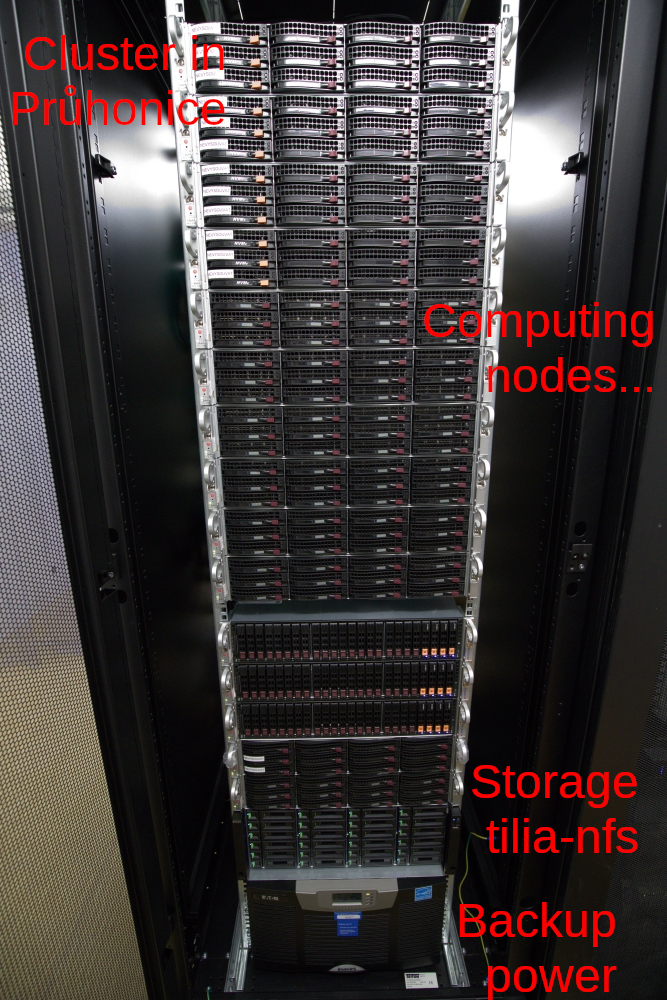
\includegraphics[height=6.5cm]{cluster_rack.jpg}
		\end{center}
	\end{multicols}
\end{frame}

\begin{frame}[allowframebreaks]{Distributed topology}
	\begin{itemize}
		\item \href{https://metavo.metacentrum.cz/}{MetaCentrum clusters} are distributed in various Czech cities (and institutions)
		\item Clusters use to have (at least small) storage array (accessible via \texttt{/storage/\ldots})
		\item There are special \href{https://du.cesnet.cz/en/infrastruktura_ulozist/start}{archive storages} (\href{https://du.cesnet.cz/cs/infrastruktura_ulozist/start}{česky}) in Jihlava, Ostrava and Plzeň
	\end{itemize}
	\begin{center}
		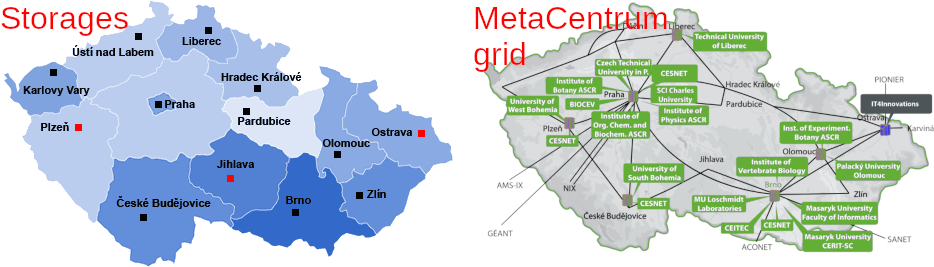
\includegraphics[width=\textwidth]{metacentrum_map.png}
	\end{center}
	\begin{itemize}
		\item Users have different quota on different arrays (depending on home organization etc.)
		\item There are 11 \href{https://wiki.metacentrum.cz/wiki/Frontend}{frontends} (\href{https://wiki.metacentrum.cz/wiki/Celni_uzel}{česky}) where user logs via SSH and prepare computing task for submission etc. (see further)
		\item Distributed topology might be bit confusing --- user has different home directory when logging to different frontends --- recommended is to use as few frontends and storages as possible
		\item Some special services (like \href{https://wiki.metacentrum.cz/wiki/OnDemand}{OnDemand}) start on particular storage (here \texttt{brno3})
		\item Generally, computing task loads data from selected storage and can start on any cluster
		\item Orientation is plenty of storages might be sometimes tricky --- ensure where you are and where your data are supposed to be
	\end{itemize}
\end{frame}

\subsection{Usage}

\begin{frame}{Basic workflow}
	\begin{center}
		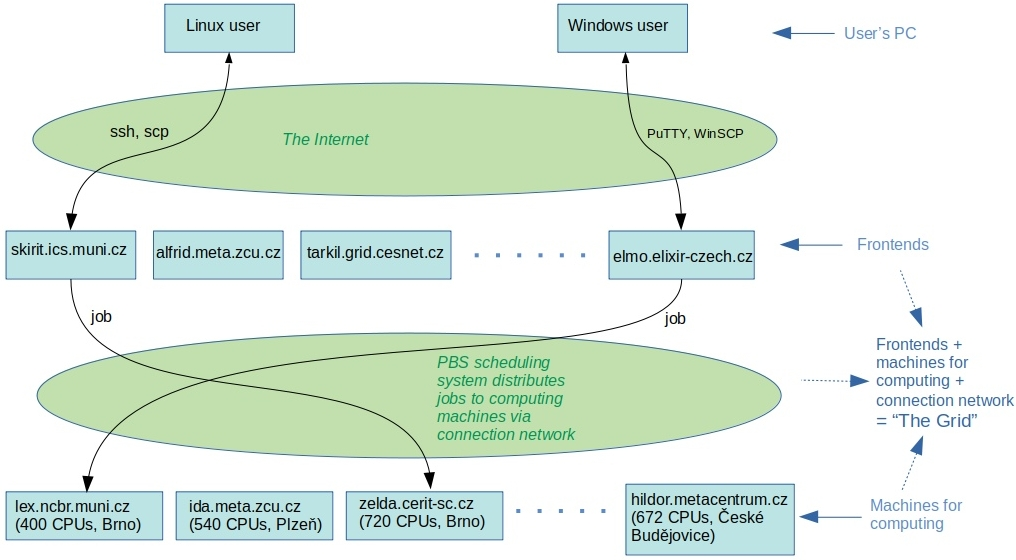
\includegraphics[height=5.5cm]{grid_graphics.jpg}
	\end{center}
	\begin{flushright}
		From \href{https://wiki.metacentrum.cz/wiki/Beginners_guide}{Beginners guide} (\href{https://wiki.metacentrum.cz/wiki/Pruvodce_pro_zacatecniky}{česky})
	\end{flushright}
\end{frame}

\begin{frame}[fragile]{MetaCentrum usage}
	\begin{enumerate}
		\item Transfer data into one of \href{https://wiki.metacentrum.cz/wiki/Working_with_data}{storages} (\href{https://wiki.metacentrum.cz/wiki/Prace_s_daty}{česky}) by e.g. \texttt{scp} from command line, \href{https://winscp.net/}{WinSCP} from Windows or \href{https://filezilla-project.org/}{FileZilla} from any OS
		\item Connect via SSH to select \href{https://wiki.metacentrum.cz/wiki/Frontend}{frontend} (\href{https://wiki.metacentrum.cz/wiki/Celni_uzel}{česky}). Same credentials are used for all frontends, for SSH login as well as file transmissions
		\item In home directory on the storage (accessed via frontend) prepare all needed data and non-interactive script to do the calculations
		\item Submit job using \texttt{qsub}. Tasks are not launched immediately, but submitted into queue and system decides when it will be launched
		\item Monitor job progress. Check results. Etc\ldots
	\end{enumerate}
	\begin{bashcode}
    # Login to selected server (tarkil is located in Prague)
    ssh USER@tarkil.metacentrum.cz
    # Continue as in any other command line...
    qsub ... # Submit the job (see later)
	\end{bashcode}
\end{frame}

\begin{frame}{File transfers to MetaCentrum}
	\begin{multicols}{2}
		\begin{itemize}
			\item Graphical applications: e.g. \href{https://filezilla-project.org/}{FileZilla} or most of Linux file managers
			\item Protocol is SSH/SSH2/SFTP/SCP, port 22, server is selected \href{https://wiki.metacentrum.cz/wiki/NFS4_Servery}{storage} address --- if possible, select any and keep using it
			\item All servers (storages, frontends, computing nodes) are accessible under domain \texttt{*.metacentrum.cz} --- e.g. \texttt{tarkil.grid.cesnet.cz} is same as \texttt{tarkil.metacentrum.cz}
			\item See slide \ref{transfers} and following to command-line transfers of files
		\end{itemize}
		\begin{center}
			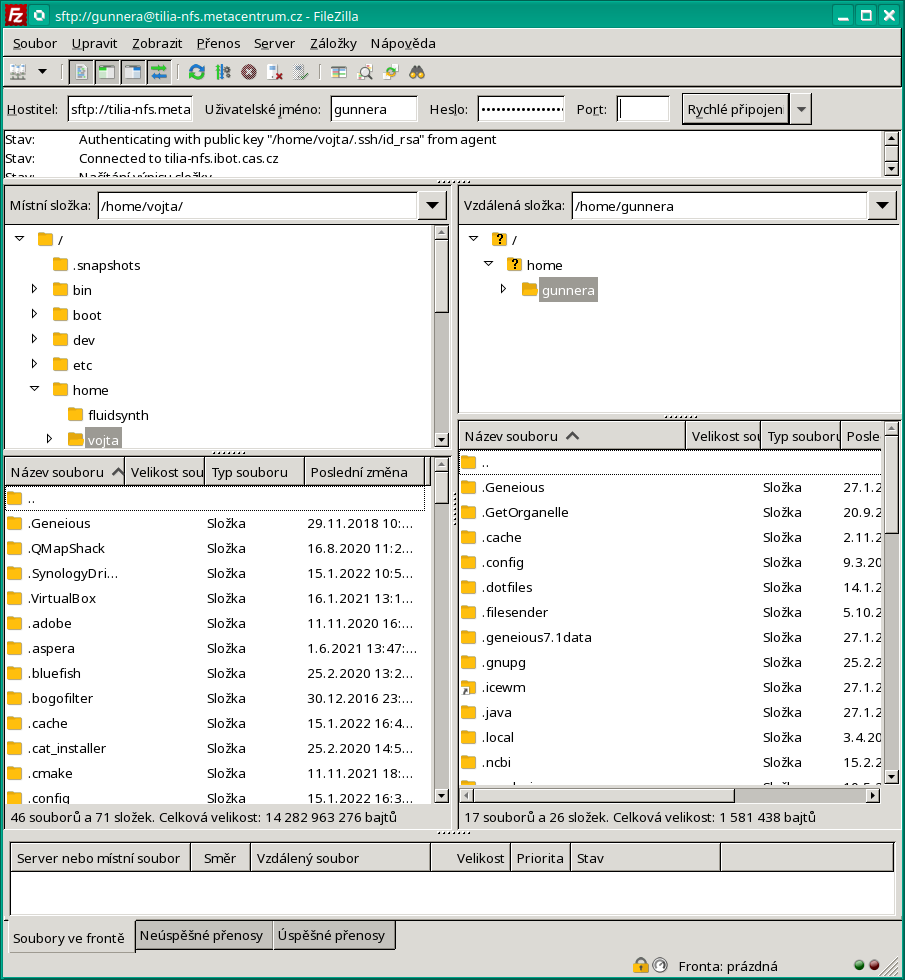
\includegraphics[height=6.5cm]{filezilla.png}
		\end{center}
	\end{multicols}
\end{frame}

\subsection{Tasks}

\begin{frame}[fragile]{Basic skeleton of script running tasks I}
	\begin{bashcode}
    #!/bin/bash
    # Modify the script according to your needs!
    # Set data directories
    WORKDIR="my_data_dir" # Or something else
    DATADIR="/storage/XXX/home/$LOGNAME" # Or other storage
    # There is e.g. directory /storage/praha1/home/gunnera/my_data_dir
    # containing all the data needed for calculations
    # Clean-up of SCRATCH (it is temporal directory created by server) - the
    # commands will be launched on the end when the job is done
    trap 'clean_scratch' TERM EXIT
    trap 'cp -a "${SCRATCHDIR}" "${DATADIR}"/ && clean_scratch' TERM
    # Change working directory - script goes to the directory where
    # calculations are done
    cd "${SCRATCHDIR}"/ || exit 1 # If it fails, exit script
    # Prepare the task - copy all needed files from working directory into
    # particular computer which will finally do the calculations
    # Ends on following slide...
	\end{bashcode}
\end{frame}

\begin{frame}[fragile]{Basic skeleton of script running tasks II}
	\begin{bashcode}
    # ...begins on previous slide; copy data - if it fails, exit
    cp -a "${DATADIR}"/"${WORKDIR}"/* "${SCRATCHDIR}"/ || exit 1
    # Prepare calculations - load required application modules
    # See https://wiki.metacentrum.cz/wiki/Kategorie:Applications
    # Every application module is loaded by "module add XXX"
    module add parallel # In this (example) case GNU Parallel and MrBayes
    module add mrbayes-3.2.6
    # Launch the analysis - calculate MrBayes for multiple files
    # Note Parallel will distribute task among 8 CPU threads (-j 8), so that
    # qsub must in this case contain select=1:ncpus=8 (see further)
    find . -name "*.nexus" -print | parallel -j 8 'mb {} | tee {.}.log'
    # Copy results back to $DATADIR directory
    cp -a "${SCRATCHDIR}" "${DATADIR}"/ || export CLEAN_SCRATCH='false'
    # This is all needed, the script is ready to be launched...
    exit
	\end{bashcode}
	\begin{itemize}
		\item Make \texttt{metacentrum.sh} executable and modify it to fit your needs\ldots
		\item If it was written on Windows, convert EOL (and encoding, slide~\ref{eolencoding})\ldots
	\end{itemize}
\end{frame}

\begin{frame}[fragile]{Launching of tasks}
	\begin{itemize}
		\item See \href{https://wiki.metacentrum.cz/wiki/Beginners_guide}{beginners guide} (\href{https://wiki.metacentrum.cz/wiki/Pruvodce_pro_zacatecniky}{česky}) and \href{https://wiki.metacentrum.cz/wiki/Categorized_list_of_topics}{list of topics} (\href{https://wiki.metacentrum.cz/wiki/Rozcestnik}{česky})
		\item Personal view \url{https://metavo.metacentrum.cz/pbsmon2/person} has nice overview of available resources and tasks and allows comfortable construction of submission command
	\end{itemize}
	\vfill
	\begin{bashcode}
    # We will run up to 5 days (120 hours), require one physical computer
    # with 8 CPU threads, 24 GB of RAM, 10 GB of disk space and we get all
    # information mails (for abort, beginning, exit)
    qsub -l walltime=120:0:0 -l select=1:ncpus=8:mem=24gb:scratch_local=10gb \
      -m abe metacentrum.sh
    # Check how the task is running (above web) and
    qstat -u $USER # Information about $USER's jobs (queued and running)
    qstat 123456789 # The task ID is available from commands above or mail
    qstat -f 123456789 # Print a lot of details
    qdel 123456789 # Terminate scheduled or running task
    qextend 123456789.meta-pbs.metacentrum.cz 12:0:0 # Prolong walltime (12 h)
	\end{bashcode}
\end{frame}

\begin{frame}[fragile]{Key MetaCentrum commands}
	\begin{itemize}
		\item MetaCentrum is \enquote{just} normal Linux server --- work there as on any other Linux system
		\item Command \texttt{module} loads/unloads selected \href{https://wiki.metacentrum.cz/wiki/Kategorie:Applications}{application}
		\item Tasks (BASH scripts) are submitted for computing by \texttt{qsub} --- the script must copy the data into \texttt{\$SCRATCHDIR} and do all calculations there
		\begin{itemize}
			\item It has plenty of options how to specify requirements (see next slide and \href{https://wiki.metacentrum.cz/wiki/About_scheduling_system}{help})
		\end{itemize}
		\item Queued and running jobs can be seen by \texttt{qstat -u \$USER} (\texttt{qstat} has much more options) and any job can be terminated by \texttt{qdel 123456789} (number from \texttt{qstat})
	\end{itemize}
	\vfill
	\begin{bashcode}
    module add <TAB><TAB> # Load some module
    module rm XXX # Unload selected module
    module list # List of currently loaded modules
    qsub ... # Submit task for computing - select any parameters needed
    qstat -u $USER # See $USER's running and queued jobs
    qdel 123456789 # Termite task (number from qstat)
	\end{bashcode}
\end{frame}

\begin{frame}[allowframebreaks]{Scheduling details}
	\begin{itemize}
		\item Specify needed time
		\begin{itemize}
			\item Always \texttt{hours:minutes:seconds}, so e.g. for 4~weeks use \texttt{-l~walltime=672:0:0} (28~$\cdot$~24), for two days and 12 hours \texttt{-l~walltime=60:0:0}
			\item User may extend it with \texttt{qextend} (see \texttt{qextend info}), otherwise \href{mailto:meta@cesnet.cz}{ask support} (write them in advance)
		\end{itemize}
		\item Ask for as much RAM as you need (e.g. \texttt{-l~mem=8gb} to request 8~GB)
		\begin{itemize}
			\item If the task is going to require more, than allowed, system kills it\ldots
			\item If user doesn't use all required RAM, the system temporarily lowers priority for future tasks (RAM is limiting resource, do not waste it)
			\item It can be hard to estimate (no easy general advice to estimate needs for particular task) --- do some experiment and see how your application behaves with your data\ldots
		\end{itemize}
		\item Disk space is relatively free resource, user can ask more to have some reserve (e.g. \texttt{-l~scratch\_local=10gb} to request 10~GB)
		\item Specify how many physical computer(s) you are going to use (e.g. \texttt{-l~select=1} for one machine) and number of CPU threads on each machine (e.g. \texttt{-l~select=1:ncpus=8} for 1~machine with 8~cores or \texttt{-l~select=2:ncpus=4} for 2~machines, each with 4~CPU threads)
		\begin{itemize}
			\item It use to be necessary to specify correct number of threads for the application (e.g. \texttt{parallel -j 4}) --- the application sees all CPUs on the machine, but can't use them
			\item If the application consumes less than required, the system temporarily lowers priority for future tasks, if it try to use more, it will be very slowed down or killed by the server
			\item If using more physical machines, ensure correct settings of e.g. MPI (see documentation for respective software you are using)
		\end{itemize}
		\item If requesting e-mails (e.g. \texttt{-m abe} to get mail about abort, beginning and exit of the task) and submitting plenty of tasks by some script, it can result in plenty of mails\ldots
		\item Every user has certain \href{https://metavo.metacentrum.cz/pbsmon2/users/}{priority} increased by \href{https://wiki.metacentrum.cz/wiki/Usage_rules/Acknowledgement}{acknowledgments} (\textbf{it's mandatory to acknowledge MetaCentrum when using it}) in publications to MetaCentrum, and lowered by intensive usage of the service (the usage is calculated from past month)
		\item After submission of the task, check in \href{https://metavo.metacentrum.cz/pbsmon2/queues/jobsQueued}{the queue} in which state it is --- sometimes it can't start because of impossible combination of requested resources or so
		\item User can \href{https://metavo.metacentrum.cz/pbsmon2/nodes/physical}{check load of machines}
		\item For more options read \url{https://wiki.metacentrum.cz/wiki/About_scheduling_system}
		\begin{itemize}
			\item Request special CPU (AMD, graphical,~\ldots), e.g. CPU with AVX2 \texttt{-l~select=cpu\_flag=avx2}
			\item SSD local storage (e.g. \texttt{-l~scratch\_ssd=1gb})
			\item Request particular location,~\ldots
			\item \url{https://metavo.metacentrum.cz/pbsmon2/qsub_pbspro} helps with preparation of \texttt{qsub} command
		\end{itemize}
	\end{itemize}
\end{frame}

\begin{frame}{Common problems with launching the tasks}
	\begin{itemize}
		\item Script fails because of wrong PATH or missing file --- ensure all needed files are transferred and applications receive correct paths
		\begin{itemize}
			\item Rather do not use absolute paths (starting with \texttt{/}) --- only relative
		\end{itemize}
		\item Not all required applications are correctly loaded
		\begin{itemize}
			\item Check \href{https://wiki.metacentrum.cz/wiki/Kategorie:Applications}{wiki} and load all needed applications
			\item Names of binaries are sometimes little bit different --- contain names of versions, etc.
		\end{itemize}
		\item Estimation of time needed to run the task
		\begin{itemize}
			\item No really good solution\ldots
			\item Make some trials and try to estimate\ldots
			\item There are very different CPUs available (with different speeds) --- it is possible to require particular CPU type (but it reduces number of available nodes\ldots)
		\end{itemize}
		\item Problems with CPU and memory
		\begin{itemize}
			\item Hard to estimate\ldots
			\item Some applications allow setting number of CPU threads --- check documentation
			\item If using Java application, it often helps to request one more CPU thread for Java itself
			\item Limiting memory is problematic, e.g. Java allows \texttt{java -Xmx8g -jar \ldots}, some applications also --- check documentation
		\end{itemize}
	\end{itemize}
\end{frame}

\begin{frame}[fragile]{Get to task's working directory}
	\begin{itemize}
		\item Go to \url{https://metavo.metacentrum.cz/pbsmon2/person} and click to list of your tasks and click to selected task
		\item Search for information \textbf{exec\_host} (address of node doing the task) and \textbf{SCRATCHDIR} (temporal directory for all data and results)
		\item Sometimes one needs to monitor task progress or influence it
		\item It is not possible to directly modify running task, but at least check (and possibly modify) input data and see outputs
	\end{itemize}
	\begin{bashcode}
    # From any MetaCentrum frontend login to respective node running the task
    ssh exec_host # No need to specify user name; e.g. mandos9
    # Go to SCRATCH directory
    cd SCRATCHDIR # e.g. /scratch/USER/job_1234567.arien-pro.ics.muni.cz/
    # There are working data of currently running task...
    # Check whatever you need...
	\end{bashcode}
\end{frame}

\begin{frame}{Running R tasks on MetaCentrum}
	\begin{itemize}
		\item There are only some R packages, to get more create own package library and use it in scripts (see e.g. \texttt{/software/R/4.0.0/gcc/lib/R/library/})
		\item \alert{Be careful about paths!}
		\item In the \texttt{metacentrum.sh} script load R \texttt{module add R-4.0.0-gcc} and start there R script as usually \texttt{R CMD BATCH script.r}
	\end{itemize}
	\begin{enumerate}
		\item Login to selected front node via SSH
		\item Create somewhere new directory for R packages \texttt{mkdir rpkgs} (or use default \texttt{$\sim$/R/})
		\item Start R \texttt{R} and install \textbf{all} R packages needed for the task --- install them into the \texttt{rpkgs} directory \texttt{install.packages(pkgs=\ldots, lib="rpkgs")}
		\item In the R script \texttt{*.r} load the packages from the \texttt{rpkgs} directory \texttt{library(package=\ldots, lib.loc="/storage/\ldots/rpkgs")}
		\item Ensure all needed outputs are saved from the R script
	\end{enumerate}
\end{frame}

\begin{frame}[fragile]{Interactive tasks}
	\begin{bashcode}
    # Secure we can log off in the meantime
    screen # Or tmux
    # Again launch qsub according to actual needs
    # Note "-I" for interactive session and missing script name
    qsub -I -l walltime=1:0:0 -l select=1:ncpus=1:mem=1gb:scratch_local=1gb
    # Wait for job to start... User automatically gets to the computing node
    cd $SCRATCHDIR # Go to $SCRATCHDIR - work there
    # After we get the interactive task, we are on new server
    # Do needed work...
    # When done, be sure to copy results to the storage
    hostname # See where we are - we can connect to that server directly
    ssh USER@given.server.cz # User name and password are the same
                             # Server address is output from "hostname"
    # When you logout, the task is done (use screen to secure connection)
	\end{bashcode}
	\vfill
	\begin{itemize}
		\item Work as on normal Linux server\ldots
		\item With \texttt{screen} we can disconnect as usually and let tasks run in background
	\end{itemize}
\end{frame}

\subsection{}

\begin{frame}{MetaCentrum task}
	\begin{enumerate}
		\item Upload to any MetaCentrum fronted files \texttt{metacentrum\_oxalis.sh} and \texttt{oxalis\_assembly\_6235.aln.fasta} from \texttt{scripts\_data}.
		\item See \texttt{metacentrum\_oxalis.sh}, be sure you know what it is doing, that you understand every command there.
		\item If needed, edit \texttt{metacentrum\_oxalis.sh} (e.g. correct paths).
		\item Submit the task via \texttt{qsub}.
		\item Monitor the task with \texttt{qstat}.
		\item Login with SSH to computing node where the task is running, go to \texttt{\$SCRATCHDIR} and see its progress. Look at output of \texttt{ps ux}. What does it say?
		\item Wait for the task to be done and explore output (e.g. open the \texttt{treefile} in \href{http://tree.bio.ed.ac.uk/software/figtree/}{FigTree}).
		\item If you encounter any error, try to find its source and fix it.
	\end{enumerate}
\end{frame}

\subsection{Graphical connection}

\begin{frame}[fragile]{Graphical interactive task}
	\begin{itemize}
		\item See \url{https://wiki.metacentrum.cz/wiki/Remote_desktop}
	\end{itemize}
	\begin{bashcode}
    screen # Secure we can log off in the meantime
    # Again launch qsub according to actual needs
    # Note "-I" for interactive session and missing script name
    qsub -I -l walltime=1:0:0 -l select=1:ncpus=1:mem=1gb:scratch_local=1gb
    # Wait for job to start... User automatically gets to the computing node
    # After we get the interactive task, we are on new server
    module add gui # We need to add GUI module
    gui start --ssh # Start GUI (see above link for details)
    gui info # Print information about running VNC sessions
	\end{bashcode}
	\begin{itemize}
		\item Download and install \href{https://www.tightvnc.com/}{TightVNC} (Windows installer or Java Viewer)
		\item Work as on normal Linux desktop (ensure to work in \texttt{\$SCRATCHDIR})\ldots
		\item It provides limited amount of resources, not suitable for big tasks
	\end{itemize}
\end{frame}

\begin{frame}{Running VNC}
	\begin{center}
		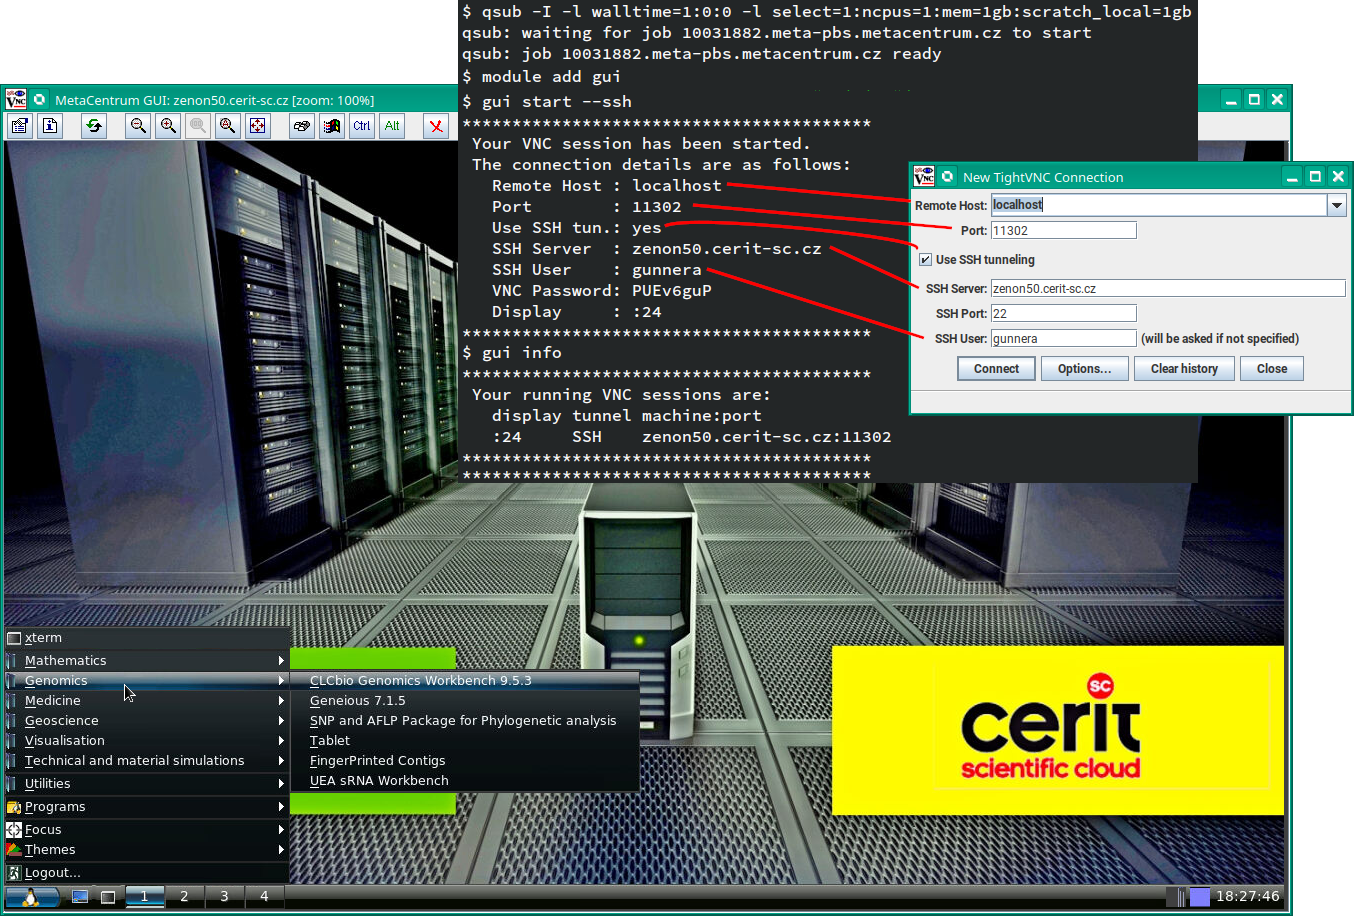
\includegraphics[height=6.5cm]{vnc.png}
	\end{center}
\end{frame}

\subsection{Archive data storage}

\begin{frame}{CESNET archive data storage}
	\begin{itemize}
		\item Read documentation \url{https://du.cesnet.cz/} and connection instructions \url{https://du.cesnet.cz/en/navody/sluzby/start} (\href{https://du.cesnet.cz/cs/navody/sluzby/start}{česky})
		\item Generally, it is possible to connect via FTPS, NFS, SAMBA (Windows network drive), SCP/SFTP or SSH --- more options how to get to same resource
		\item See slide~\ref{CESNET} for general information and \ref{transfers} for connecting information
		\item After logging via SSH, it is possible to work as on any other server
		\item Users get information about selected storage location and paths after registration (there are several locations, user get space on one of them)
		\begin{itemize}
			\item There are plenty of storages, be careful where you are connecting to and what is the path --- e.g. when connecting directly to \texttt{du4.cesnet.cz}, paths are \texttt{/tape\_tape/\ldots}, from any other MetaCentrum node \texttt{\textbf{/storage/ostrava2-archive}/tape\_tape/\ldots}
		\end{itemize}
		\item All storage locations are accessible from any MetaCentrum front node via directories in \texttt{/storage} (e.g. \texttt{/storage/ostrava2-archive/tape\_tape/VO\_\ldots})
	\end{itemize}
\end{frame}

\begin{frame}[fragile]{Shared space on CESNET data storage}
	\begin{itemize}
		\item Users \href{https://du.cesnet.cz/en/uzivatelska_podpora/start}{can ask} (\href{https://du.cesnet.cz/cs/uzivatelska_podpora/start}{česky}) for creation of shared space
		\begin{itemize}
			\item Normally, the space is private only for particular user
			\item Groups allow more users to share data
			\item Data storage admins will instruct users regarding locations, paths, permissions, etc. (it is specific for each case)
		\end{itemize}
		\item Users must carefully set permissions!
		\begin{itemize}
			\item Sharing is done by specific UNIX group
			\item Users must set group ownership to particular group and permissions e.g. 770 for directories and 660 for files to avoid access of any other users
			\item All members of the group must be able to manipulate the data
		\end{itemize}
	\end{itemize}
	\vfill
	\begin{bashcode}
    # Change group ownership to XXX
    chgrp -R XXX /tape_tape/VO_XXX 2>/dev/null
    # ("-R" to modify also subdirectories; "2>/dev/null" to discard errors)
    # Set correct permissions to directories and files
    find /tape_tape/VO_XXX -type d -exec chmod 770 {} \; 2>/dev/null
    find /tape_tape/VO_XXX -type f -exec chmod 660 {} \; 2>/dev/null
	\end{bashcode}
\end{frame}

\subsection{More services}

\begin{frame}{OnDemand}{Applications in web browser}
	\begin{itemize}
		\item It allows to run selected interactive applications in web browser
		\item See \url{https://wiki.metacentrum.cz/wiki/OnDemand} and \url{https://ondemand.cerit-sc.cz/}
		\item Applications start in \texttt{/storage/brno3-cerit/home/\$USER/} --- ensure to have everything needed there
	\end{itemize}
	\begin{center}
		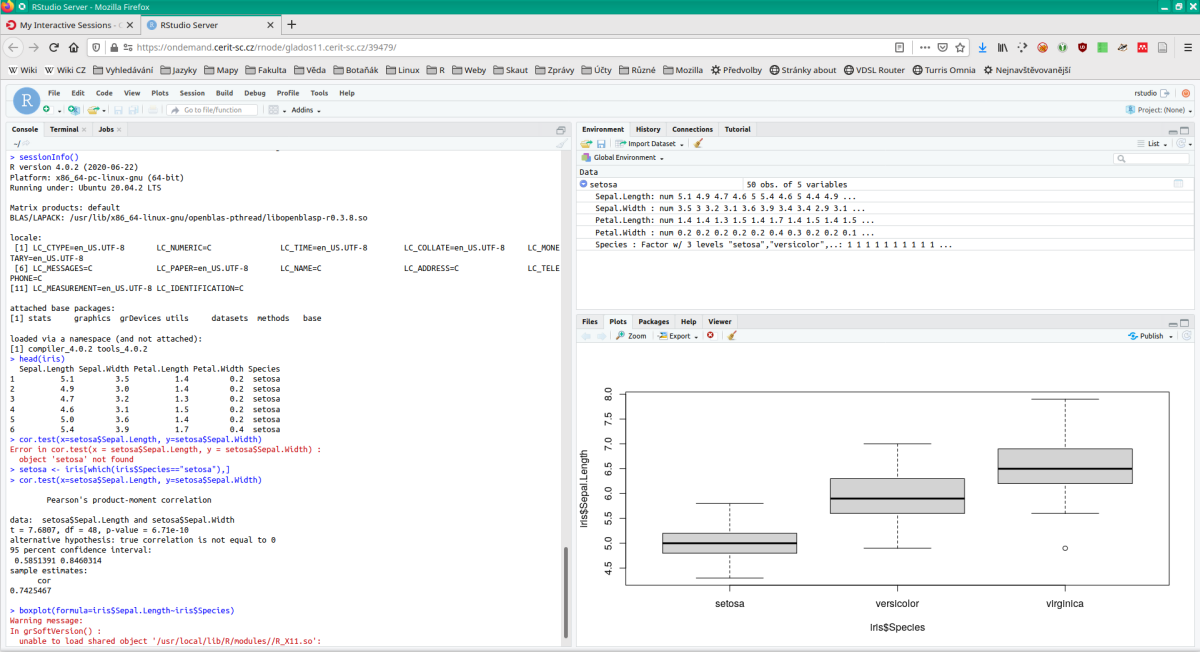
\includegraphics[height=3.5cm]{rstudio_ondemand.png}
	\end{center}
\end{frame}

\begin{frame}{Jupyter Notebook}
	\begin{multicols}{2}
		\begin{itemize}
			\item Web service allowing to record code as well as its output for languages like BASH, R, Python,~\ldots
			\item Convenient for recording and sharing code, interactive work,~\ldots
			\item Use \href{https://wiki.metacentrum.cz/wiki/Jupyter_for_MetaCentrum_users}{Jupyter Hub} for MetaCentrum users
			\begin{itemize}
				\item Data are in \texttt{/storage/brno2/home/USER/}
			\end{itemize}
			\item \href{https://wiki.metacentrum.cz/wiki/Jupyter_notebook}{Available} also as part of OnDemand (previous slide), or bit experimental \href{https://hub.cerit-sc.cz/}{CERIT hub}, which allows to select custom storage and also custom docker image (see \href{https://docs.cerit.io/docs/jupyterhub.html}{documentation})
		\end{itemize}
		\begin{center}
			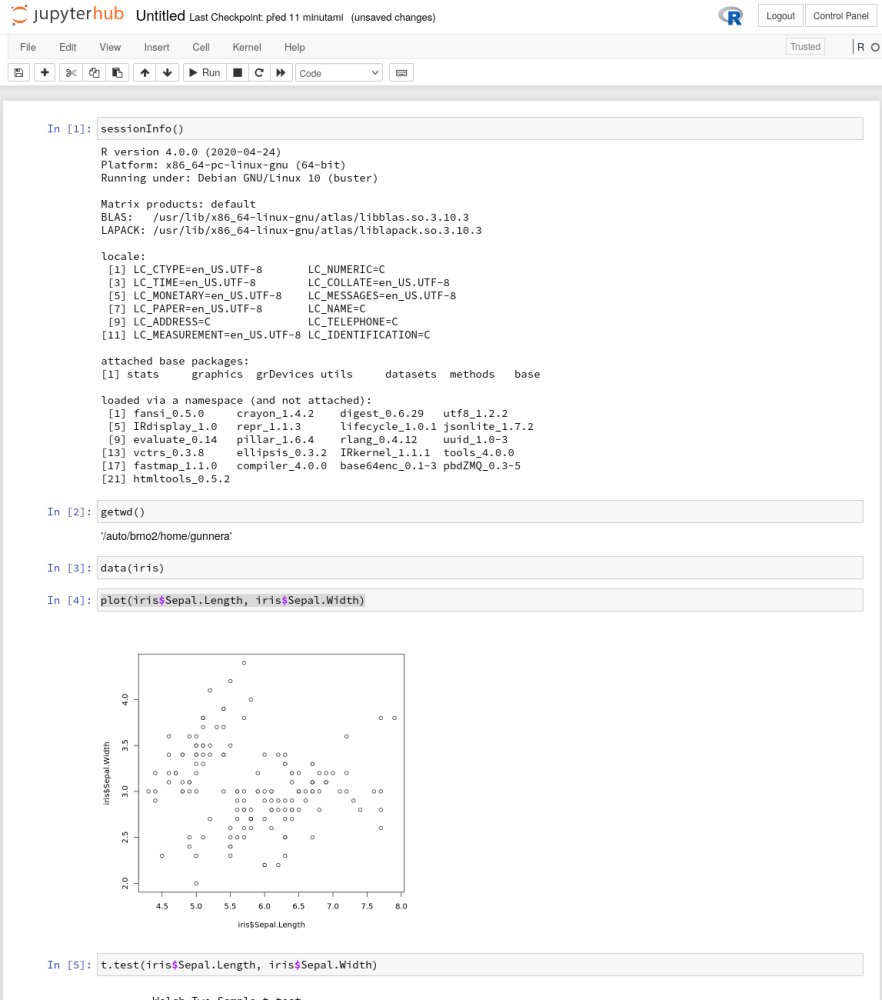
\includegraphics[height=6.5cm]{jupyter.png}
		\end{center}
	\end{multicols}
\end{frame}

\begin{frame}{MetaCentrum cloud}
	\begin{itemize}
		\item MetaCentrum \href{https://wiki.metacentrum.cz/wiki/Kategorie:Clouds}{cloud} (\href{https://wiki.metacentrum.cz/wiki/Kategorie:Cloudy}{česky}) allows to run complete Linux distribution (Debian, CentOS,~\ldots), where you can install any software, like on any other computer
		\item Useful e.g. for various testing or applications with very special requirements
		\item Go to \url{https://cloud.metacentrum.cz/} and see \href{https://docs.cloud.muni.cz/}{documentation}
		\item Login to running virtual machine requires SSH keys to be set up, access is normally via SSH
		\item Users must have knowledge about Linux administration and follow all security best-practices
		\item Setting up more than one virtual machine requires good knowledge about Linux networking (user has single public IP address)
	\end{itemize}
\end{frame}

\section{Git}

\begin{frame}{Git}
	\begin{multicols}{2}
		\vfill
		\tableofcontents[currentsection, sectionstyle=show/hide, hideothersubsections]
		\columnbreak
		\begin{center}
			
\includegraphics[height=5.5cm]{git_xkcd.png}
		\end{center}
		\begin{flushright}
			\url{https://xkcd.com/1597/}
		\end{flushright}
	\end{multicols}
\end{frame}

\subsection{Git principle}

\begin{frame}[allowframebreaks]{Git and version control}
	\begin{itemize}
		\item \href{https://git-scm.com/}{Git} is \href{https://en.wikipedia.org/wiki/Version_control}{version controlling} (\href{https://cs.wikipedia.org/wiki/Verzov\%C3\%A1n\%C3\%AD}{česky}) system (nowadays the most common) --- it traces changes among all versions --- absolutely crucial for any software development
		\item Older (nowadays not so common) version controlling systems is Subversion (SVN), there are many more (Bazaar, Mercurial,~\ldots)
		\item Probably the best textbook for Git is \href{https://git-scm.com/book/en/v2}{Chacon's Pro Git}
		\begin{itemize}
			\item Dostupná i~\href{https://git-scm.com/book/cs/v2}{česky} (včetně \href{https://knihy.nic.cz/\#ProGit}{prvního vydání})
		\end{itemize}
		\item Changes and their history is stored in repository (local or network, shared or private) --- it is possible to view any historical state and differences between any versions
		\item It is possible to trace who and when did what
		\item Branching and merging of branches helps with making of big changes
		\begin{itemize}
			\item When new branch is created, it contains copy of current state
			\item User selects in which branch she/he is working, the branches are diverging, user can commit in every branch independently
			\item Commits in various branches can be compared and branches can be merged again
			\item Key feature of Git --- branches are useful when user starts to work on any big change in the project (the \enquote{main} part is intact while developers can freely work on major change)
		\end{itemize}
		\item Users work on a project in some directory as usually and from time to time commit local changes to stagging (temporal area) and then push them to remote or local repository (directory storing all Git history of particular project, can be anywhere)
		\item Every commit is checkpoint in the history
		\begin{itemize}
			\item Can be tagged (named), e.g. particular released version of software, or project stage
			\item User can compare any two commits or commit and current state
		\end{itemize}
		\item Stagging area serves as local \enquote{container} of changes to be pushed to central Git repository (or to be modified, discarded)
		\item Central repository keeps whole history of the project
		\begin{itemize}
			\item Every user has full copy of the central Git repository --- can be large
		\end{itemize}
		\item Git was developed by Linus to trace development of Linux kernel, now it is probably the most used version control tool, used also by Microsoft to trace development of Windows :-)
	\end{itemize}
\end{frame}

\begin{frame}{GitHub and others}
	\begin{itemize}
		\item \href{https://github.com/}{GitHub} is currently probably the most popular platform to host development of open-source projects, see \href{https://help.github.com/}{documentation}
		\item Probably second most common on-line service providing Git repository is \href{https://about.gitlab.com/}{GitLab}
		\begin{itemize}
			\item User can create an account on GitLab (as on GitHub), or download and install GitLab system on own server (like \href{https://sorbus.ibot.cas.cz/en/gitlab}{we did}, \href{https://sorbus.ibot.cas.cz/cs/gitlab}{česky})
		\end{itemize}
		\item \href{https://sourceforge.net/}{SourceForge} used to be more popular in the past, still harbours plenty of interesting projects
		\item Others are e.g. \href{https://bitbucket.org/}{Bitbucket}, \href{https://www.codebasehq.com/}{Codebase},~\ldots
		\item For on-line services, many tools are available only for paying customers
		\item All such services provide Git repositories accessible through standard tools (from command line, see further; or from some special application), through web browser
		\begin{itemize}
			\item Exact usage might differ from standard Git, check respective help pages first
		\end{itemize}
		\item Git repository can be easily hosted e.g. on any Linux server\ldots
	\end{itemize}
\end{frame}

\begin{frame}[fragile]{Git principles}
	\begin{multicols}{2}
		\begin{itemize}
			\item Three main areas
			\begin{enumerate}
				\item Working directory
				\item Staging (changes awaiting to be pushed to the repository)
				\item Git repository (remote/local)
			\end{enumerate}
			\item Everyone has whole repository and history --- very robust
			\item Flexible branches
			\begin{itemize}
				\item Very convenient
				\item Keeping work structured
				\item Separation of tasks
				\item Keeping more versions of the project
			\end{itemize}
			\item \alert{Homework:} play \href{https://ohmygit.org/}{Oh My Git!} to learn more and practice
		\end{itemize}
		\begin{center}
			\includegraphics[height=5cm]{git.png}
		\end{center}
		\begin{flushright}
			\begin{footnotesize}
				\href{https://git-scm.com/book/en/v2/Getting-Started-About-Version-Control}{https://git-scm.com/}, \href{https://nvie.com/posts/a-successful-git-branching-model/}{https://nvie.com/}
			\end{footnotesize}
		\end{flushright}
	\end{multicols}
\end{frame}

\subsection{Git basics}

\begin{frame}[fragile]{Working with Git --- start and sending changes}
	\begin{bashcode}
    # Create a new central repository (e.g. on a server) in empty directory
    git init --bare
    # Create a new repository for new project (in empty directory)
    git init # No need when cloning from existing repository
    # If you did not start by cloning, add connection to server
    git remote add origin <location> # Do only once on the beginning
    # <location> can be remote server or local path
    git remote add origin . # For repository within working directory
    # Or checkout (make a copy) of existing local or remote repository
    git clone /path/to/local/repository # Locally mounted repository
    git clone username@host:/path/to/remote/repository # Over SSH
    git clone https://github.com/V-Z/course-linux-command-line-bash-
      scripting-metacentrum.git # Clone from web, e.g. GitHub
    # Add files to trace with Git
    # Ignored files (or patterns) can be listed in .gitignore file
    git add <files> # Or "git add *"
    git status # See changed files, commits in stagging, etc.
	\end{bashcode}
\end{frame}

\begin{frame}[fragile]{Working with Git --- branching and getting changes}
	\begin{bashcode}
    # Commit changes to prepare them to send to repository
    git commit -m "Message..."
    # Push changes into the repository (regardless where it is)
    git push origin master # See further for selection of branches
    # Making new branch and switching to it
    git checkout -b NewFeature # Now we are in branch NewFeature
    # Switch back to branch master
    git checkout master # Generally, "git checkout <branch>"
    # Delete the branch (changes there are lost, must be in another branch)
    git branch -d NewFeature # Delete local branch
    git push origin --delete <branch> # Delete remote branch
    # New branch must be also pushed to the remote server
    git push origin <branch>
    # List branches (current is marked by asterisk on the beginning)
    git branch
    # Download news from central server (work of colleagues, etc.)
    git fetch # Downloaded to stagging, not applied yet to local files
	\end{bashcode}
\end{frame}

\begin{frame}[fragile]{Working with Git --- tags, logs and more}
	\begin{bashcode}
    # Update local repository to the newest version from central repository
    git pull # Fetch and merge remote changes (before commit)
    # Merge another branch into the current one
    git merge <branch>
    # In case of conflict, git shows editor and user must fix it manually
    git add <file with conflict> # Needed to re-add conflicting file
    # To see changes before merging
    git diff <source_branch> <target_branch>
    # Tagging e.g. milestones, released versions of software, etc.
    git tag <name> <commit id> # <name> can be custom, <commit id> from log:
    git log # Newest is on top, see also "git log --help"
    git log --graph --oneline --decorate --all # Full long log
    # Discard local changes for particular file
    git checkout --- <file>
    # Discard all local changes
    git fetch origin # Overwrite local changes
    git reset --hard origin/master # If local repository is broken...
	\end{bashcode}
\end{frame}

\begin{frame}[fragile]{Working with Git --- summary, settings and more}
	\begin{itemize}
		\item Basically repeat in \texttt{git} \texttt{add}, \texttt{commit} and \texttt{push} to get your work to the repository, and \texttt{fetch} and \texttt{pull} to download news from central repository
		\item \texttt{diff} to see local changes, \texttt{status} to see state
		\item \texttt{log} and \texttt{branch} show history and branches
		\item \texttt{branch}, \texttt{checkout} and \texttt{merge} for branching code and merging changes back to master (main) branch
	\end{itemize}
	\begin{bashcode}
    git diff # See changes in particular text files
    gitk # Graphical interface
    git config color.ui true # Set output to be colored
    git config format.pretty oneline # Nicer log output
    ~/.git # Contains user's settings, .git in every repository contains
           # data and settings for particular repository
           # Default behavior of Git can be heavily altered
	\end{bashcode}
\end{frame}

\subsection{}

\begin{frame}{Git tasks}
	\begin{enumerate}
		\item Clone over SSH repository \texttt{USER@vyuka.natur.cuni.cz:/home/dadaism} (use your credentials on the testing server) and go to \texttt{dadaism} directory.
		\item Add some text files, edit existing text files. Do not add images or another non-text files, do not add large files.
		\item Push your changes back to the repository.
		\item Fetch changes done by others.
		\item See history of changes, who did what, etc.
		\item Use at least \texttt{git} commands \texttt{clone},\texttt{diff}, \texttt{status}, \texttt{add}, \texttt{commit}, \texttt{push}, \texttt{fetch}, \texttt{pull}, \texttt{log} and \texttt{gitk}.
		\item You can try to play with branches --- \texttt{branch}, \texttt{checkout}, \texttt{merge}.
		\item Communicate with others to avoid conflicting edits.
	\end{enumerate}
\end{frame}

\section{Administration}

\begin{frame}{Administration}
	\tableofcontents[currentsection, sectionstyle=show/hide, hideothersubsections]
\end{frame}

% \begin{frame}{Btrfs and Snapper} % TODO Btrfs, Snapper
% 	\begin{itemize}
% 		\item 
% 	\end{itemize}
% \end{frame}

\subsection{System services}

\begin{frame}[fragile]{Managing system services}
	\begin{itemize}
		\item Different among distributions --- several main methods
		\item In Linux, most common is \href{https://wiki.freedesktop.org/www/Software/systemd/}{SystemD}, less common older init scripts and RC scripts
		\item macOS and various BSD and other systems have different methods
		\item Used to manage system services like networking, cron, web server, database,~\ldots
		\item \alert{Read documentation of your distribution first!}
		\item Most of actions require root authentication
		\item For SystemD there are also graphical managers (\href{https://doc.opensuse.org/documentation/leap/reference/html/book-reference/cha-systemd.html#sec-boot-runlevel-edit}{YaST}, \href{https://store.kde.org/p/1127873/}{Systemd-kcm} for KDE, \href{https://github.com/GuillaumeGomez/systemd-manager}{GTK Systemd Manager}, web-based \href{https://cockpit-project.org/}{Cockpit},~\ldots)
	\end{itemize}
	\vfill
	\begin{bashcode}
    # SystemD - huge amount of possibilities
    systemctl enable/disable/status/start/stop servicename # TAB helps
    # RC scripts
    rcservicename status/start/stop # TAB helps to select service
    # Init scripts
    /etc/init.d/servicename status/start/stop # TAB helps to select service
	\end{bashcode}
\end{frame}

\begin{frame}[fragile]{SystemD usage (few examples)}
	\begin{bashcode}
    # List installed services and their status
    systemctl list-units --type service
    # Enable/disable/see status/start/stop/restart/... service
    systemctl enable/disable/status/start/stop/restart servicename # TAB...
    # Show overridden config files after upgrade
    systemd-delta
    # Analyze boot time (how long does each service take to start)
    systemd-analyze blame # Text output
    systemd-analyze plot > filename.svg # Same in graphics
    # Log for particular service
    journalctl -u servicename
    # Last logged messages (press Ctrl+C to exit)
    journalctl -f
    # Log records since last boot
    journalctl -b
    # Time and date information and management
    timedatectl
	\end{bashcode}
\end{frame}

% \begin{frame}{Security} % TODO Security, antiviruses
% 	\begin{itemize}
% 		\item 
% 	\end{itemize}
% \end{frame}

\section{The End}

\begin{frame}{The End}
	\tableofcontents[currentsection, sectionstyle=show/hide, hideothersubsections]
\end{frame}

% \subsection{Switching to Linux} % TODO Switching
%
% \begin{frame}[allowframebreaks]{Brief list of applications to help to switch to Linux}
% 	\begin{itemize}
% 		\item 
% 	\end{itemize}
% \end{frame}

\subsection{Resources}

\begin{frame}[allowframebreaks]{Resources to learn to work in the terminal}
	\begin{itemize}
		\item openSUSE (general handbook) \url{https://doc.opensuse.org/documentation/leap/startup/html/book-startup/part-bash.html}
		\item Ubuntu (general handbook) \url{https://help.ubuntu.com/community/UsingTheTerminal}
		\item BASH full reference manual \url{https://www.gnu.org/software/bash/manual/} (advanced)
		\item Debian (general handbook) \url{https://www.debian.org/doc/manuals/debian-reference/ch01.en.html}
		\item Guide to Unix \url{https://en.wikibooks.org/wiki/Guide_to_Unix}
		\item BASH for beginners \url{https://tldp.org/LDP/Bash-Beginners-Guide/html/Bash-Beginners-Guide.html} (the site has plenty of good resources)
		\item Grymoire for UNIX wizards \url{https://www.grymoire.com/Unix/}
		\item Linux tutorial \url{https://ryanstutorials.net/linuxtutorial/}
		\item Getting Started with BASH \url{https://www.hypexr.org/bash_tutorial.php}
		\item Bash Guide \url{https://mywiki.wooledge.org/BashGuide}
		\item TutorialKart \url{https://www.tutorialkart.com/bash-shell-scripting}
		\item Česky
		\begin{itemize}
			\item Učebnice Linuxu \url{https://www.abclinuxu.cz/ucebnice}
			\item Příkazová řádka Ubuntu \url{https://wiki.ubuntu.cz/syst\%C3\%A9m/p\%C5\%99\%C3\%ADkazov\%C3\%A1_\%C5\%99\%C3\%A1dka/termin\%C3\%A1l}
			\item Příkazová řádka Fedory \url{https://wiki.mojefedora.cz/domains/wiki.mojefedora.cz/doku.php?id=navody:prirucka:prompt}
			\item Johančiny Pohádky z~příkazové řádky \url{https://eldar.cz/kangaroo/binarni-sxizofrenie/johanka-pohadky-z-prikazove-radky.html}
		\end{itemize}
	\end{itemize}
\end{frame}

\begin{frame}[allowframebreaks]{How to ask for help}
	\label{howtoask}
	\begin{itemize}
		\item \alert{Never ever} ask simple silly lazy questions you can quickly find in manual or web
		\item People on mailing lists and forums respond volunteerly in their spare free time --- do not waste it --- be polite, brief and informative
		\item Imagine you should answer --- which information do you need?
		\item Be as specific and exact as possible
		\begin{itemize}
			\item Write \alert{exactly} what you did (\enquote{It doesn't work!} is useless\ldots)
			\item Copy/paste your commands and their output, especially error messages --- they are keys to solve the problem
			\item Try to search web for the error messages (or their parts)
			\item Try to provide minimal working example --- add at least part of your data (if applicable) so that the problem is reproducible
			\item Specify name and version of distribution and of the problematic software
		\end{itemize}
		\item \textbf{OSS is free as freedom of speech --- not as free beer!}
		\begin{itemize}
			\item As soon as you don't pay for support, you can't blame anyone for lack of responses
			\item Most of software we use to process our data is provided under \enquote{best effort}, without warranty\ldots
			\item Plenty of scientific software is not written by professional programmers, authors often do not foresee everything what could happen and they could have troubles wehn fixing reported issues\ldots
			\item There are plenty of reasons some software doesn't work --- usage/data author didn't expect, unsupported version of operating system, author's mistake, user's mistake, unexpected interaction with another software,~\ldots
			\item Authors wish their software to be useful --- constructive feedback, reporting bugs and wishes is welcomed, but it must be provided in the way useful for the developer
		\end{itemize}
		\item Try to find the best place to ask your question --- specific forum for particular distribution or software use to be the best option
		\item Learning command line is like learning foreign language --- it takes time\ldots
		\item \alert{Reading documentation is not wasting of time!}
	\end{itemize}
\end{frame}

\begin{frame}[allowframebreaks]{Main general fora}
	\begin{block}{Question must have certain form!}
			Before asking, \alert{ensure your question is in answerable form} (previous slides).
		\begin{itemize}
			\item Sloppily asked question can't be answered at all\ldots
			\item Check documentation, manuals and search the Internet before asking
		\end{itemize}
	\end{block}
	\begin{itemize}
		\item Probably the best are fora from StackExchange \url{https://stackexchange.com/sites}
		\item General forum for programmers \url{https://stackoverflow.com/}
		\item UNIX forum \url{https://unix.stackexchange.com/}
		\item Forum for administrators \url{https://superuser.com/}
		\item Questions mainly (not only) related to servers \url{https://serverfault.com/}
		\item \href{https://www.startpage.com/}{Uncle Google} is your friend here (\textit{\enquote{how to XXX in BASH/Linux}})\ldots
		\item Bioinformatics and related topics is discussed on \href{https://www.biostars.org/}{Biostars} and \href{https://bioinformatics.stackexchange.com/}{StackExchange}
		\item Do not hesitate to ask on the forum or contact developers, preferably through some public forum or mailing list, they usually respond quickly and helpfully\ldots{ }--- they wish their software to be working and useful
		\item Plenty of bigger projects have their own web fora or e-mail conferences --- search for it to ask on right place
		\item In Linux/OSS world, e-mail conferences are sometimes more popular, than web forums or various social networks --- try them
		\item If you find a~bug, report it according to instructions given by the project
		\item Plenty of software packages have bug (issue) trackers (e.g. on GitHub) to report any problem with the software and discuss --- search them on software homepage
		\item Programming languages like R or Python have their own discussion fora, commonly specific for particular field
	\end{itemize}
\end{frame}

\begin{frame}{openSUSE}
	\begin{itemize}
		\item Homepage \url{https://www.opensuse.org/}
		\item Wiki (knowledge base) \url{https://en.opensuse.org/Main_Page}
		\item Documentation \url{https://doc.opensuse.org/}
		\item News \url{https://news.opensuse.org/}, blogs \url{https://planet.opensuse.org/}
		\item Forums \url{https://forums.opensuse.org/}
		\item Mailing lists \url{https://lists.opensuse.org/}
		\item Community \url{https://opensuse-community.org/}, short community guide \url{https://opensuse-guide.org/}
	\end{itemize}
\end{frame}

\begin{frame}{Debian, Ubuntu, Linux Mint and derivatives}
	\begin{itemize}
		\item Debian \url{https://www.debian.org/}
		\begin{itemize}
			\item Documentation, wiki \url{https://wiki.debian.org/}
			\item Support \url{https://www.debian.org/support}
		\end{itemize}
		\item Ubuntu \url{https://ubuntu.com/}
		\begin{itemize}
			\item Support \url{https://ubuntu.com/support}
			\item Ask Ubuntu (probably the best forum) \url{https://askubuntu.com/}
			\item Forum \url{https://ubuntuforums.org/}
			\item Documentation \url{https://help.ubuntu.com/}
			\item Kubuntu \url{https://kubuntu.org/}
			\item Kubuntu forum \url{https://www.kubuntuforums.net/}
			\item Xubuntu \url{https://xubuntu.org/}
			\item Lubuntu \url{https://lubuntu.me/}
		\end{itemize}
		\item Linux Mint \url{https://www.linuxmint.com/}
		\begin{itemize}
			\item Documentation \url{https://www.linuxmint.com/documentation.php}
			\item Forums \url{https://forums.linuxmint.com/}
		\end{itemize}
	\end{itemize}
\end{frame}

\begin{frame}{Fedora}
	\begin{itemize}
		\item Homepage \url{https://getfedora.org/}
		\item Communication and help overview \url{https://fedoraproject.org/wiki/Communicating_and_getting_help}
		\item Wiki \url{https://fedoraproject.org/wiki/Fedora_Project_Wiki}
		\item Official forum \url{https://ask.fedoraproject.org/}
		\item Documentation \url{https://docs.fedoraproject.org/}
		\item Community forum \url{https://fedoraforum.org/}
	\end{itemize}
\end{frame}

\begin{frame}{GNOME, KDE and XFCE}
	\begin{itemize}
		\item GNOME \url{https://www.gnome.org/}
		\begin{itemize}
			\item Help for users \url{https://help.gnome.org/users/}
			\item Wiki \url{https://wiki.gnome.org/}
		\end{itemize}
		\item KDE \url{https://kde.org/}
		\begin{itemize}
			\item Forum \url{https://forum.kde.org/}
			\item UserBase wiki \url{https://userbase.kde.org/Welcome_to_KDE_UserBase}
			\item Application store \url{https://store.kde.org/}
			\item KDE for education \url{https://edu.kde.org/}
			\item Blogs \url{https://planet.kde.org/}
		\end{itemize}
		\item XFCE \url{https://xfce.org/}
		\begin{itemize}
			\item Documentation \url{https://docs.xfce.org/}
			\item Wiki \url{https://wiki.xfce.org/}
			\item Forum \url{https://forum.xfce.org/}
			\item Blogs \url{https://blog.xfce.org/}
		\end{itemize}
	\end{itemize}
\end{frame}

\begin{frame}{LibreOffice}
	\begin{itemize}
		\item LibreOffice \url{https://www.libreoffice.org/}
		\begin{itemize}
			\item Document Foundation \url{https://www.documentfoundation.org/}
			\item Ask LO \url{https://ask.libreoffice.org/}
			\item Wiki of LO \url{https://help.libreoffice.org/} and DF \url{https://wiki.documentfoundation.org/Main_Page}
			\item Documentation \url{https://documentation.libreoffice.org/}
		\end{itemize}
		\item Česky
		\begin{itemize}
			\item Novinky a~informace \url{https://www.openoffice.cz/}
			\item Fórum \url{https://forum.openoffice.cz/}
			\item Podrobná příručka \url{https://www.root.cz/knihy/libreoffice-writer-prakticky-pruvodce/} (jedna z~vůbec nejlepších dostupných knih)
		\end{itemize}
	\end{itemize}
\end{frame}

\begin{frame}[allowframebreaks]{České weby --- zdroje informací a~fóra}
	\begin{itemize}
		\item ABC Linuxu \url{https://www.abclinuxu.cz/}
		\begin{itemize}
			\item Učebnice GNU/Linuxu \url{https://www.abclinuxu.cz/ucebnice}
		\end{itemize}
		\item Root \url{https://www.root.cz/}
		\item LinuxExpres \url{https://www.linuxexpres.cz/}
		\begin{itemize}
			\item Správa linuxového serveru \url{https://www.linuxexpres.cz/praxe/sprava-linuxoveho-serveru}
		\end{itemize}
		\item LinuxDays (největší konference) \url{https://www.linuxdays.cz/}
		\item Seminář Install fest \url{https://installfest.cz/}
		\item Konference OpenAlt \url{https://openalt.cz/}
		\item OpenOffice/LibreOffice \url{https://www.openoffice.cz/}
		\begin{itemize}
			\item Podrobná příručka \url{https://www.knihaoffice.cz/}
			\item Fórum \url{https://forum.openoffice.cz/}
		\end{itemize}
		\item Ubuntu \url{https://www.ubuntu.cz/}
		\begin{itemize}
			\item Wiki \url{https://wiki.ubuntu.cz/}
			\item Fórum \url{https://forum.ubuntu.cz/}
		\end{itemize}
		\item Fedora \url{https://mojefedora.cz/}
		\begin{itemize}
			\item Wiki \url{https://wiki.mojefedora.cz/doku.php}
			\item Fórum \url{https://forum.mojefedora.cz/}
			\item Příručka \url{https://wiki.mojefedora.cz/doku.php?id=navody:prirucka:obsah}
		\end{itemize}
		\item Linux Mint \url{https://www.linux-mint-czech.cz/}
		\begin{itemize}
			\item Fórum \url{https://forum.linux-mint-czech.cz/}
		\end{itemize}
		\item Johančiny Pohádky z~příkazové řádky \url{https://eldar.cz/kangaroo/binarni-sxizofrenie/johanka-pohadky-z-prikazove-radky.html}
	\end{itemize}
\end{frame}

\subsection{The very end}

\begin{frame}{The end}{Our course is over\ldots}
	\begin{center}
		\ldots I~hope it was helpful for You\ldots
		\vfill
		\ldots any feedback is welcomed\ldots
		\vfill
		\ldots happy Linux hacking\ldots
		\vfill
		\ldots any final questions?
		\vfill
	\end{center}
	\begin{flushright}
		\begin{tiny}
		\href{https://en.wikipedia.org/wiki/XeTeX}{Typesetting} using \XeLaTeX~on \href{https://www.opensuse.org/}{openSUSE} \href{https://en.wikipedia.org/wiki/GNU}{GNU}/\href{https://en.wikipedia.org/wiki/Linux}{Linux} \today
		\end{tiny}
	\end{flushright}
\end{frame}

\end{document}

% TODO Missing topics
% * BASH arrays, https://opensource.com/article/18/5/you-dont-know-bash-intro-bash-arrays
% * Přidat víc příkladů na základní operace
% * Přeskládat řetězení, přesměrování, globbing, proměnné, atd.

